%######################################################
% This file generates the whole report for the project
% Run with "pdflatex report.tex" twice to create pdf
%
% Use *_standalone.tex to generate standalone parts
%######################################################
\documentclass[a4paper, 11pt]{report}
\usepackage[T1]{fontenc}
\usepackage[utf8]{inputenc}
\usepackage[english]{babel}
\usepackage{graphicx} % support graphics
\usepackage{hyperref} % links in the document
\usepackage{float} % position of figures
\usepackage{paralist} % inline lists
\usepackage{verbatim} % mulitline comments
\usepackage[table]{xcolor} % table row coloring
\usepackage{booktabs} % Professional tables
\usepackage{tabularx} % Simple column stretching
\usepackage{multirow} % Row spanning
\usepackage{wrapfig} % Wrap text around figures
\usepackage{array}
\usepackage{longtable}
\usepackage{listings}
\usepackage{color}
\usepackage{textcomp}
\usepackage[style=treenoname,subentrycounter,numberedsection, 
        section=chapter, acronym]{glossaries}

\definecolor{listinggray}{gray}{0.9}
\definecolor{lbcolor}{rgb}{0.9,0.9,0.9}

\lstset{
    backgroundcolor=\color{lbcolor},
    tabsize=4,
    rulecolor=,
    language=C,
    basicstyle=\footnotesize,
    upquote=true,
    aboveskip={1.5\baselineskip},
    columns=fixed,
    showstringspaces=false,
    extendedchars=true,
    breaklines=true,
    prebreak = \raisebox{0ex}[0ex][0ex]{\ensuremath{\hookleftarrow}},
    frame=single,
    showtabs=false,
    showspaces=false,
    showstringspaces=false,
    identifierstyle=\ttfamily,
    keywordstyle=\color[rgb]{0,0,1},
    commentstyle=\color[rgb]{0.133,0.545,0.133},
    stringstyle=\color[rgb]{0.627,0.126,0.941},
}

%\setcounter{tocdepth}{1} % Depth of table of contents

% Configure links in pdfs
\hypersetup{
    bookmarksopen=false, % Hide bookmarks menu
    colorlinks=true, % Don't wrap links in colored boxes
}

\newcommand{\HRule}{\rule{\linewidth}{0.2mm}}   

%############
% Top matter
%############

\title{Wireshark:\\ Automated generation of protocol dissectors}
\author{by\\ Erik Bergersen, Sondre Johan Mannsverk,\\ Terje Snarby,
		Even Wiik Thomassen, Lars Solvoll Tønder,\\ Sigurd Wien
		and Jaroslav Fibichr}
\date{\today}

\makeglossaries
\newglossaryentry{wireshark}{name={Wireshark},
description={Program used to analyze packet data sent between network nodes}}

\newglossaryentry{python}{name={Python},
description={A programming language}}

\newglossaryentry{mac}{name={Mac},
description={A brand of personal computers}}

\newglossaryentry{linux}{name={Linux},
description={An operating system}}

\newglossaryentry{c}{name={C},
description={A programming language}}

\newglossaryentry{clang}{name={clang},
description={A compiler front-end for different \Gls{c} programming languages}}

\newglossaryentry{gcc}{name={gcc},
description={define this}}

\newglossaryentry{c++}{name={C++},
description={A programming language}}

\newglossaryentry{java}{name={Java},
description={A programming language}}

\newglossaryentry{lua}{name={Lua},
description={A programming language, often used for making \glspl{script}}}

\newglossaryentry{script}{name={script},
description = {A list of commands that are executed by a certain program, usually as an extension of the original functionality},
plural=scripts} 

\newglossaryentry{int}{name={int},
description={See \gls{integer}}}

\newglossaryentry{double}{name={double},
description={DEFINE}}

\newglossaryentry{integer}{name={integer},
description={define this},
plural=integers}

\newglossaryentry{char}{name={char},
description={define this},
plural=chars}

\newglossaryentry{float}{name={float},
description={define this},
plural=floats}

\newglossaryentry{pycparser}{name={pycparser},
description={A \Gls{c} \gls{parser} written in \Gls{python}}}

\newglossaryentry{ply}{name={ply},
description = {A \Gls{python} \gls{library} for creating \glspl{lexer} and \glspl{parser}}}

\newglossaryentry{parser}{name={parser},
description = {A program that receives input, checks it for correct syntax and builds a data structure representing the input},
plural=parsers}

\newglossaryentry{lexer}{name={lexer},
description = {A lexer is a program that converts a sequence of characters into a sequence of tokens},
plural=lexers}

\newglossaryentry{token}{name={token},
description = {A string of characters, categorized as a symbol according to a set of given rules},
plural=tokens}

\newglossaryentry{dissector}{name={dissector},
description = {Code that decodes \gls{packet} data and makes it readable by humans},
plural=dissectors}

\newglossaryentry{packet}{name={packet},
description = {Small block of data transmitted over a network},
plural=packets}

\newglossaryentry{utility}{name={utility},
description = {A small program that supports larger applications by doing certain tasks},
plural=utilities}

\newglossaryentry{library}{name={library},
description = {A collection of pre-written code for aiding programmers in the development process},
plural=libraries}

\newglossaryentry{ipc}{name={inter-process communication},
description = {The exchange of data that happens between \glspl{process}}}

\newglossaryentry{process}{name={process},
description = {A program running on a computer},
plural=processes}

\newglossaryentry{struct}{name={struct},
description = {Short for structure, it is a type that groups several \glspl{member} into a single \gls{object}},
plural=structs}

\newglossaryentry{member}{name={member},
description = {define this},
plural=members}

\newglossaryentry{binary}{name={binary},
description = {Two base arithmetic using the digits 0 and 1}}

\newglossaryentry{binary file}{name={binary file},
description = {A computer-readable file stored in \gls{binary} format}}

\newglossaryentry{nested struct}{name={nested struct},
description = {A \gls{struct} within another \gls{struct}},
plural={nested structs}}

\newglossaryentry{sparc}{name={SPARC},
description={A microprocessor architecture based on reduced instruction set computing}}

\newglossaryentry{version control system}{name={version control system},
description = {A system that ensures consistency of files when several people are collaborating on them},
plural={version control systems}}

\newglossaryentry{scrum}{name={Scrum},
description={A \gls{software development methodology}}}

\newglossaryentry{software development methodology}{name={software development methodology},
description={A framework used to structure, plan and control a development process},
plural={software development methodologies}}

\newglossaryentry{branch}{name={branch},
description={define this},
plural=branches}

\newglossaryentry{distributed repository model}{name={distributed repository model},
description={A distributed approach to a \gls{version control system}},
plural={distributed repository models}}

\newglossaryentry{markup language}{name={markup language},
description={A language for specifying the processing, definition and presentation of text}}

\newglossaryentry{capture file}{name={capture file},
description={A file containing the data that is captured from network or IPC traffic},
plural={capture files}}

\newglossaryentry{ascii}{name={ASCII},
description={A character encoding scheme}}

\newglossaryentry{character encoding scheme}{name={character encoding scheme},
description={A system that maps characters to something else, write more }}

\newglossaryentry{hexadecimal}{name={hexadecimal},
description={A number system where sixteen is the base}}

\newglossaryentry{hex dump}{name={hex dump},
description={A \gls{hexadecimal} view of computer data},
plural={hex dumps}}

\newglossaryentry{pcap-file}{name={pcap-file},
description={See \gls{capture file}},
plural={pcap-files}}

\newglossaryentry{protocol}{name={protocol},
description = {A system of rules for exchanging messages between machines},
plural=protocols}

\newglossaryentry{link-layer}{name={link-layer},
description = {The \gls{protocol} layer that is responsible for transferring data between two nodes}}

\newglossaryentry{repository}{name={repository},
description = {A central storage area where data is kept and maintained},
plural=repositories}

\newglossaryentry{Sun RPC}{name={Sun RPC},
description={The Unix equivalent of Remote Procedure Call}}

\newglossaryentry{corba}{name={CORBA},
description={This is an acronym}}

\newglossaryentry{asn1}{name={ASN.1},
description={This is an acronym}}

\newglossaryentry{makefile}{name={makefile},
description={A file that helps the make utility in the creation of executables from source code},
plural=makefiles}

\newglossaryentry{post-dissector}{name={post-dissector},
description = {define this},
plural=post-dissectors}

\newglossaryentry{boolean}{name={boolean},
description={A data type that represents logical truth, it has the value True or False},
plural=booleans}

\newglossaryentry{string}{name={string},
description={define this},
plural=strings}

\newglossaryentry{garbage collection}{name={garbage collection},
description={define this}}

\newglossaryentry{closure}{name={closure},
description={define this},
plural=closures}

\newglossaryentry{object}{name={object},
description = {define this},
plural=objects}

\newglossaryentry{C99}{name={C99},
description={define this}}

\newglossaryentry{GCC-XML}{name={GCC-XML},
description={define this}}

\newglossaryentry{xml}{name={xml},
description={A \gls{markup language}}}

\newglossaryentry{Objective-C++}{name={Objective-C++},
description={A programming language}}

\newglossaryentry{Objective-C}{name={Objective-C},
description={A programming language}}

\newglossaryentry{AST}{name={abstract syntax tree},
description={A tree represention of a compiled program}}

\newglossaryentry{data serialization}{name={data serialization},
description={define this}}

\newglossaryentry{perl}{name={perl},
description={A programming language}}

\newglossaryentry{php}{name={php},
description={A scripting language}}

\newglossaryentry{Ruby}{name={Ruby},
description={A programming language}}

\newglossaryentry{Javascript}{name={Javascript},
description={A scripting language}}

\newglossaryentry{Eclipse}{name={Eclipse},
description={An application aiding computer programmers in software development}}

\newglossaryentry{header}{name={header},
description={define this},
plural=headers}

\newglossaryentry{enumerated named value}{name={enumerated named value},
description={define this},
plural={enumerated named values}}

\newglossaryentry{union}{name={union},
description={define this},
plural=unions}

\newglossaryentry{array}{name={array},
description={A data type that can hold a collection of elements},
plural=arrays}

\newglossaryentry{preprocessor}{name={preprocessor},
description={Define this},
plural=preprocessors}

\newglossaryentry{include}{name={\#include},
description={A \Gls{c} directive that includes other \gls{header} files to the current file}}

\newglossaryentry{if}{name={\#if},
description={A \Gls{c} directive that executes a statement if a given expression holds true }}

\newglossaryentry{ifdef}{name={\#ifdef},
description={A \Gls{c} directive that checks if a given token has been defined}}

\newglossaryentry{define}{name={\#define},
description={A \Gls{c} directive that can be used to define a constant or create a macro}}

\newglossaryentry{trailers}{name={trailers},
description={define this}}

\newglossaryentry{bit string}{name={bit string},
description={define this}
plural={bit strings}}

\newglossaryentry{endian}{name={endian},
description={See \gls{endianness}},
plural=endians}

\newglossaryentry{endianness}{name={endianness},
description={Refers to the ordering of bytes in a word. A big-endian machine stores the most significant byte first, and a little-endian the least significant.}}

\newglossaryentry{batch mode}{name={batch mode},
description={define this}}

\newglossaryentry{batch processing}{name={batch processing},
description={See \gls{batch mode}}}

\newglossaryentry{x86}{name={x86},
description={The instruction set architecture used by Intel processors}}

\newglossaryentry{Windows}{name={Windows},
description={An operating system by Microsoft}}

\newglossaryentry{Solaris}{name={Solaris},
description={An operating system by Sun Microsystems}}

\newglossaryentry{x86-64}{name={x86-64},
description={An extension of the \gls{x86} instruction set that is compatible with 64-bit processors}}

\newglossaryentry{Field}{name={Field},
description={define this}}

\newglossaryentry{argparse}{name={argparse},
description={define this}}

\newglossaryentry{enum}{name={enum},
description={See /gls{enumerated named value}},
plural=enums}

\newglossaryentry{wildcard}{name={wildcard},
description={define this}}

\newglossaryentry{x-86}{name={x-86},
description={define this}}



\newacronym{ntnu}{NTNU}{Norwegian University of Technology and Science}

\begin{document}

%============
% Title page
%============
%============
% Title page
%============

\begin{titlepage}
\begin{center}

% Upper part of the page

\includegraphics[width=0.45\textwidth]{./img/NTNU-logo.png}\\[6cm]    

% \HRule \\[0.4cm]

\begin{flushleft}

\includegraphics[width=0.5\textwidth]{./img/CSjark.png}
\end{flushleft}

\HRule \\[0.2cm]

\begin{flushright}
{ \Large Automated Generation of Protocol Dissectors for Wireshark}\\
\end{flushright}

%\HRule \\[1.5cm]


\vfill

% Authors
\begin{minipage}{0.45\linewidth}
\begin{flushleft} 
Erik \textsc{Bergersen}\\
Jaroslav \textsc{Fibichr}\\
Sondre Johan \textsc{Mannsverk}\\
Terje \textsc{Snarby}\\
Even Wiik \textsc{Thomassen}\\
Lars Solvoll \textsc{T\o nder}\\
Sigurd \textsc{Wien}
\end{flushleft}
\end{minipage}
% Other information
\begin{minipage}{0.45\linewidth}
\begin{flushright} 
Group 9\\
Fall 2011\\[1.5cm]
\textsc{TDT4290}\\
\textsc{Customer Driven Project}\\
\end{flushright}
\end{minipage}



% Bottom of the page
%{\large \today}

\end{center}
\end{titlepage}

%==========
% Abstract
%==========
\begin{abstract}
\Gls{wireshark} is a program used to analyze \gls{packet} data sent between network
nodes. The purpose of this project was to allow the use of \Gls{wireshark} to also
decode \gls{ipc} (IPC), which is important for debugging and
ensuring that such programs behave correctly. The process of decoding \glspl{packet}
manually is often time-consuming and in some cases impossible.

The project resulted in a stand-alone \gls{utility} which acts as a supporting tool
for \Gls{wireshark}. Our utility is written in \Gls{python}, and uses open source {library}
like \gls{pycparser} and \gls{ply} to achieve this. The utility automates the process of
generating \glspl{dissector} for \Gls{wireshark} from \Gls{c} header files. This functionality
makes debugging and testing some programs a lot easier.

\end{abstract}

%=========
% Preface
%=========
\pagenumbering{roman}
\chapter*{Preface}
\addcontentsline{toc}{chapter}{Preface}
This report was written for a project in the course TDT4290 Customer Driven
Project at \ACRfull{ntnu}. The project
was executed on behalf of Thales Norway AS between the 30th of August and the
24th of November.

The project team consisted of seven students from the department of computer
and information science at NTNU. Our task was to develop a tool for \Gls{wireshark}
that could automatically dissect \Gls{c} \glspl{struct}. The \gls{utility} creates \Gls{lua} \glspl{script}
which act as package \glspl{dissector} in \Gls{wireshark}. 

The team would like to thank our main supervisor Daniela Soares Cruzes
and her assistant Maria Carolina Passos for their continuous input and
guidance throughout the project.

We would also like to thank our customer contacts from Thales, Christian
Tellefsen and Stig Bjørlykke, for invaluable help and feedback during the
development process and also for making the initial requirement 
specification clear and understandable.


%===================
% Table of Contents
%===================
\clearpage
\phantomsection
\addcontentsline{toc}{chapter}{Contents}
\tableofcontents

%=================
% List of Figures
%=================
\clearpage
\phantomsection
\addcontentsline{toc}{chapter}{List of Figures}
\listoffigures

%================
% List of Tables
%================
\clearpage
\phantomsection
\addcontentsline{toc}{chapter}{List of Tables}
\listoftables


%###########################
% Planning and Requirements
%###########################
\clearpage
\pagenumbering{arabic}
\part{Planning \& Requirements}

%==========================
\chapter{Project Directive}
%==========================
This chapter will briefly introduce the project, its background and purpose.


%------------------------
\section{Project Mandate}
%------------------------
The purpose of this project is to develop a \gls{utility} that automatically creates \Gls{lua}-\glspl{dissector} for \Gls{wireshark}, from \Gls{c}-\gls{header} files. This report presents the team’s process from the initial requirement specification to the finished product. 

The title of the project is "\Gls{wireshark} - Automated generation of \gls{protocol} \glspl{dissector}", it was given to us by the customer and describes exactly what we are planning to accomplish.\cite{Compendium} The name chosen for the \gls{utility} is "CSjark". Sjark is the Norwegian name for an iconic type of fishing boat, most commonly used in Northern Norway. The reason why the team picked this name was because of the way the \gls{utility} "fishes" for \Gls{c}-\glspl{struct} in \gls{header} files. The \gls{utility} then creates \glspl{dissector} for these \glspl{struct} so that \Gls{wireshark} can display the \gls{struct} information properly. This reminded the team of what fishermen do to prepare the fish for the market. The word Sjark is also pronounced in a similar way to "shark", which makes our \gls{utility}-name a play on words when comparing it to "\Gls{wireshark}", the program our \gls{utility} is supposed to work with.


%-------------------
\section{The Client}
%-------------------
The client for this project is
Thales Norway AS\footnote{\url{http://www.thales.no/}}. Thales is an
international electronics and systems group, which focuses on defence,
aerospace and security markets worldwide. The Norwegian branch primarily
supplies military communication systems, used by the Norwegian Armed Forces
and other members of \Gls{nato}. Thales Norway AS consists of 180 highly skilled
employees, which offers a wide range of technical competence.\cite{ThalesNO}


%--------------------------------
\section{Involved parties}
%--------------------------------
The following parties are involved in this project.

The client, described in the section above, is represented by Christian Tellefsen and Stig Bjørlykke. See \autoref{tab:plan:customer} for their contact information.
The project team consists of seven computer engineering students from \Gls{ntnu}, as described in \autoref{tab:plan:devs}.
For feedback and help during the project period our team has been assigned a main supervisor, Daniela Soares Cruzes.
She will be assisted by Maria Carolina Passos. Their contact information can be found in \autoref{tab:plan:advisors}.

%----------------------------
\section{Project Background}
%---------------------------
Thales currently uses \Gls{wireshark} to analyze traffic data between different network nodes, for example, \Gls{ip} \glspl{packet} sent between a client and a server.
They want us to extend the functionality of \Gls{wireshark}, so that they could use it to monitor internal data between \glspl{process}. The extended functionality will be automatic generation of \Gls{lua}-\glspl{dissector} from \Gls{c}-\gls{header} files.

Before, when Thales wanted to debug with \Gls{wireshark}, they had to write the \glspl{dissector} manually. Their hope is therefore that our tool can save them valuable time.

%--------------------------
\section{Project Objective}
%--------------------------
The objective from the customer is to design a \gls{utility} that will be able to generate \Gls{lua} code for dissecting the \gls{binary} representation of \Gls{c}/\Gls{c++} \glspl{struct}, allowing \Gls{wireshark} to display, filter, and search through the data.
 The \gls{utility} needs to support a flexible configuration, as this will make it useable for complex and specific \gls{header} files. 
The code and configuration should be well documented, making it easy for Thales to use and extend the tool as they see fit.

The objective from \Gls{ntnu}'s point of view is that we acquire practical experience in executing all phases of a bigger \Gls{it}-project and learn
how to work in a team.

Our team's goals for this project are to attain experience in working in a real development project, and to create a solution that the customer
is satisfied with.

%-----------------
\section{Duration}
%-----------------
Calculations done by the course staff suggests that each student should conduct 325 person-hours distributed over 13 weeks for the project. Our group, consisting of seven students, will have a total of 2275 person-hours to spend.\\
\begin {itemize}
	\item Project start: August 30th
	\item Project end: November 24th
\end{itemize}


%=================
\chapter{Planning}
%=================
This chapter explains the administrative part of the project. The project plan 
is presented in \autoref{sec:plan:project}. How the project is organized is 
covered in \autoref{sec:plan:org}, the quality assurance is described in 
\autoref{sec:plan:qa}, and how we are supposed to handle possible risk can be 
found in \autoref{sec:plan:risk}.

%---------------------
\section{Project Plan}
%---------------------
\label{sec:plan:project}
The project plan includes the specified plan on which tool we are using in this project, measurement of project effects, limitations and the concrete project work plan.

\subsection{Measurement of Project Effects}
%------------------------------------------
Automatic generation of \Gls{lua} \glspl{script} from \Gls{c} \gls{header} files would bring considerable resource savings in the customer's usual work process.
When the customer needs to know the contents of \gls{ipc} messages that include \Gls{c} \glspl{struct}, the use of our utility will save them time, and therefore financial resources.

The biggest impact on savings will be caused by enabling filtering of the messages by specific attributes in the \Gls{c} \gls{struct} in \Gls{wireshark}. Once this is made possible, searching for a specific \gls{struct} or \gls{member} will become easier.

Before creating the utility, \Gls{c} \glspl{struct} were investigated in two ways. The first, manual method, meant counting individual bytes of the \gls{binary} file that includes data in \Gls{c} \glspl{struct}. This was possible only for small-sized messages. For bigger messages, this method was inapplicable, as a message can consist of several thousands bytes. The second method consisted of manually writing a \gls{dissector} in \Gls{lua} for the specific \Gls{c} \gls{header}. Also, this method could not be used for more complex \Gls{c} \glspl{struct}, i.e. those using \glspl{nested struct}. At the start of this project there had been written around 10 \Gls{lua} \glspl{script} manually.

According to the customer, they had approximately 3000 \Gls{c} \glspl{struct} in their code base at the beginning of the project.
To debug all these structs, 3000 \glspl{dissector} needs to be written. Time spent writing a \gls{dissector} for a message manually depends on the \gls{struct}’s complexity. For simple \glspl{struct}, this takes around 15 minutes. It took about one hour for the most complicated \glspl{dissector} that the customer had developed so far.

If one hour is the average time for creating a \gls{dissector} for one message, our utility will be able to save around 3000 hours of work, not considering further changes to their code base. Due to everyday workload of the customer’s development team, this amount of time could never be used to accomplish such a task.

None of the methods mentioned above are capable of processing messages with \Gls{c} \glspl{struct} that are big and complex, making it difficult to estimate time savings in these cases.

In some cases, a representative of Thales Norway AS has to physically move to a customer’s site to solve a problem.
With the delivered solution, this can sometimes be avoided, since the customer can use Wireshark with the dissectors, and then send the capture files to Thales. This means that the problem in some cases can be solved in-house. Savings in this case are not only time-based, as this will also directly cut the transportation costs, as well as being an enviromental benefit. It is also possible it will increase the satisfaction for the client.

\subsection{Limitations}
%-----------------------
As in all other projects, the project members had to deal with various limitations and constraints given either by the customer or personal limitations stemming from things such as lack of experience or conflicts with other personal responsibilities. The limitations as identified at the beginning of the project are listed below. 

\subsubsection{Technical Limitations}
\begin{description}
	\item[\Gls{c} \gls{preprocessor}] To fulfill all the requirements we might need to
		either modify an existing \gls{preprocessor} or write our own, which can be
		a highly time consuming process.
	\item[Platforms] Some of the platforms that are required for the utility are not
		available to the project team.
\end{description}

\subsubsection{Non-technical Limitations}
\begin{description}
	\item[Experience] No team members have experience with \Gls{lua}-\glspl{script},
		running a project with a larger team, or have planned a project before.
	\item[Time] The project team has a limited time of 13 weeks with a project
		deadline that cannot be changed. Also, the team consists of seven members
		that have different schedules so finding a time when everyone is
		available for a meeting might be difficult. These limitations might
		lead to considerable delays in the project progress.
	\item[Language] In this project the team will have to write and speak in
		English, which is a second language for all team members. This may
		lead to misunderstandings and will negatively affect the time it
		takes to write the report.
\end{description}

\subsection{Tool Selection}
%--------------------------
To support collaboration and project management the team has considered and
selected the listed tools for use in this project.

\subsubsection{Git \& Github}
\begin{wrapfigure}{r}{3.5cm}
	\vspace{-20pt}
	
\includegraphics[width=3.5cm]{./planning/img/git_logo}
	\vspace{-20pt}
\end{wrapfigure}
The team selected Git as the \gls{version control system}, with git \gls{repository}
hosting provided by Github\footnote{\url{http://github.com/}}.

\begin{wrapfigure}{r}{3cm}
	\vspace{-20pt}
	
\includegraphics[width=3cm]{./planning/img/github_logo}
	\vspace{-20pt}
\end{wrapfigure}
We had experience with \Gls{cvs}, \Gls{svn}, Git and Mercurial, and although everyone 
knew \Gls{svn} and only two knew Git, we selected Git for this project.
The main reason we didn't choose \Gls{svn} was because of its lack of hosting capabilities,
and the other reason was that, unlike Git and Mercurial, \Gls{svn}	 does not have any of the
advantageous features of a modern \gls{version control system} like \glspl{branch} and a \gls{distributed
repository model}.

We evaluated free hosting sites of \glspl{version control system}, which could also 
provide us with other collaborative features that we wanted. Github, 
Bitbucket\footnote{\url{http://bitbucket.org/}} and
SourceForge\footnote{\url{http://sourceforge.net/}} all provided wiki and
issue tracker in addition to free \gls{version control system} hosting. We eliminated 
SourceForge because their focus is divided between software users and 
developers, while the other two sites are fully focused on developers. The 
two remaining sites provides almost identical features, where one focuses on 
Git and the other on Mercurial.

Github with Git \gls{version control system} was selected because more team members 
had experience with Git than Mercurial. Since we use different platforms,
we will also use different git clients, but for Windows most of the team has
selected tortoisegit.

\subsubsection{Skype}
\begin{wrapfigure}{r}{3cm}
	\vspace{-20pt}
	
\includegraphics[width=3cm]{./planning/img/skype_logo}
	\vspace{-20pt}
\end{wrapfigure}
Skype\footnote{\url{http://www.skype.com}} is an application which allows the
user to make video and voice chats over the Internet, including conference
calls and chatting. The team used Skype to communicate and collaborate when
we were not physically present at the same location at the same time.

\subsubsection{Google Docs}
\begin{wrapfigure}{r}{2cm}
	\vspace{-20pt}
	
\includegraphics[width=2cm]{./planning/img/google_docs_logo}
	\vspace{-20pt}
\end{wrapfigure}
Google Docs\footnote{\url{http://docs.google.com/}} is a free web site offering
functionality for creating documents, spreadsheets and presentations.
The benefits of using Google Docs are that it is easy to share documents with other users, and
it is possible to collaborate in real-time. For this project we used Google Docs
to collaborate on document drafts, and to share documents within the team and
with the team's advisor.

\subsubsection{\LaTeX}
\LaTeX \,is a document \gls{markup language} used to
create reports, articles and books. It was chosen by the team for its 
high quality typesetting which produces professional looking documents, and 
because it is suitable for larger scientific reports.\cite{NotSoShorGuideToLatex} 
Writing documents in \LaTeX \ is very different from writing them in, for example,
Microsoft Word, as most of the visual presentation is handled by the \LaTeX \ system 
and not by the user itself. Because the writer does not have to spend time
thinking about how the document looks, he can focus entirely on the content.
\LaTeX \,also provides automatic numbering of chapters and sections,
automatic generation of table of contents, cross-referencing and bibliography
management. Since \LaTeX \,files are plain text files they are suitable for versioning 
with a \gls{version control system} like Git. We will use \LaTeX \,to write the final project 
report, and we have created a few templates for test plans and minutes.

\subsubsection{Mailing List}
\begin{wrapfigure}{r}{4cm}
	\vspace{-20pt}
	
\includegraphics[width=4cm]{./planning/img/ntnu_logo}
	\vspace{-20pt}
\end{wrapfigure}
For asynchronous communication the team used an electronic mailing list
provided by \Gls{idi}, \Gls{ntnu}.

\subsubsection{Google Calendar}
\begin{wrapfigure}{r}{3cm}
	\vspace{-20pt}
	
\includegraphics[width=3cm]{./planning/img/google_calendar_logo}
	\vspace{-20pt}
\end{wrapfigure}
Since all team members have google accounts, we created a team calendar
in Google Calendar\footnote{\url{http://calendar.google.com/}}
to help schedule and keep track of meetings. A single calendar that all
members can include in their own prevents misunderstandings and duplication
of work.

\subsubsection{text2pcap}
Since the customer could not provide us with capture files, 
we had to create them ourselves.  The capture files are important for testing
the generated \Gls{lua}-\glspl{script}. In this project text2pcap was used to generate capture files from ASCII\footnote{\url{http://www.asciitable.com/}}
\glspl{hex dump}.  The text2pcap tool is included with \Gls{wireshark}. 
The input to the tool is an ASCII \gls{hex dump} as a text-file, and the output will
be a \gls{pcap-file}.

\subsubsection{Hex Editor}
The team used a hex editor to create input for text2pcap. To make it
easier to write ASCII \glspl{hex dump}, it was deemed necessary to write them in a hex editor.
HxD\footnote{\url{http://mh-nexus.de/en/hxd/}} was the recommended hex editor
for this project, as it is free and has all of the necessary functionality.

\subsubsection{Violet}
\begin{wrapfigure}{r}{3cm}
	\vspace{-20pt}
	
\includegraphics[width=3cm]{./planning/img/violet_logo}
	\vspace{-20pt}
\end{wrapfigure}
Violet\footnote{\url{http://violet.sourceforge.net/}} is a free
and easy to use modeling software for making \Gls{uml}-diagrams.
It is also a cross platform solution, which means that all team members can use
the same application. If we had to use different \Gls{uml} applications there could be a problem
editing the diagrams due to incompatible file formats.
The architectural and design team used Violet to create diagrams
to illustrate the workings of the utility. As very advanced diagrams were not needed for
this project, Violet seemed like a fitting tool.

\subsection{Schedule of Results}
%-------------------------------
This project had two deliveries,a pre-delivery and a final delivery.
The milestones and sprints are listed below.

\subsubsection{Milestones}
\begin{tabular}{l l}
	30. August & Project start \\
	6. October & Pre-delivery of project report \\
	24. November & Final delivery of project report \\
	24. November & Presentation and project demo \\
\end{tabular}

\subsubsection{Sprints}
\begin{tabular}{l l}
	Sprint I & 14. September - 27. September \\
	Sprint II & 5. October - 18. October \\
	Sprint III & 19. October - 1. November  \\
	Sprint IV & 2. November - 15. November \\
\end{tabular}

\subsection{Concrete Project Work Plan}
%--------------------------------------
The first two weeks of the project was used on planning and pre study.
The project was divided into four sprints that each lasted for two weeks.
The first sprint had an estimated length of 200 person-hours, while the last three
sprints had an estimate of 250 person-hours. The last one and a half weeks were used to finish
the final report and prepare for the presentation. \autoref{tab:wbs} shows the
work breakdown structure, and the project timeline is in \autoref{fig:gantt}.

\begin{table}[!htb] \footnotesize \center
\caption{Work Breakdown Structure\label{tab:wbs}}
\begin{tabular}{l l l c c}
	\toprule
	& & & \multicolumn{2}{c}{Effort} \\
	\cmidrule(r){4-5}
	Task & From date & To date & Estimated & Actual  \\
	\midrule
	Misc & 30.08.2011 & 24.11.2011 & 825 & 829  \\
	\midrule
	Project Management & 30.08.2011 & 24.11.2011 & 275 & 428 \\
	Lectures & 02.09.2011 & 18.10.2011 & 100 & 100 \\
	Self Study & 30.08.2011 & 04.10.2011 & 100 & 71 \\
	Planning & 05.09.2011 & 12.09.2011 & 150 & 122 \\
	Pre-study & 05.09.2011 & 12.09.2011 & 100 & 49 \\
	Requirement Specification & 05.09.2011 & 12.09.2011 & 100 & 59 \\
	\midrule
	Sprint I & 14.09.2011 & 27.09.2011 & 200 & 157 \\
	\midrule
	Sprint I Planning & 14.09.2011 & 14.09.2011 & 30 & 29 \\
	Sprint I Work & 15.09.2011 & 26.09.2011 & 150 & 98 \\
	Sprint I Review & 27.09.2011 & 27.09.2011 & 20 & 30 \\
	\midrule
	Sprint II & 05.10.2011 & 18.10.2011 & 250 & 260 \\
	\midrule
	Sprint II Planning & 05.10.2011 & 05.10.2011 & 30 & 36 \\
	Sprint II Work & 06.10.2011 & 17.10.2011 & 200 & 206 \\
	Sprint II Review & 18.10.2011 & 18.10.2011 & 20 & 18 \\
	\midrule
	Sprint III & 19.10.2011 & 01.11.2011 & 300 & 296 \\
	\midrule
	Sprint III Planning & 19.10.2011 & 19.10.2011 & 30 & 48 \\
	Sprint III Work & 20.10.2011 & 31.10.2011 & 250 & 234 \\
	Sprint III Review & 01.11.2011 & 01.11.2011 & 20 & 14 \\
	\midrule
	Sprint IV & 02.11.2011 & 15.11.2011 & 300 & 311 \\
	\midrule
	Sprint IV Planning & 02.11.2011 & 02.11.2011 & 30 & 34 \\
	Sprint IV Work & 03.11.2011 & 14.11.2011 & 250 & 263 \\
	Sprint IV Review & 15.11.2011 & 15.11.2011 & 20 & 14 \\
	\midrule
	Report \& Presentation & 30.08.2011 & 24.11.2011 & 400 & 258 \\
	\midrule
	Write Report & 20.08.2011 & 24.11.2011 & 325 & 246 \\
	Presentation & 22.11.2011 & 24.11.2011 & 75 & 12 \\
	\midrule
	Total & 30.08.2011 & 24.11.2011 & 2275 & 2111 \\
	\bottomrule
\end{tabular}
\end{table}

\begin{figure}[!htb]
	\noindent\makebox[\textwidth]{%
	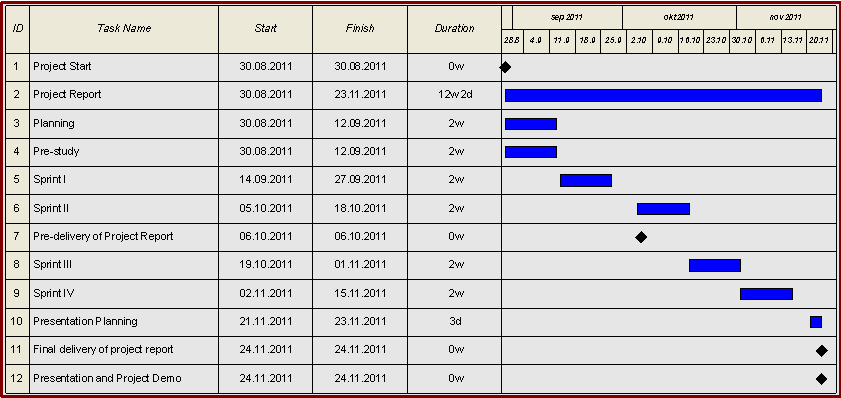
\includegraphics[scale=0.48]{./planning/img/gantt}}
	\caption{Gantt Diagram\label{fig:gantt}}
\end{figure}


%-----------------------------
\section{Project Organization}
%-----------------------------
\label{sec:plan:org}
This section describes how the team was organized, which roles the developers were divided into and the partners of the projet.

\subsection{Project Organization}
%--------------------------------
Our project organization had a flat structure, and the organization chart can be seen in figure \ref{fig:orgchart}. The roles listed in the organization chart are described in table \ref{tab:roles}.

\begin{figure}[htb]
	\noindent\makebox[\textwidth]{%
	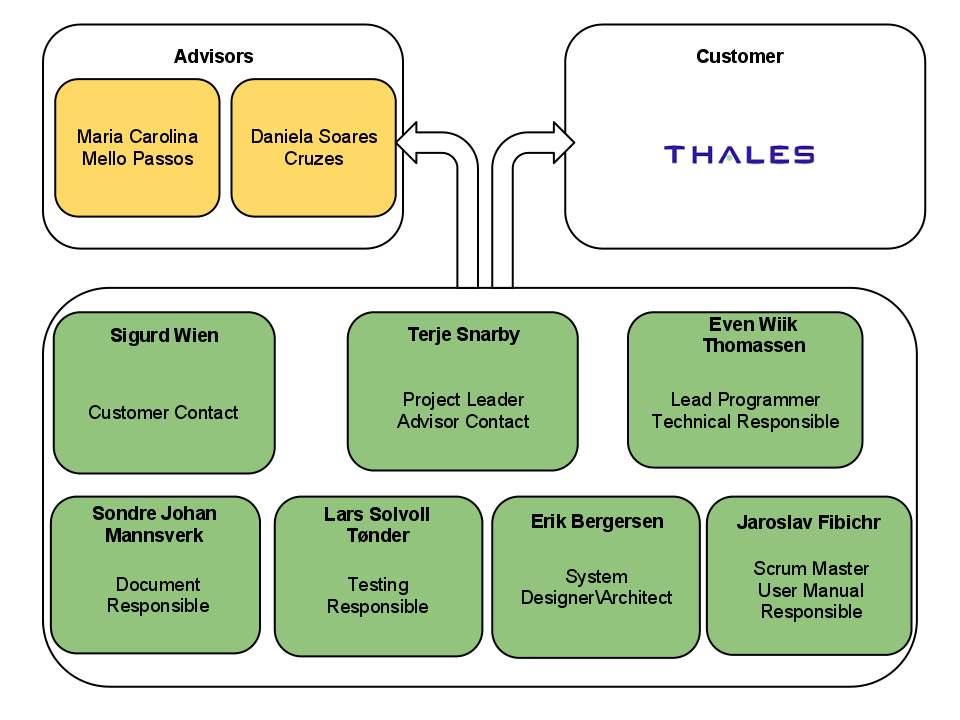
\includegraphics[scale=0.45]{./planning/img/organization}}
	\caption{Project Organization\label{fig:orgchart}}
\end{figure}

\begin{table}[!htb] \footnotesize \center
\caption{Project Roles\label{tab:roles}}
\noindent\makebox[\textwidth]{%
\begin{tabularx}{\textwidth}{l X}
	\toprule
	Role name & Main responsibilities  \\
	\midrule
	Project manager & Responsible for having an overview of the project, delegating tasks and resolving conflicts. \\ 
	Advisor contact & Responsible for distributing information between the team and the advisor. \\
	Organizer & Responsible for setting up and informing the team about the meeting schedule. \\ 
	Document master & Responsible for document quality and quantity. \\ 
	System architect & The lead designer of the system. \\ 
	Lead programmer & Makes sure everyone follows the agreed code standards, and ensures the quality of the code. \\ 
	Customer contact & Responsible for distributing information between the team and the customer. \\ 
	Technically responsible & Finds suitable technical solutions and makes sure that the essential tools are operative. \\ 
	Technology evangelist & Brings in ideas about new technologies and tools. \\ 
	Scrum master & Responsible for \Gls{scrum} meetings. \\ 
	Lead tester & Responsible for test coverage, both unit and end to end, and to ensure the quality of those tests. \\ 
	Secretary & Takes note from each meetings and stores it in the cloud. Responsible for preparing minutes for advisor/customer. \\
	\bottomrule
\end{tabularx}}
\end{table}

\subsection{Partners}
%--------------------
This subsection lists the partners of this project. The customer of this
project is Thales Norway AS, which is located at Lerkendal Stadium,
Strindveien 1, 7030 Trondheim. The customer contacts are listed in
\autoref{tab:plan:customer}. The development team consist of seven student
from \Gls{ntnu}, and is listed in \autoref{tab:plan:devs}. The team is assigned two
advisors from the Department of Computer and Information Science at \Gls{ntnu},
listed in \autoref{tab:plan:advisors}. 

\begin{table}[!htb] \footnotesize \center
\caption{Customers\label{tab:plan:customer}}
\begin{tabular}{l l l}
	\toprule
	Name & Mobile & E-mail \\ 
	\midrule
	Christian Tellefsen & 959 98 765 & christian.telefsen@thalesgroup.com \\ 
	Stig Bjørlykke & 982 29 806 & stig.bjorlykke@thalesgroup.com \\ 
	\bottomrule
\end{tabular}
\end{table}

\begin{table}[!htb] \footnotesize \center
\caption{Developers\label{tab:plan:devs}}
\begin{tabular}{l l l}
	\toprule
	Name & Mobile & E-mail  \\ 
	\midrule
	Terje Snarby & 915 27 390 & snarby@stud.ntnu.no \\ 
	Even Wiik Thomassen & 991 61 929 & evenwiik@stud.ntnu.no \\ 
	Sondre Johan Mannsverk & 948 15 506 & sondrejo@stud.ntnu.no \\ 
	Erik Bergersen & 917 48 305 & eribe@stud.ntnu.no \\ 
	Lars Solvoll Tønder & 976 00 317 & larssot@stud.ntnu.no \\ 
	Sigrud Wien & 472 54 625 & sigurdw@stud.ntnu.no \\ 
	Jaroslav Fibichr & 451 26 314 & jaroslaf@stud.ntnu.no \\ 
	\bottomrule
\end{tabular}
\end{table}

\begin{table}[!htb] \footnotesize \center
\caption{Advisors\label{tab:plan:advisors}}
\begin{tabular}{l l l}
	\toprule
	Name & Mobile & E-mail \\ 
	\midrule
	Daniela Soares Cruzes & 942 49 891 & dcruzes@idi.ntnu.no \\ 
	Maria Carolina Mello Passos & & mariacm@idi.ntnu.no \\ 
	\bottomrule
\end{tabular}
\end{table}


%--------------------------
\section{Quality Assurance}
%--------------------------
\label{sec:plan:qa}
The following section contains internal processes and routines the team used in the project. This includes procesures for meetings, document templates and standards and internal reports.

\subsection{Routines for Ensuring Quality Internally}
%----------------------------------------------------
We decided to organize in pairs when producing items, where the pair reviews each others work. This would be done in an effort to enhance the quality of the project, as we wouldl be able to find more errors, and 
also get a broader perspective on style and solutions.

We also assigned quality assurance responsibilities for three articles: documents, code and tests. The respective team members tried to have a bird's eye overview in their area to catch further errors.

We agreed to have three weekly meetings to accommodate these routines.
\begin{itemize}
	\item Monday 12-14
	\item Wednesday 12-17
	\item Friday 10-13
\end{itemize}

\subsection{Phase Result Approval}
%---------------------------------
To ensure the quality of the sprint deliverables, it was decided that at least one team member would go through the work of another before it is delivered.

We would also present the results to the customer and advisor. They would then have the opportunity to point out problems and misunderstandings, and suggest solutions. This was a result of the \Gls{scrum} methodology: deliveries and deadlines throughout the project, making the progress very visible to the customer and advisors. We reckoned that we should be able to attain success at the end of the project because of the guidance and feedback received during the process of making the utility and report. If a problem appears, we will try to correct it and then reiterate the quality assurance.

\subsection{Procedures for Customer Meetings}
%--------------------------------------------
All customer meetings were to be scheduled with time, place, agenda specified. All background documents relevant to the meetings should also be supplied. This was to ensure efficient and effective meetings.

All customer meetings should be summarised in a document (minute). This document should include:
\begin{itemize}
	\item Time of meeting
	\item Place
	\item Version
	\item Meeting responsible
	\item Names of the attendees
	\item Decisions
	\item Actions
	\item Clarifications
	\item The above should be in sequence according to time
\end{itemize}

This document was to be written and sent to the customer by 12:00 the day after the meeting. If the customer did not approve the minutes, the minutes would again be corrected and sent 12:00 the following day. The customer contact was responsible for the above tasks.

The customer committed to respond to our interactions within two working days.

\subsection{Procedure for Advisor Meeting}
%-----------------------------------------
The weekly advisor meeting will be at 10:30 every Friday unless otherwise stated.

\subsubsection{Agenda for Meeting}
A meeting with the advisor should be scheduled before 14:00 the day before the meeting, and this schedule should include:
\begin{itemize}
	\item Time
	\item Place
	\item Agenda
	\item Status report
	\item Table of reported working hours
	\item Minutes for the last meeting
	\item Other relevant documents
\end{itemize}

\subsubsection{Minutes from Meeting}
The minutes should be written and sent to the advisor for approval before 12:00 the next work day after the meeting. If the advisor should reject the minutes, they should be corrected and re-sent 12:00 the day following the rejection. The minutes should include:
\begin{itemize}
	\item Time of meeting
	\item Place
	\item Version
	\item Names of the attendees
	\item Decisions
	\item Actions
	\item Clarifications
	\item A rough timeline of the above
\end{itemize}

\subsection{Document Templates and Standards}
%--------------------------------------------
The team has specified procedures for templates and file organization.

\subsubsection{Templates the Team Has Created}
All templates were stored under docs/ on Github. The team had templates for:

\begin{itemize}
	\item Meeting agenda
	\item Status report
	\item Meeting minutes
\end{itemize}

\subsubsection{Standard for Organizing Files}
We use Github and Google Docs to store the files included in this project. The
location of a file is dependent on what type the file is. 

\begin{itemize}
	\item All source code is to be saved in the Github \gls{repository} under
		CSjark/. This ensures that all the team members have the current
		version of the code. The structure for this folder:
		\begin{verbatim}
CSjark/
    csjark/  -- today's source/, for source code
        test/  -- for unit tests
        etc/  -- for configuration files
        header/  -- header files used to test the program
    bin/  -- file for executing our program
    docs/  -- for CSjark-specific documentation
    utils/  -- for cpp.exe and fake header files
		\end{verbatim}
	\item All textual documents that are completed will be put in the
		docs/ folder.
	\item All LaTeX documents are stored in the Github \gls{repository}
		under report/. The structure for this folder:
		\begin{verbatim}
report/
    planning/  --   Planning & Requirements section
        img/  --  Images for this section
    sprints/  --  Sprint sections
        img/  --  Images for this section
    evaluation/  --  Evaluation section
    appendices/  --   Appendices section
		\end{verbatim}
	\item Examples of \gls{header}-files and \Gls{lua}-\glspl{script}, \gls{packet} capture-files and information from customer is stored under \Gls{wireshark}/.
	\item All documents or python code should compile before it is pushed to the repository
\end{itemize}

\subsubsection{File Name Standard}
The file name should consist of the name of the document (meeting minutes,
agenda, phasedoc, e.g.) and the date, if applicable.

\subsubsection{Coding Style Standard}
The programming language used to implement the utility specified by the
customer requirements was \Gls{python}. The coding style the team agreed upon was
the \Gls{python} Standard Styling Guide as defined by
PEP8\footnote{Style Guide for Python Code: \url{http://www.python.org/dev/peps/pep-0008/}}.
In addition it was decided that the design should attempt to be pythonic, as detailed by
PEP20\footnote{The Zen of Python \url{http://www.python.org/dev/peps/pep-0020/}}.

\subsection{Version Control Procedures}
%--------------------------------------
The team decided that every relevant digital item should be pushed to our \gls{repository} at github, and be checked out by other participants. Those who worked on a given item were supposed to commit and push their changes often, so that others ccould be as up to date as possible. All digital items were to be labeled with a version number, starting at version one. If an item went under review and was deemed insufficient by the customer, the version number was to also be incremented by one for each revision of the document

Relevant digital items includes source code, documents, picture files, binary blobs, etc.

NB: Google docs was not to be used for version control, so every document written there was also to be pushed to git hub.

\subsection{Internal Reports}
%----------------------------
Some of the internal activities in the team should be documented. This includes:
\begin{itemize}
	\item Activities, what is done, and what remains
	\item Minutes for internal meetings
	\item Milestones, complete/incomplete
	\item Effort registration shall be done daily by each team member.
	\item Sprint backlog should be updated daily by each team member.
\end{itemize}
These documents should follow the templates specified in Templates and Standards (A4) if applicable.


%------------------------
\section{Risk Management}
%------------------------
\label{sec:plan:risk}
The following section lists the possible risk scenarios that could occur in the project, and how they were to be handled. \autoref{tab:risk} shows how to handle the possible risks in the team. Each risk has a consequence and a probability:  \Gls{h}, \Gls{m} or \Gls{l}.
Strategy and actions describes what we were supposed to do to reduce the consequences of the risk, or prevent the risk from happening altogether. Deadline states when we needed to handle the risk.
\begin{description}
\item[R1. Choosing an incompatible technical solution]  The team decides to use a technical solution that is not suited for the given problem, or decides on an implementation that is too time consuming.
\item[R2. Too much focus on report]  We spend too much time working on the report and neglect the implementation. 
\item[R3. Too much focus on implementation]  We spend too much time working on the implementation and neglect writing all the needed documentation for the report.
\item[R4. Illness/Absence]  Members of the team become ill or are otherwise unavailable. 
\item[R5. Key member is absent] A member that has an important responsibility becomes ill.
\item[R6. Conflicts within team]  Internal conflicts which hinders the team's ability to work together. 
\item[R7. Lack of technical competence]  The team lack the needed technical ability to solve the given problem. 
\item[R8. Miscommunication within team]  Team members don’t know what to do, or misunderstands the task given to them. 
\item[R9. Miscommunication with customer]  The team misunderstands the requirements given by the customer. 
\item[R10. Lack of experience with \Gls{scrum}]  The team does not have any experience in doing \Gls{scrum} projects.
\item[R11. Requirements added or modified late in the project] The customer asks us to implement a new, and possibly time consuming requirement, or modifies a requirement in such a way that it needs to be reimplemented, late in the project.
\end{description}

\begin{longtable}{>{\footnotesize}p{0.25\textwidth} >{\footnotesize}p{0.75\textwidth}}
	\caption{Handling Risks}
	\endhead
	\toprule
	Risk ID & R1 \\
	Risk factor & Choosing an incompatible technical solution \\
	Consequences & \Gls{h}: The project will not be completed on time, or at all. \\
	Probability & \Gls{m} \\ 
	Strategy \& actions & Do a good pre-study, consult the customer’s technical expert. \\
	Deadline & During the first sprint.\\
	Responsible & Even and Erik \\
	\midrule
	Risk ID & R2 \\
	Risk factor & Too much focus on report \\
	Consequences & \Gls{m}: The product will not be of a satisfying quality. \\
	Probability & \Gls{m} \\ 
	Strategy \& actions & Plan enough hours to use on the customer product.\\
	Deadline & Continuous\\
	Responsible & Sondre \\
	\midrule
	Risk ID & R3 \\
	Risk factor & Too much focus on implementation \\
	Consequences & \Gls{h}: The documentation will not be good enough, leads to a bad grade. \\
	Probability & \Gls{m} \\ 
	Strategy \& actions & Plan enough hours to use on the report. Write documentation in parallel with implementation when it is possible. Write good requirements that limit the scope of the project. \\
	Deadline & Continuous \\
	Responsible & All \\
	\midrule
	Risk ID & R4 \\
	Risk factor & Illness/Absence \\
	Consequences & \Gls{l}/\Gls{m}/\Gls{h}: Consequences depend on how many members are absent, and how often they are absent. Absence may hinder the progress of the project in different ways.  \\
	Probability & \Gls{m} \\ 
	Strategy \& actions & Make sure several people are proficient in the technical parts of the project. Have backups for the most important roles. \\
	Deadline & Continuous \\
	Responsible & Terje \\
	\midrule
	Risk ID & R5 \\
	Risk factor & Key member is absent \\
	Consequences & \Gls{h} Absence of a key member may greatly hinder the team's process during the period of the absence. \\
	Probability & \Gls{l} \\ 
	Strategy \& actions & The team should be updated on the work of key members, so that a team member they can step in for the key member on important tasks. \\
	Deadline & Continuous \\
	Responsible & All \\
	\midrule
	Risk ID & R6 \\
	Risk factor & Conflicts within team \\
	Consequences & \Gls{m}: May lead to bad morale, which could affect the work of the team. Could also be a waste of time. \\
	Probability & \Gls{m} \\ 
	Strategy \& actions & Not all conflicts are bad. If the conflict is simply a disagreement over technical issues, or the planning of the project, it could benefit the team. All such conflicts should lead to a constructive discussion that the entire team should take part in. Other types of conflicts, that can not positively influence the project should be avoided if possible. The team should agree on specific ground rules. \\
	Deadline & Continuous \\
	Responsible & Terje \\
	\midrule
	Risk ID & R7 \\
	Risk factor & Lack of technical competence \\
	Consequences & \Gls{h}: The team is unable to solve the problem  \\
	Probability & \Gls{h} \\ 
	Strategy \& actions & Make sure the team is proficient in the programming languages and tools that are to be used. Decide on technical solutions that the team is already familiar with. Do a good pre-study of the parts the team is unfamiliar with. Consult with the customer’s technical expert. \\
	Deadline & Continuous \\
	Responsible & All \\
	\midrule
	Risk ID & R8 \\
	Risk factor & Miscommunication within team \\
	Consequences & \Gls{m}: Team members waste time doing nothing, or doing something that is irrelevant. \\
	Probability & \Gls{m} \\ 
	Strategy \& actions & Make sure that everyone knows what to do at all times. Ask questions if you are unsure about your specific task. \\
	Deadline & Continuous \\
	Responsible & Terje \\
	\midrule
	Risk ID & R9 \\
	Risk factor & Miscommunication with customer \\
	Consequences & \Gls{h}: The team waste time on functionality the customer did not want. The delivered product does not do what the customer asked for. \\
	Probability & \Gls{m} \\ 
	Strategy \& actions & Make sure we and the customer have a common understanding of the requirements. Have frequent meetings with the customer, with a weekly demo of new features.  \\
	Deadline & Continuous \\
	Responsible & Sigurd \\
	\midrule
	Risk ID & R10 \\
	Risk factor & Lack of experience with \Gls{scrum} \\
	Consequences & \Gls{m}: The team does not provide the correct documents for the report, which could lead to a bad grade. \\
	Probability & \Gls{m} \\ 
	Strategy \& actions & Learn how to properly do \Gls{scrum}. Have \Gls{scrum} meetings as often as possible. Get feedback on documents from advisor. \\
	Deadline & Continuous \\
	Responsible & Jaroslav \\
	\midrule
	Risk ID & R11 \\
	Risk factor & Important requirements added or modified by customer late in the project \\
	Consequences & \Gls{m}: The team may spend time on implementation when we instead should be finishing up the report, or prepare for the presentation. \\
	Probability & \Gls{h} \\ 
	Strategy \& actions &  Have a good dialog with the customer, and be prepared to say no to new requirements if we do not have the time to complete them.\\
	Deadline & Continuous \\
	Responsible & Jaroslav \\
	\bottomrule
	\label{tab:risk}
\end{longtable}

%=============================
\chapter{Preliminary Study}
%============================
This chapter presents the preliminary study for this project.
In \autoref{sec:pre:similar} we have examined existing solutions, and in
\autoref{sec:pre:method} we provide a description of two popular software
development methodologies.

\Gls{wireshark}, which our \gls{utility} should create \glspl{dissector} for, are described in
\autoref{sec:pre:wireshark}.
\hyperref[sec:pre:langs]{Section \ref*{sec:pre:langs}} contains the different
programming languages we might use, while \autoref{sec:pre:parser}
describes possible solutions for parsing \Gls{c} \gls{header} files.
\hyperref[sec:pre:config]{Section \ref*{sec:pre:config}} outlines possible
configuration libraries, and \autoref{sec:pre:testing} discusses possible unit
testing frameworks. In \autoref{sec:pre:docs} we describe tools for creating
user documentation and \autoref{sec:pre:ide} describes three integrated
development environments.

\hyperref[sec:pre:eval]{Section \ref*{sec:pre:eval}} provides the
justifications for the choices we have made, and in
\autoref{sec:pre:framework} we describe the framework our \gls{utility} will require.
At the end of the chapter, in \autoref{sec:pre:license}, we describe the
license of our \gls{utility}.


%--------------------------
\section{Similar Solutions}
%--------------------------
\label{sec:pre:similar}
We started by searching for existing solutions in the problem space. This
search turned up idl2wrs\footnote{\url{http://wiki.wireshark.org/idl2wrs}}.
The other solution was suggested by our customer,
Asn2wrs\footnote{\url{http://wiki.wireshark.org/Asn2wrs}}.
Both of these solutions are bundled with \Gls{wireshark}.

\subsection{idl2wrs}
%-------------------
A tool for generating \Gls{wireshark} \glspl{dissector} from \gls{idl} files. The tool is written
in \Gls{python}, and generates \glspl{dissector} in \Gls{c} from \gls{idl} specifications. \gls{idl}
 is used as an interface to enable communication between software of different languages, in a 
language-neutral way. It is used for example in \gls{Sun RPC} and \gls{acorba}. 
Since idl2wrs takes input in a different language than our \gls{utility} will, and creates \glspl{dissector}
in a different language than our \gls{utility}, we can not reuse any of its code. Instead we will look
at its architecture and data structures, especially how it generates \glspl{dissector}.

\subsection{Asn2wrs}
%-------------------
Is a tool for generating \Gls{wireshark} \glspl{dissector} from \gls{asnone} \glspl{protocol}. Asn2wrs requires
four input files: an \gls{asnone} \gls{protocol} description, a configuration file and two
template files. Advantages of using Asn2wrs are faster development because of
easier recompilation, and plugins that are easy to distribute. The disadvantage
is that code and \glspl{makefile} are more complex.\cite{asn2wrs} 

Our customer cannot use this solution as it would require them to rewrite 
their \Gls{c} \glspl{struct} to \gls{asnone} descriptions, which would take a 
very long time. But the team can use the asn2wrs code as an example of how to 
create dissectors for \Gls{wireshark}.

%-----------------------------------------
\section{Software Development Methodology}
%-----------------------------------------
\label{sec:pre:method}
In this section we describe two popular software development methodologies,
while \autoref{sec:pre:devchoice} discusses which one we decided to use, and
why.

\subsection{Waterfall}
%---------------------
\label{sec:pre:waterfall}
Waterfall is a software development methodology based on sequential phases.
It consist of the following phases: requirement specification, design,
implementation, integration, testing, deployment, and maintenance. In its pure
form, these phases are non-overlapping and one way only, which means that each
phase must be fully completed before the next can begin. Following the phases are listed in sequentially order.  

\paragraph{Requirement Specification}
Receiving requirements from a customer and then formalising
these into concrete functional and non-functional requirements. These will
again be further broken down into smaller work items that are easy to quantify
in terms of time of use and importance. These metrics may help distinguish
which features are to be prioritised.

\paragraph{Design}
The design is about planning how to implement the features from the
requirement specification. The goal is to make a precise software architecture for the
project that dictates most of the implementation phase. This may include (but
not limited to) making class diagrams, data flow diagrams, state machines, user
interface mock-ups, etc.

\paragraph{Implementation}
Implementing and coding the design made in the design phase on
a component level.

\paragraph{Integration}
Integrating the different components that results from the
implementation phase.

\paragraph{Testing}
Thoroughly test the result of the implementation and
integration. The goal is to find and fix bugs introduced in these
phases.

\paragraph{Deployment}
Delivering the resulting software to the customer. This may include installing the software on their systems. This is also the phase where the customer either accepts or rejects the resulting software.

\paragraph{Maintenance}
Large software projects are almost impossible to make completely bug free, and
therefore a certain amount of maintenance may be required. The obvious tasks
are to either fix or provide viable workarounds for problems that appear during
normal use. Maintenance may also include developing new features that the
customer finds the need for.

\subsection{\Gls{scrum}}
%-----------------
\label{sec:pre:scrum}
\Gls{scrum} is an agile development methodology based on the philosophy that it is
impossible to completely and accurately plan everything in a software project
before you begin. It is therefore more or less based on iterations of the
waterfall phases described in \autoref{sec:pre:waterfall}, but instead of
having these phases being strictly sequential, they are run in a more
'as needed' basis. Each iteration in \Gls{scrum} is called a sprint and typically
lasts between two and four weeks. This time period is fixed for each
project, so the sprint will always end on time. To make this possible, features
that are not completed on time is deferred to a later sprint. Each sprint
should result in a runnable product that potentially could deliver some value
to the customer, even if this requires some redundant work.

\subsubsection{Main \Gls{scrum} Roles}
\begin{description}
	\item[\Gls{scrum} Master] has the responsibility of maintaining the process and
		for removing obstacles for other team members. In short, the \Gls{scrum}
		master tries to keep the other team members focused on their tasks.
	\item[Product Owner] represents and speaks for the customer. Not
		necessarily a part of the customer's organization, but must have the
		stated authorities.
	\item[Team Members] are responsible for creating and delivering the product.
		Should consist of a self organizing team of five to nine persons with
		a cross functional skill set.
\end{description}

\subsubsection{\Gls{scrum} Artifacts}
\begin{description}
	\item[Product Backlog] contains a high level description of all the desired
		features for the project. These should be prioritised based on their
		business value and evolve along with the project.
	\item[Sprint Backlog] contains what the team is committed to complete over
		the next sprint. These commitments are features broken down into work
		items. These items should not be larger than 16 hours of work, and they
		should be described so that everyone in the team could contribute to
		implementing them.
	\item[Burn Down Chart] A daily updated chart consisting of what work
		remains in the sprint. Its purpose is both to show what work to do next
		and to give a visual representation of the work progress.
\end{description}

A sprint begins with the sprint planning meeting, which consists of two stages. In the first, the team and the product owner prioritizes the product backlog. In the second, the team discusses what features they can commit to, based on priority, and break these down into work items, which are added to the sprint backlog. This should include giving each item an estimated completion time.

The sprint itself consists of producing what is required for completing work
items, updating the burn down chart, and daily \Gls{scrum} meetings. In these daily
meetings each team member provides a short update of what they did the day
before, what they plan to do today and what problems might be in their way.
These problems should not be discussed in this meeting, but rather dealt with
separately after the meeting, which is the \Gls{scrum} master's responsibility.

At the end of the sprint cycle, the team should hold a \Gls{scrum} review meeting.
In this meeting the team should discuss what was completed and what was not, and
demonstrate the completed features for the customer.	

After the review meeting, a separate retrospect meeting should be held with all
the team members, where all members share their reflections of how the sprint
went and on how we could improve for the next sprint. This is important for improving the
process.


%------------------
\section{\Gls{wireshark}}
%------------------
\label{sec:pre:wireshark}
\begin{wrapfigure}{r}{3.5cm}
	\vspace{-10pt}
	
\includegraphics[width=3.5cm]{./planning/img/wireshark_logo}
	\vspace{-20pt}
\end{wrapfigure}
\Gls{wireshark}\footnote{\url{http://www.wireshark.org/}} is a free, open source
network \gls{protocol} analyzer. It lets you capture and browse traffic running
through a computer network. \Gls{wireshark} is currently being developed by the
\Gls{wireshark} team, a group of networking experts spanning the globe.\cite{WiresharkORG} Because of
its rich set of features and ease of use, \Gls{wireshark} is the de facto standard in
many different industries and the educational community. \Gls{wireshark} is able to
dissect and display data from a plethora of different \glspl{protocol}. One of its
strengths lies in the ease of which developers can add their own \glspl{dissector},
\gls{post-dissector} and taps.

\Glspl{dissector} can be written in either \Gls{c} or \Gls{lua}. Most \glspl{dissector} are written in \Gls{c}
for increased speed. \Gls{lua}-scripts are mostly used as prototypes or to process
non time crucial data as they don't need compilation to be used. Our customer
uses \Gls{wireshark} not only to browse through and filter regular networking
traffic, but also for monitoring \gls{ipc} where it is
important to have a tool which can easily be extended to dissect and display
structures and data types unique to the organization.

Our \gls{utility} should read \Gls{c} \gls{header} files and create \Gls{wireshark} \glspl{dissector} written
in \Gls{lua} for \glspl{struct} found in the \gls{header} files.


%------------------------------
\section{Programming Languages}
%------------------------------
\label{sec:pre:langs}
The \glspl{dissector} we have to generate are written in \Gls{lua}, and we have looked at
both \Gls{java} and \Gls{python} programming language for our \gls{utility}. In this section we
describe these different languages. In \autoref{sec:pre:langchoice} we describe
which language we selected and why.

\subsection{\Gls{lua}}
%---------------
\begin{wrapfigure}{r}{2.5cm}
	\vspace{-10pt}
	
\includegraphics[width=2.5cm]{./planning/img/lua_logo}
	\vspace{-20pt}
\end{wrapfigure}
\Gls{lua}\footnote{\url{http://www.lua.org/}} is a multi-paradigm, dynamically typed
programming language which is designed to be lightweight so it can easily be
embedded into applications. \Gls{lua} has only a few basic data structures: boolean,
numbers, strings and table. Still \Gls{lua} implements advanced features such as
first-class functions, garbage collection, closures, coroutines and dynamic
module loading. \Gls{lua} was created in 1993 at the Pontifical Catholic University
of Rio de Janeiro, in Brazil.\cite{LuaORG}

The output of our \gls{utility} will be \Gls{wireshark} \glspl{dissector} written in \Gls{lua}. While
\Gls{wireshark} supports \glspl{dissector} written in both \Gls{c} and \Gls{lua}, \Gls{lua} is preferred
because they can be added without recompiling \Gls{wireshark}. This is important since some of Thales customers do not allow recompiled versions of Wireshark. \Gls{lua} \glspl{dissector}
interface with \Gls{wireshark} through a simple \Gls{api}.

\subsection{\Gls{java}}
%----------------
\label{sec:pre:java}
\begin{wrapfigure}{r}{1.3cm}
	\vspace{-30pt}
	
\includegraphics[width=1.3cm]{./planning/img/java_logo}
	\vspace{-30pt}
\end{wrapfigure}
\Gls{java}\footnote{\url{http://java.com/}} is an object-oriented, structured,
imperative, statically typed programming language. It was originally developed
by Sun Microsystems, which is now a subsidiary of Oracle Corporation. \Gls{java} was
released in 1995, and it derived much of its syntax from \Gls{c} and \Gls{c++}, but with
fewer low-level facilities. \Gls{java}’s strength are portability, automatic memory
management, security, good documentation and an extensive standard \gls{library}.\cite{JavaCOM}
\Gls{java} has several tools and \glspl{library} of varying quality for creating \glspl{parser},
for example \gls{antlr} and \gls{javacc}. A detailed description of \gls{antlr} can be found in 
\autoref{sec:pre:antlr}.

\subsection{python}
%------------------
\label{sec:pre:python}
\begin{wrapfigure}{r}{2cm}
	\vspace{-20pt}
	
\includegraphics[width=2cm]{./planning/img/python_logo}
	\vspace{-20pt}
\end{wrapfigure}
\Gls{python}\footnote{\url{http://www.python.org/}} is a general-purpose,
multi-paradigm, object-oriented, imperative, dynamically typed programming
language. It was created by Guido van Rossum, and is today developed by \Gls{python}
Software Foundation and the \Gls{python} community. \Gls{python}’s strength include
automatic memory management, large and comprehensive standard \gls{library},
portability, powerful but very clear, concise and simple syntax.\cite{PythonORG} There exists
several pure \Gls{python} \glspl{library} for creating \glspl{lexer} and \glspl{parser}, like \gls{aply},
\gls{pycparser} and cppheaderparser. These are described further in
\autoref{sec:pre:parser}.


%-----------------------------------
\section{Parsers Libraries \& Tools}
%-----------------------------------
\label{sec:pre:parser}
This section contains various tools and \glspl{library} we have looked at for solving
the challenge of parsing \Gls{c} \gls{header} files. They range from language-independent
tools like \gls{agcc} and \Gls{clang} to \Gls{python}-only \glspl{library} like \Gls{aply} and \gls{pycparser}. The
justification for the \glspl{library} we selected can be found in
\autoref{sec:pre:parserchoice}.

\subsection{\gls{antlr}}
%-----------------
\label{sec:pre:antlr}
\begin{wrapfigure}{r}{2.5cm}
	\vspace{-20pt}
	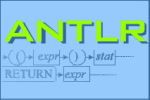
\includegraphics[width=2.5cm]{./planning/img/antlr_logo}
	\vspace{-20pt}
\end{wrapfigure}
\gls{antlr}\footnote{\url{http://www.antlr.org/}}, ANother Tool for Language
Recognition, is a compiler toolkit for creating \glspl{lexer} and \glspl{parser} from grammar
files. It can create these compilers for several different target languages,
including \Gls{java} and \Gls{python}. There exists \gls{antlr} grammar files for the challenges
we are facing: parsing \Gls{c}, \Gls{c} \gls{preprocessor} step and parsing \gls{asnone}. These grammars
configure \gls{antlr} to create \Gls{java} \glspl{lexer} and \glspl{parser} which reads and validates
inputted source code files.

\subsection{PLY}
%---------------
\Gls{aply}\footnote{\url{http://www.dabeaz.com/ply/}} is a \Gls{python} alternative to the
popular \gls{lexer} and \gls{parser} compilers lex and yacc. It also comes with a 95\%
completed \Gls{c} \gls{preprocessor} in case we are required to modify the \gls{preprocessor}
for our \gls{utility}. Other special purpose \glspl{parser} like \gls{pycparser} and
cppheaderparser depends on \Gls{aply}. These are described later in this section.

\subsection{\gls{pycparser}}
%---------------------
\label{sec:pre:pycparser}
There are two \Gls{python} \glspl{library} for parsing \Gls{c} with the same name, but different
capitalization, \gls{pycparser}\footnote{\url{http://code.google.com/p/pycparser/}}
and PyCParser\footnote{\url{https://github.com/albertz/PyCParser}}. While they
both aim to solve almost the same problem, the first one appears to have better
documentation, is a more mature project and support more of the \Gls{C99}
specification. \gls{pycparser} requires \Gls{aply} to work.

\subsection{cppheaderparser}
%---------------------------
Cppheaderparser\footnote{\url{http://sourceforge.net/projects/cppheaderparser/}}
is a \gls{parser} for \Gls{c++} \gls{header} files written in \Gls{python}. It is an alternative for
\gls{pycparser} in case we need to parse \Gls{c++} files instead of simple \Gls{c} \gls{header} files.
It also depends on \Gls{aply}.

\subsection{GCC}
%---------------
\label{sec:pre:gcc}
\begin{wrapfigure}{r}{1.5cm}
	\vspace{-20pt}
	
\includegraphics[width=1.5cm]{./planning/img/gcc_logo}
	\vspace{-20pt}
\end{wrapfigure}
GNU Compiler Collection\footnote{\url{http://gcc.gnu.org/}} (\Gls{agcc}) is a
compiler system which has front ends which parse \Gls{c} and \Gls{c++} code, and is written
in \Gls{c} and \Gls{c++}. It can be used in our \gls{utility} as an external tool which does the
parsing and then outputs an intermediate language representation which we can
parse/search to find the \Gls{c} \gls{struct} definitions. Its drawbacks are a lack of
flexibility if we need to change its behaviour, and we will still need to write
a custom \gls{parser} or use something like \gls{GCC-XML} and an \gls{axml} \gls{parser}.

\subsection{\Gls{clang}}
%-----------------
\label{sec:pre:clang}
\begin{wrapfigure}{r}{2.5cm}
	\vspace{-20pt}
	
\includegraphics[width=2.5cm]{./planning/img/llvm_logo}
	\vspace{-20pt}
\end{wrapfigure}
\Gls{clang}\footnote{\url{http://clang.llvm.org/}} is a compiler front end for \Gls{c}, 
\Gls{c++}, \Gls{Objective-C} and \Gls{Objective-C++}, written in \Gls{c++}. \Gls{clang} differ from \Gls{agcc} as it
behaves as a \gls{library} rather than an external tool, but for \Gls{java} we will have to
use it like \Gls{agcc} because there are no \Gls{java}-\Gls{clang} bindings. It supports
outputting the \gls{AST} as \Gls{axml}, which our \gls{utility} then will need to
parse. \Gls{clang} provides bindings for \Gls{python} so there it can be used as a \gls{library},
but its main drawback is, like \Gls{agcc}, a lack of flexibility. \Gls{clang} is a part of
the LLVM toolkit.


%---------------------------------
\section{Configuration Frameworks}
%---------------------------------
\label{sec:pre:config}
This section looks at different configuration frameworks for \Gls{python}. Which we
selected and why is explained in \autoref{sec:pre:configchoice}.

Our \gls{utility} needs a flexible configuration, as some of the information we
shall display does not exist in the files we parse. For example there are no
clear relationship between enumerated values in messages and their names.
These must be provided through a configuration.

\subsection{\gls{asnone}}
%-----------------
\gls{asn1} (\gls{asnone}) for describing data
structures, the standard is defined by \Gls{iso} 8824. \gls{asnone} is used for
representing, encoding, transferring and decoding of data. It provides a
fundamental tool to be used in application, which make it possible to exchange
information in a independent way. There exist two \Gls{python} \glspl{library} for parsing
of  \gls{asnone}, but neither support the 3.x \gls{branch} of \Gls{python}, which we require.

\subsection{\Gls{yaml}}
%----------------
\label{sec:pre:yaml}
\begin{wrapfigure}{r}{3cm}
	\vspace{-30pt}
	
\includegraphics[width=3cm]{./planning/img/pyyaml_logo}
	\vspace{-30pt}
\end{wrapfigure}
\Gls{yaml}\footnote{\url{http://yaml.org/}} (\Gls{yaml} Ain't Markup Language) is a \gls{data serialization} format.
It is designed to be easy to read and write for humans.
\Gls{yaml} syntax was designed to be easily mapped to data types common to most
high-level languages. While most programming languages can use \Gls{yaml} for data
serialization, \Gls{yaml} excels in working with those languages that are
fundamentally built around the three basic primitives. These include the new
wave of agile languages such as \Gls{perl}, \Gls{python}, \GLS{php}, \Gls{Ruby}, and \Gls{Javascript}.

PyYAML\footnote{\url{http://pyyaml.org/}} is a \Gls{yaml} \gls{parser} for the \Gls{python}
programming language, and it is available for both the 2.x and 3.x \gls{branch} of
\Gls{python}. It is licensed under the \Gls{mit} license.

\subsection{configparser}
%------------------------
configparser\footnote{\url{http://docs.python.org/py3k/\gls{library}/configparser.html}}
is a \Gls{python} module to manage user-editable configuration files. The
files are organized into sections, and each section can contain name-value
pairs for configuration data. Value interpolation using \Gls{python} formatting
strings is also supported, to build values that depend on one another.

configparser module is a part of \Gls{python} standard \gls{library}, and therefore does
not require installation or configuration to use.

\subsection{ConfigObj}
%---------------------
ConfigObj\footnote{\url{http://www.voidspace.org.uk/python/configobj.html}} is
a simple but powerful config file reader and writer (originally based on
ConfigParser). Its main feature is that it is very easy to use, with a
straightforward programmer's interface and a simple syntax for config files.
Among others, it has these additional features:
\begin{itemize}
	\item Nested sections (subsections), to any level
	\item List values
	\item Multiple line values
	\item String interpolation (substitution)
	\item Integrated with a powerful validation system
\end{itemize}

\noindent Currently, ConfigObj module exists only for \Gls{python} up to version
2.7. It is under \Gls{bsd} license.


%--------------------------------
\section{Unit Testing Frameworks}
%--------------------------------
\label{sec:pre:testing}
There are many different unit testing frameworks for \Gls{python}. We have evaluated
three of them, to see which best suits our \gls{utility}, which we describe in this
section. In \autoref{sec:pre:testchoice} we describe which we selected and why.

\subsection{py.test}
%-------------------
py.test\footnote{\url{http://pytest.org/latest/}} is a mature, full-featured testing
tool. It runs on \Gls{python} 2.4-3.2, PyPy and Jython-2.5.1 intepreters on both
Windows and Posix platforms. It is well documented and popular in the \Gls{python}
community. The best known project which uses it is PyPy, which has over 16,000
unit tests. py.test discoverers tests automatically by searching for modules,
classes, functions and methods which starts with "test\_". It uses the assert
statement to test variables and values. These implicit behaviours make tests
easier and faster to write, but harder to learn and understand.

\subsection{nose}
%----------------
nose\footnote{\url{http://readthedocs.org/docs/nose/en/latest/}} testing
framework extends \Gls{python}'s unittest \gls{library} to make testing easier.
It provides an alternative test discovery and running process for unittest,
which is intended to mimic the behavior of py.test as much as reasonably
possible without resorting to too much magic. nose support easy-to-write
plugins, and it comes bundled with the most popular ones. It supports both
\Gls{python} 2.x and 3.x \glspl{branch}.

\subsection{Attest}
%------------------
\label{sec:pre:attest}
\begin{wrapfigure}{r}{3.2cm}
	\vspace{-20pt}
	
\includegraphics[width=3.2cm]{./planning/img/pocoo_logo}
	\vspace{-30pt}
\end{wrapfigure}
Attest\footnote{\url{http://packages.python.org/Attest/}} is a test automation
framework for \Gls{python}, emphasising modern idioms and conventions. It supports
test collecting using \Gls{python} decorators, introspection of the assert statement,
treating tests as \Gls{python} modules rather than scripts. Attest is a rather young
framework, with limited features and documentation. Attest is a sub-level
project of the Pocoo project.

\subsection{coverage.py}
%-----------------------
coverage.py\footnote{\url{http://nedbatchelder.com/code/coverage/}} is a tool
for measuring code coverage of \Gls{python} programs. It is typically used to measure
the effectiveness of unit tests, by showing which parts of the code are
exercised by tests. coverage.py support \Gls{python} 2.3 to 3.2. It can output
results in plain text, \Gls{html} and \Gls{axml}.


%---------------------------------
\section{User Documentation Tools}
%---------------------------------
\label{sec:pre:docs}
Some of the non-functional requirements for our \gls{utility} is user documentation.
In this section we describe a tool for writing such documentation, and a free
hosting site for our user documentation.

\subsection{Sphinx}
%------------------
\begin{wrapfigure}{r}{2.7cm}
	\vspace{-20pt}
	
\includegraphics[width=2.7cm]{./planning/img/sphinx_logo}
	\vspace{-20pt}
\end{wrapfigure}
Sphinx\footnote{\url{http://sphinx.pocoo.org/}} is a \Gls{python} tool for writing
documentation, that makes it easy to create intelligent and beautiful
documentation. It is used for the standard \Gls{python} documentation, and it is
popular in the \Gls{python} community. Sphinx uses reStructuredText as its markup
language, which is a easy-to-read, what-you-see-is-what-you-get plain text
markup syntax and \gls{parser} system. Our use case for sphinx is writing
documentation for our \gls{utility}, how to use it and configure it. Sphinx can
generate output in several different formats, including \Gls{html} and latex/pdf.

\subsection{Read the Docs}
%-------------------------
\begin{wrapfigure}{r}{1.2cm}
	\vspace{-20pt}
	
\includegraphics[width=1.2cm]{./planning/img/readthedocs_logo}
	\vspace{-20pt}
\end{wrapfigure}
Read the Docs\footnote{\url{http://readthedocs.org/docs/read-the-docs/}} is a
free hosting of documentation for the open source community. It supports Sphinx
docs written with reStructuredText, and it can automatically pull from Git,
Subversion, Bazaar, and Mercurial repositories. We can configure it so it
automatically pulls and compiles our user documentation from our github
repository whenever we push any changes.


%-------------------------------------------
\section{Integrated Development Environment}
%-------------------------------------------
\label{sec:pre:ide}

\subsection{PyCharm}
%-------------------
\begin{wrapfigure}{r}{3.5cm}
	\vspace{-20pt}
	
\includegraphics[width=3.5cm]{./planning/img/pycharm_logo}
	\vspace{-20pt}
\end{wrapfigure}
PyCharm\footnote{\url{http://www.jetbrains.com/pycharm/}}
is a cross platform, proprietary \Gls{ide} for \Gls{python}. It has good support
for text editing, syntax highlighting, auto indentation, code navigation, code
completion and automatic error checking. There is also a decent debugger and
unit test support that can help finding errors and integrated version control
support (including git), which makes it easy to synchronize with a remote
repository. Most mentioned functions is also paired with keyboard shortcuts.

The downside with PyCharm is that it requires a relative expensive license. It
is, however, possible to apply for classroom licenses that are free of charge.
The latter is a requirement to make this \Gls{ide} a viable option.

\subsection{PyScripter}
%----------------------
\begin{wrapfigure}{r}{3cm}
	\vspace{-20pt}
	
\includegraphics[width=3cm]{./planning/img/pyscripter_logo}
	\vspace{-20pt}
\end{wrapfigure}
PyScripter\footnote{\url{http://code.google.com/p/pyscripter/}}
is a Windows only, open source \Gls{ide} for \Gls{python}. It has support for
basic text editing functions relevant to programming like syntax highlighting,
auto indentation, code completion, debugger and file management. It also has
some support for navigating the code, for example by offering to find the next
point in the code that references a certain variable or function. The mentioned
function mostly has keyboard shortcuts.

It does not have support for automatic error checking in the program, so it
will not alert the user of spelling and syntax errors. It also lacks integration
with any version control systems like git or svn. The code completion and
code navigation is a little lacking. It will for example not suggest importing
files if you reference a class from another module and it cannot give a
complete list of usages of a function.

\subsection{\gls{vim}}
%---------------
\begin{wrapfigure}{r}{1.5cm}
	\vspace{-20pt}
	
\includegraphics[width=1.5cm]{./planning/img/vim_logo}
	\vspace{-20pt}
\end{wrapfigure}
\gls{vim}\footnote{\url{http://www.vim.org/}} is cross-platform, open source text
editor originally created for the Amiga. It is not regarded as an \Gls{ide}, but it
provides all the regular features of text editors, including syntax
highlighting, auto-completion, auto-indentation, searching, multiple undo and
redo. It can be configured to support almost everything modern \Gls{ide}’s support,
and its extensive customizability is considered parts of its strength. But it
is also parts of its weakness, it is very difficult for new \gls{vim} users to learn
how to use it effectively. Therefore we do not suggest any team member which is
not already experienced with \gls{vim} to try it.

\subsection{Summary}
%-------------------
PyCharm is by far the best \Gls{ide} evaluated in terms of functionality, and it is
the one that mirrors \Gls{Eclipse} the most, which is an advantage, since most team
members are best acquainted with \Gls{Eclipse}. It will be the recommended \Gls{ide} for
this project, given that we can acquire classroom licenses.

On the other hand, there is no real reason to dictate the use of \Gls{ide}, since
what determines the productivity of a team member is more how well you know
the specific tool you are using. It will therefore be up to each team member
to choose what \Gls{ide}/text editor they want to use.


%----------------------------------
\section{Evaluation and Conclusion}
%----------------------------------
\label{sec:pre:eval}
In this section we provide a justification for the choices we have made in
regards to process, programming language, and \glspl{library} we will use. Then
in \autoref{sec:pre:framework} we give a brief description of the framework
we will construct for our \gls{utility}.

\subsection{Development Process Choice}
%--------------------------------------
\label{sec:pre:devchoice}
We have chosen \hyperref[sec:pre:scrum]{\Gls{scrum}} for our development strategy.
We do not have a lot of experience with software development either
individually or as a team, so we have little personal knowledge of how much
we are able to produce, and the task may present challenges that we are not
prepared for when the project starts. For these reasons we believe that we
need to take an agile approach to this project. This way, we may both learn as
we go, and adjust later iterations by the result of the previous. We may also
have something to deliver even if we do not have time to implement all the
desired features.

The \Gls{scrum} methodology fits these goals perfectly, and is therefore a natural
choice. The risk factor here is that all team members are mostly unfamiliar
with \Gls{scrum}, while we have at least a little knowledge of waterfall. We do,
however, think that the time and risk of learning will not outweigh
the benefit it will give us over waterfall.

\subsection{Programming Language Choice}
%---------------------------------------
\label{sec:pre:langchoice}
We originally selected \hyperref[sec:pre:java]{\Gls{java}} as our programming
language because it would run on all the platforms required, it offered
automatic memory management so it would be easier to debug, and it was the only
language everyone on the team had experience with.

We looked at \hyperref[sec:pre:antlr]{\gls{antlr}} for generating a
\Gls{c} \gls{lexer} and \gls{parser} in \Gls{java}, which looked very promising. It also provided
grammar files for creating a \Gls{c} \gls{preprocessor} in \Gls{java}. Closer evaluation revealed
that the \Gls{c} \gls{preprocessor} grammar was written in 2006, and had stopped working in
2008 as newer versions of \gls{antlr} was not backwards compatible. Also the
generated \Gls{c} \gls{parser} only validated \Gls{c} code, it did not create an \gls{AST} which we could traverse.
This meant that using \Gls{java} and \gls{antlr} would
require us to modify these grammars to suite our needs, and \gls{antlr}'s lack of
documentation became a significant risk for our project.

These issues and feedback from our customer made us evaluate \Gls{python} for
developing our \gls{utility}. We found several \glspl{library} for parsing \Gls{c} files, and
even one for parsing \Gls{c++} \gls{header} files. These are described in
\autoref{sec:pre:parser}.

We decided to use \hyperref[sec:pre:python]{\Gls{python}} for this project because
the parsing \glspl{library} for \Gls{python} came in working condition with decent
documentation, and because we were able to create a small working prototype
in \Gls{python} in just a few hours. We estimate that it would take at least a week
to achieve the same result in \Gls{java}.

A challenge with our decision is the fact that not all team members have
sufficient experience with \Gls{python}. Most team members must therefore do some
self study before we start the first sprint.

\subsection{Parsers Libraries \& Tools Choice}
%---------------------------------------------
\label{sec:pre:parserchoice}
We outlined three different approaches for parsing \Gls{c} \gls{header} files. The first approach is to
write a custom \gls{parser} ourself, the second is to use a \Gls{c} parsing \gls{library}, and the
third is to use a toolkit \gls{parser} like \hyperref[sec:pre:gcc]{\Gls{agcc}} and
\hyperref[sec:pre:clang]{\Gls{clang}}.

We felt that writing our own \Gls{c} \gls{parser} with \Gls{c} \gls{preprocessor} would possibly take
up a lot, if not all, of the available project time. The third option would add
a large dependency which our customer want to avoid if possible. \Gls{agcc} and \Gls{clang}
can be challenging to install and use on Windows.

Therefore using a \Gls{c} \gls{parser} \gls{library} would be the best solution, and as mentioned
above, \Gls{java} with \gls{antlr} proved challenging. So we evaluated \Gls{python} \gls{parser}
\glspl{library}.

We decided to use \hyperref[sec:pre:pycparser]{\gls{pycparser}}. We favored \gls{pycparser}
over PyCParser and cppheaderparser because it has better documentation, it
seemed to be a more mature project, and it supports the most of the \Gls{C99}
specification. \gls{pycparser} depends on \Gls{aply}, so our \gls{utility} will also depend on it.

For \Gls{c} \gls{preprocessor} we have selected to use a tool for Windows which comes with
\gls{pycparser}, on Mac we will use the one which comes with XCode, and on other
platforms we will either use \Gls{agcc} or tools which comes with the platform. If we
need to modify a \Gls{c} \gls{preprocessor} we might use \Gls{aply}'s incomplete \Gls{c} \gls{preprocessor}.

\subsection{Configuration Framework Choice}
%------------------------------------------
\label{sec:pre:configchoice}
We have listed a summary of some of the advantages and drawbacks of the
different configuration frameworks we looked at in \autoref{tab:pre:config}.
\begin{table}[htbp] \footnotesize \center
\caption{Configuration summary\label{tab:pre:config}}
\noindent\makebox[\textwidth]{%
\begin{tabularx}{1.1\textwidth}{X X X X X}
	\toprule
	& \Gls{yaml} & configparser & ConfigObj & \gls{asnone} \\
	\midrule
	Advantages &
	+Simplicity\newline +Flexibility &
	+Easy to use &
	+Easy to use\newline +Flexibility\newline +Nesting\newline +Type \newline\hspace*{3mm}validation &
	+Customer \hspace*{3mm}wants it \\
	\addlinespace
	Drawbacks &
	-External \gls{library}\newline -No type \newline\hspace*{2mm}validation &
	-Lacks nesting\newline -Lacks lists\newline -No type \newline\hspace*{2mm}validation &
	-External \gls{library}\newline -Lacks lists &
	-External \gls{library}\newline -Too generic \\
	\addlinespace
	Latest version & 3.10 & 3.2 & 4.7.2 & 0.0.13 \\
	\Gls{python} \gls{branch} & 2.7 and 3.3 & 2.7 and 3.3 & 2.7 & 2.7 \\
	License & \Gls{mit} & PSF L & \Gls{bsd}-new & \Gls{bsd} \\
	\bottomrule
\end{tabularx}}
\end{table}

We decided to use \hyperref[sec:pre:yaml]{YAML} for handling configuration
files, as it covered most of our requirements. Because we decided to use the
latest version of \Gls{python}, version 3.2.2, the range of possible configuration
frameworks was reduced. Therefore, although \gls{asnone} and ConfigObj are very
suitable for our task, they were eliminated (those \glspl{parser} are available
only up to version 2.7), which left us 2 main possibilities: \Gls{yaml} and
configparser. configparser turned out to be insufficient for us, mainly because
it lacked lists. These we need for description of hierarchical structures of
the \Gls{c} \glspl{header}. \Gls{yaml} has only two minor disadvantages we should be aware of.
First, there is no type validation mechanism, so we will have to create our
validation manually. Second, it is an external \gls{library}. We find this drawback
minor for now but it can turn out to be a problem in the future. Except for
these issues, \Gls{yaml}, more specifically pyYAML, seems to have a good potential
for creating flexible configuration support for our \gls{utility}.

\subsection{Unit Testing Framework Choice}
%-----------------------------------------
\label{sec:pre:testchoice}
The three frameworks we looked at  are very similar, being modern \Gls{python}
testing frameworks. They differ in maturity and what is often called magic in
the \Gls{python} community.

py.test is the most mature but also the most magic, it uses a lot of
introspection to discover tests and it has no \Gls{api}. nose is heavily influenced
by py.test, but it tries to be more explicit, and provides an \Gls{api}. Attest is
the youngest testing framework, and like nose, has less magic and focuses on
providing a very pythonic \Gls{api}. Being the youngest also means it has the least
documentation, functionality and plugins. Therefore Attest might be the easiest
testing framework to learn. Therefor we decided to use
\hyperref[sec:pre:attest]{Attest} for unit testing of our \gls{utility}.

\subsection{Our Framework}
%-------------------------
\label{sec:pre:framework}
Our \gls{utility} will need to take as input \Gls{c} \gls{header} files, search through them to
find \gls{struct} definitions, and create \Gls{lua} scripts which dissects the \glspl{struct} in
\hyperref[sec:pre:wireshark]{Wireshark}.

To find the \glspl{struct} we will use \gls{pycparser} to parse the input files, create an
\gls{AST}, and to find the \gls{struct} definitions. We will use pyYAML to
read configuration from file, which together with the \gls{struct} definitions will
be placed in some suitable data structures for generating \glspl{dissector}.

The versions of the different tools and \glspl{library} we are using can be found in
\autoref{tab:pre:versions}.
\begin{table}[!h] \footnotesize \center
\vspace{-10pt}
\caption{Versions of tools and \glspl{library}\label{tab:pre:versions}}
\begin{tabular}{l l l}
	\toprule
	Library/Tool & Version & Why \\
	\midrule
	\Gls{python} & CPython 3.2.2 & Latest stable standard \Gls{python} implementation \\
	\gls{pycparser} & 2.05-dev & Development version, for \_Bool support \\
	pyYAML & 3.10 & Latest stable version \\
	\Gls{aply} & 3.4 & Latest stable version \\
	Attest & 0.6-dev & Development version, for \Gls{python} 3.2 support \\
	Sphinx & 1.0.8 & Latest stable version \\
	WireShark & 1.7.0-SVN & Latest nightly build, for \Gls{lua} support \\
	\bottomrule
\end{tabular}
\vspace{-10pt}
\end{table}


%-----------------------------
\section{IP Rights \& License}
%-----------------------------
\label{sec:pre:license}
The customer has explained that they do not intend to distribute our \gls{utility},
and that we are free to license it as open source if we want to, under
whichever license we feel is most suited. They suggested GNU\footnote{\url{http://www.gnu.org/}} \Gls{gpl} as \Gls{wireshark}
is released under it.

We needed to consider the licenses of the \glspl{library} and tools we depend upon
when we decided which license to use. This is summarized by
\autoref{tab:pre:licenses}.
\begin{table}[!h] \footnotesize \center
\vspace{-20pt}
\caption{Licenses\label{tab:pre:licenses}}
\begin{tabular}{l l}
	\toprule
	\Gls{wireshark} & GNU \Gls{gpl} \\
	\Gls{aply} & \Gls{bsd}-new \\
	\gls{pycparser} & \Gls{bsd}-new \\
	pyYAML & \Gls{mit} \\
	\midrule
	Our \gls{utility} & \Gls{bsd}-new \\
	\bottomrule
\end{tabular}
\vspace{-10pt}
\end{table}

\noindent Some of the requirements for our \gls{utility} might require us to modify
the \Gls{c} \gls{preprocessor} in \Gls{aply} and the \gls{pycparser} \gls{library}, which made us consider
the new 2-clause \Gls{bsd} license the most suited for us. Since it also gives us the
option to later move to a more restrictive license like \Gls{gpl}, we decided to use
it.

%=====================
\chapter{Requirements}
%=====================
\label{chap:req:requirements}
This chapter describes a \gls{utility} that creates \Gls{wireshark} \glspl{dissector} from \Gls{c}
\gls{header} files. The \glspl{dissector} must interpret \gls{binary} representations of \Gls{c}
\glspl{struct}. In \autoref{sec:req:list} we give a high level overview of the
\gls{utility} and lists all the functional and non-function requirements, 
while \autoref{sec:req:usecases} provides use cases for the \gls{utility}, 
and \autoref{sec:prodbacklog} contains the complete product backlog.

%-----------------------------
\section{List of Requirements}
%-----------------------------
\label{sec:req:list}

\subsection{Overview}
%-----------------
We are to create a \gls{utility} that allows \Gls{wireshark} to interpret the \gls{binary}
representations of \Gls{c}-language \glspl{struct}. While \Gls{c} \glspl{struct} seldom are exchanged
across networks, they are sometimes used in \gls{ipc}. The
purpose of the \gls{utility} described here is to provide \Gls{wireshark} with the
capability of automatically dissecting the \gls{binary} representation of a \Gls{c} \gls{struct},
as long as its definition is known.

The expected work flow for the \gls{utility} is to read one or more \Gls{c} \gls{header} files,
which contain \gls{struct} definitions, and output \Gls{wireshark} \glspl{dissector}, implemented
in \Gls{lua} scripts. A configuration file or source code annotations in the \gls{header}
files may be used when additional configuration is required.

\autoref{tab:req:func} and \autoref{tab:req:func2} lists the final functional requirements,
while \autoref{tab:req:nonfunc} lists non-functional requirements.
Each requirement have a priority (Pri) and a complexity (Cmp): \Gls{h}, 
\Gls{m} or \Gls{l}. Priority can also be listed as optional (O). This is
explained in \autoref{sec:req:priority} and \autoref{sec:req:compl}.

\subsection{Prioritization}
%--------------------------
\label{sec:req:priority}
The team has, in cooperation with the customer, prioritized the requirements
in four categories:
\begin{inparaenum}[\itshape a\upshape)]
	\item High,
	\item Medium,
	\item Low or
	\item Optional.
\end{inparaenum} 

\begin{description}
	\item[High] Core functionality of the \gls{utility} that must be implemented.
	\item[Medium] Requirements that will improve the value of the \gls{utility}.
	\item[Low] Requirements that will not add much value to the \gls{utility}.
	\item[Optional] Requirement that may be implemented depending on available time.
\end{description}

\subsection{Complexity}
%----------------------
\label{sec:req:compl}
The team has estimated the complexity for each requirement. We use the following categories:
\begin{inparaenum}[\itshape a\upshape)]
	\item High,
	\item Medium or
	\item Low.
\end{inparaenum}

\begin{description}
	\item[High] Functionality that seems difficult and non-trivial to create.
	\item[Medium] Functionality that seems time consuming but straight forward.
	\item[Low] Requirements that are trivial to implement.
\end{description}

\subsection{Initial Requirements}
%--------------------------------
The customer provided an initial requirements specification for the utility at
the start of the project, which can be seen in \autoref{app:initreqs} in
appendices.

We made some initial changes to the format, created some non-functional
requirements and added priority and complexity to each requirement.
This resulted in the initial function requirements listed in
\autoref{tab:req:init:funcreq} and initial non-functional requirements listed
in \autoref{tab:req:init:nonfuncreq}.
These changes was approved by the customer before the start of the first
sprint.

\begin{table}[htbp] \footnotesize \center
\caption{Initial Functional Requirements\label{tab:req:init:funcreq}}
\noindent\makebox[\textwidth]{%
\begin{tabularx}{1.2\textwidth}{l X c c}
	\toprule
	ID & Description & Pri. & Cmp. \\
	\midrule
	FR1 & The utility must be able to read basic C language
		struct definitions from C header files.
		& H & \\
	FR1-A & The utility must support the following basic data types:
		int, float, char and boolean.
		& H & L \\
	FR1-B & The utility must support members of type enums.
		& H & L \\
	FR1-C & The utility must support members of type structs.
		& H & M \\
	FR1-D & The utility must support members of type unions.
		& M & M \\
	FR1-E & The utility must support member of type array.
		& H & M \\
	\midrule
	FR2 & The utility must be able to generate lua-script for Wireshark
		dissectors for the binary representation of C struct.
		& H & \\
	FR2-A & The dissector shall be able to display simple structs.
		& H & L \\
	FR2-B & The dissector shall be able to support structs within
		structs.
		& M & M \\
	FR2-C & The dissector must support Wiresharks built-in filter and
		search on attributes.
		& H & L \\
	\midrule
	FR3 & The utility must support C preprocessor directives and macros.
		& H & \\
	FR3-A & The utility shall support \#include.
		& H & L \\
	FR3-B & The utility shall support \#define and \#if.
		& H & L \\
	FR3-C & The utility shall support , \verb+_WIN32+,
		\verb+_WIN64+, \verb+__sparc__+, \verb+__sparc+ and \verb+sun+.
		& M & H \\
	\midrule
	FR4 & The utility must support user configuration.
		& M & \\
	FR4-A & The dissector shall be able to recognize invalid values for
		a struct member. Allowed ranges should be specified by configuration.
		& L & L \\
	FR4-B & Configuration must support integer members which represent
		enumerated named value or a bit string.
		& M & L \\
	FR4-C & Configuration must support custom handling of specific data
		types. E.g. a 'time\_t' may be interpreted to contain a unixtime value,
		and be displayed as a date.
		& L & M \\
	\midrule
	FR5 & A struct may have a header and/or trailer (other registered
		protocol). The configuration must support the use of integer members to
		indicate the number of other structs that will follow in the trailer
		& L & H \\
	\midrule
	FR6 & The dissectors must be able to handle binary input which size
		and endian depends on originating platform.
		& M & \\
	FR6-A & Flags must be specified for each platform.
		& M & M \\
	FR6-B & Flags within message headers should signal the platform.
		& M & H \\
	\midrule
	FR7 & The utility shall support parameters from command line.
		& H & \\
	FR7-A & Command line shall support parameters for c-header file.
		& H & L \\
	FR7-B & Command line shall support for configuration file.
		& H & L \\
	FR7-C & Command line shall support batch mode of c-header and
		configuration file.
		& L & M \\
	FR7-D & When running batch mode, dissectors that already are
		generated, shall not be regenerated, if the source are not modified
		since last run.
		& L & M \\
	\bottomrule
\end{tabularx}}
\end{table}

\begin{table}[htbp] \footnotesize \center
\caption{Non-Functional Requirements\label{tab:req:init:nonfuncreq}}
\noindent\makebox[\textwidth]{%
\begin{tabularx}{1.2\textwidth}{l X c c}
	\toprule
	ID & Description & Pri. & Cmp. \\
	\midrule
	NR1 & The utility shall be able to run on latest Windows and Solaris
		operating system.
		& M & L \\
	\addlinespace
	NR2 & The dissector shall be able to run on Windows x86, Windows x86-64,
		Solaris x86, Solaris x86-64 and Solaris SPARC.
		& M & M \\
	\addlinespace
	NR3 & The utilities user interface shall be command line. No clicking!.
		& H & L \\
	\addlinespace
	NR4 & The configuration shall have sufficient documentation to allow a
		person with no previous knowledge of the system to be able to use it
		to generate LUA-scripts after X hours of reading.
		& M & M \\
	\addlinespace
	NR5 & The configuration should have sufficient documentation to allow a
		person, already proficient with the system, to understand the code
		well enough to be able to extend it’s functionality after Y hours of
		reading.
		& M & M \\
	\addlinespace
	NR6 & The utility code should follow standard python coding convention as
		specified by PEP8, and try to follow python style guidelines defined
		by PEP20.
		& H & L \\
	\addlinespace
	NR7 & The utilities code should be documented by python docstrings which
		should explain the use of the code. Python modules, classes, functions
		and methods should have docstrings.
		& M & L \\
	\bottomrule
\end{tabularx}}
\end{table}

\subsection{Requirements Evolution}
%----------------------------------

\subsubsection{Sprint 1}

The following new requirements were added during this sprint based on feedback from customer.
\begin{description}
	\item[FR2-D] The dissector shall be able to recognize invalid values for a struct member.
	\item[FR4-D] Configuration must support specifying the ID of dissectors.
	\item[FR4-E] Configuration must support custom Lua files for specific protocols.
	\item[FR6-C] Generate dissectors which support both little and big endian platforms.
	\item[FR6-D] Generate dissectors which support different sizes depending on platforms.
\end{description}

\subsubsection{Sprint 2}

\subsubsection{Sprint 3}

\subsubsection{Sprint 4}

\subsection{Final Requirements}
%------------------------------
The final functional requirements are listed in \autoref{tab:req:func} and 
\autoref{tab:req:func2}, while the non-function requirements are listed in
\autoref{tab:req:nonfunc}.

%%%%%%%%%%%%%%%%%%%%%%%%%%%%%%%%%%%%
%% FINAL FUNCTIONAL REQUIREMENTS
%%%%%%%%%%%%%%%%%%%%%%%%%%%%%%%%%%%%
\begin{table}[htbp] \footnotesize \center
\caption{Final Functional Requirements\label{tab:req:func}}
\noindent\makebox[\textwidth]{%
\begin{tabularx}{1.2\textwidth}{l X c c}
	\toprule
	ID & Description & Pri. & Cmp. \\
	\midrule
	FR1 & The \gls{utility} must be able to read basic \Gls{c} language \gls{struct} definitions from \Gls{c} \gls{header} files & \Gls{h} & \\
	FR1-A & The \gls{utility} must support the following basic data types: \gls{int}, \gls{float}, \gls{char} and \gls{boolean} & \Gls{h} & \Gls{l} \\
	FR1-B & The \gls{utility} must support \glspl{member} of type \gls{enum} & \Gls{h} & \Gls{l} \\
	FR1-C & The \gls{utility} must support \glspl{member} of type \gls{struct} & \Gls{h} & \Gls{m} \\
	FR1-D & The \gls{utility} must support \glspl{member} of type \gls{union} & \Gls{m} & \Gls{m} \\
	FR1-E & The \gls{utility} must support \glspl{member} of type \gls{array} & \Gls{h} & \Gls{m} \\
	FR1-F & The \gls{utility} should detect \glspl{struct} with the same name, and report it as an error & \Gls{m} & \Gls{l} \\
	\midrule
	FR2 & The \gls{utility} must be able to generate \Gls{lua} \glspl{dissector} for \Gls{wireshark} for the \gls{binary} representation of \Gls{c} \gls{struct} & \Gls{h} & \\
	FR2-A & The \gls{dissector} shall be able to display simple \glspl{struct} & \Gls{h} & \Gls{l} \\
	FR2-B & The \gls{dissector} shall be able to support \glspl{struct} within \glspl{struct} & \Gls{m} & \Gls{m} \\
	FR2-C & The \gls{dissector} must support \Gls{wireshark}'s built-in filter and search on attributes & \Gls{h} & \Gls{l} \\
	FR2-D & The \gls{dissector} shall be able to recognize invalid values for a \gls{struct} \gls{member} & \Gls{l} & \Gls{l} \\
	FR2-E & The \gls{dissector} shall be able to guess dissector from packets size & ? & ? \\
	FR2-F & The \gls{dissector} shall display an warning if a struct member contains uninitialized memory & O & ? \\
	\midrule
	FR3 & The \gls{utility} must support \Gls{c} \gls{preprocessor} directives and macros & \Gls{h} & \\
	FR3-A & The \gls{utility} shall support \gls{include} & \Gls{h} & \Gls{l} \\
	FR3-B & The \gls{utility} shall support \gls{define} and \gls{if} & \Gls{h} & \Gls{l} \\
	FR3-C & The \gls{utility} shall support \verb+WIN32+, \verb+_WIN32+, \verb+_WIN64+, \verb+__sparc__+, \verb+__sparc+ and \verb+sun+ & \Gls{m} & \Gls{h} \\
	\midrule
	FR4 & The \gls{utility} must support user configuration & \Gls{m} & \\
	FR4-A & Configuration must support valid ranges for \gls{struct} \glspl{member} & \Gls{l} & \Gls{l} \\
	FR4-B & Configuration must support custom \Gls{lua} files for specific \glspl{protocol} & \Gls{h} & \Gls{h} \\
	FR4-C & Configuration must support custom handling of specific data types & \Gls{l} & \Gls{m} \\
	FR4-D & Configuration must support specifying the ID of \glspl{dissector} & \Gls{h} & \Gls{l} \\
	FR4-E & Configuration must support various trailers (other registered \gls{protocol}) & \Gls{l} & \Gls{h} \\
	FR4-F & Configuration must support integer \glspl{member} which represent enumerated named value & \Gls{m} & \Gls{l} \\	
	FR4-G & Configuration must support \glspl{member} which are \gls{bit string} & \Gls{m} & \Gls{l} \\
	FR4-H & The utility shall support automatic generation of configuration files for unknown structs & ? & ? \\
	FR4-I & Configuration must support specifying the size of a struct members & ? & ? \\
	\midrule
	FR5 & The \glspl{dissector} must be able to handle \gls{binary} input which size and \gls{endian} depends on originating platform & \Gls{m} & \\
	FR5-A & Flags must be specified in configuration for each platform & \Gls{m} & \Gls{m} \\
	FR5-B & Generate \glspl{dissector} with correct alignment depending on platform & \Gls{m} & \Gls{m} \\
	FR5-C & Generate \glspl{dissector} which support both little and big \gls{endian} platforms & \Gls{h} & \Gls{m} \\
	FR5-D & Generate \glspl{dissector} which support different sizes depending on platforms & \Gls{m} & \Gls{h} \\
	\bottomrule
\end{tabularx}}
\end{table}

\begin{table}[htbp] \footnotesize \center
\caption{Final Functional Requirements part 2\label{tab:req:func2}}
\noindent\makebox[\textwidth]{%
\begin{tabularx}{1.2\textwidth}{l X c c}
	\toprule
	FR6 & The \gls{utility} shall support parameters from command line & \Gls{h} & \\
	FR6-A & Command line shall support parameter for \Gls{c} \gls{header} file & \Gls{h} & \Gls{l} \\
	FR6-B & Command line shall support parameter for configuration file & \Gls{h} & \Gls{l} \\
	FR6-C & Command line shall support batch processing of \Gls{c} \gls{header} and configuration files & \Gls{l} & \Gls{m} \\
	FR6-D & When running \gls{batch mode}, \glspl{dissector} that already are generated, shall not be regenerated, if the source are not modified since last run & O & \Gls{m} \\
	FR6-E & Command line shall support \#define directives & ? &  \\
	FR6-F & The utility shall only generate dissectors from structs with valid id and theirs' dependencies & ? & ? \\
	\midrule
	FR7 & The utility shall be able to etch configuration directly from source code & O & ? \\
	FR7-A & The utility shall support generation of struct member description from Doxygen comments & O & ?\\
	FR7-B & The utility shall suppot reading configuration for \#define enums from the header files & O & ? \\
	\bottomrule
\end{tabularx}}
\end{table}

\begin{table}[htbp] \footnotesize \center
\caption{Final Non-Functional Requirements\label{tab:req:nonfunc}}
\noindent\makebox[\textwidth]{%
\begin{tabularx}{1.2\textwidth}{l X c c}
	\toprule
	ID & Description & Pri. & Cmp. \\
	\midrule
	NR1 & The \gls{utility} shall be able to run on latest Windows and \Gls{Solaris} operating system & \Gls{m} & \Gls{l} \\
	\addlinespace
	NR2 & The \gls{dissector} shall be able to run on Windows \gls{x86}, Windows \gls{x86-64}, \Gls{Solaris} \gls{x86}, \Gls{Solaris} \gls{x86-64} and \Gls{Solaris} \gls{asparc} & \Gls{m} & \Gls{m} \\
	\addlinespace
	NR3 & The \gls{utility} shall only have a command line user interface. No \Gls{gui} \& clicking! & \Gls{h} & \Gls{l} \\
	\addlinespace
	NR4 & The \gls{utility} must have sufficient documentation to allow a person, with no prior knowledge of the system or \Gls{wireshark}, to be able to use it to generate \Gls{lua} \glspl{dissector} after five hours of reading & \Gls{m} & \Gls{m} \\
	\addlinespace
	NR5 & The \gls{utility} must have sufficient documentation to allow a person, with prior knowledge of \Gls{wireshark}, to be able to use it to generate \Gls{lua} \glspl{dissector} after one hour of reading & \Gls{m} & \Gls{m} \\
	\addlinespace
	NR6 & The \gls{utility} must have sufficient documentation to allow a person, already proficient with the system, to be able to extend its functionality after Y hours of reading & \Gls{m} & \Gls{m} \\
	\addlinespace
	NR7 & The \gls{utility} code should follow standard python coding convention as specified by PEP8 and try to follow python style guidelines defined by PEP20 & \Gls{h} & \Gls{l} \\
	\addlinespace
	NR8 & All Python modules, classes, functions and methods in the \gls{utility} should have docstrings which explains their code & \Gls{l} & \Gls{l} \\
	\bottomrule
\end{tabularx}}
\end{table}


%--------------------------------
\section{Requirement Description}
%--------------------------------
\label{sec:req:desc}
This section gives a short description of the requirements, to give the reader 
of the paper a better understanding of the requirements. The description for 
each group of requirement are described below:

\begin{description}
	\item[FR1] To be able to parse the header-files, the utility need to have
		 support for different C data types and definitions. This requirement list 
		the different members that the utility shall support.
	\item[FR2] The requirement specify what the utility shall create dissector 
		for, and what they shall support to be able to be display the packet 
		correctly in Wireshark. 
	\item[FR3] To be able to parse the header-files, the utility will need to 
		support some c preprocessor directives and macros. This requirement covers 
		what the utility need to support.
	\item[FR4] To make the utility flexible, there is a need to support 
		configuration of how the utility should handle different data types, custom 
		code and configuration how to display members in Wireshark. This requirement 
		specify what the utility should support configuration of.
	\item[FR5] To be able to support diffent platforms, the utility will need 
		functionality that can be different between the platforms. The requirement 
		lists what the utility must support, to handle different platforms.
	\item[FR6] These requirement tells what kind of command-line paramters the 
		utility should support. 
	\item[FR7] The requirement in this category, is for automatic genereation 
		from the header-files. With automatic generation there will be faster the 
		configure the system.
\end{description}

The relationship between the requirements can be seen in \autoref{fig:req:relationship}.

\begin{figure}[htbp]
	\center
	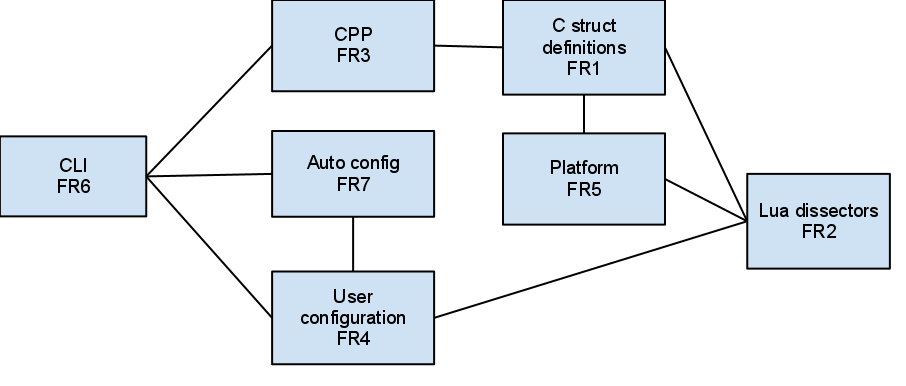
\includegraphics[width=\textwidth]{./planning/img/requirement_relationship}
	\caption{Relationship Between Requirements \label{fig:req:relationship}}
\end{figure}

%------------------
\section{Use Cases}
%------------------
\label{sec:req:usecases}
This sections contains use case diagrams for our two actors, and detailed
textual use cases for these diagrams.

\subsection{Actors}
%------------------
An actor specifies a role played by an external person or thing that interact
with our \gls{utility}. We have three types of actors to consider. First is the
primary actor, that uses the \gls{utility} to generate \glspl{dissector} from 
\Gls{c} header-files. A secondary actor is the user who configures the
\gls{utility} to change the output of it. Finally, we have an offstage actor, which
does not use our \gls{utility} himself, but uses the outputted \glspl{dissector} in \Gls{wireshark}.

We have defined two use case actors for our \gls{utility}. The customer has specified
that the offstage actor, called developer, is the most important actor.
\begin{description}
	\item[Developer] User of the generated \Gls{wireshark} \glspl{dissector}, offstage actor
	\item[Administrator] User and configurer of \gls{utility}, primary and secondary actor
\end{description}

\subsection{Use Case Diagrams}
%-----------------------------
\hyperref[fig:req:ucadm]{Figure \ref*{fig:req:ucadm}} shows the use case
diagram for the administrator, and \autoref{fig:req:ucdev} is the use case
diagram for the developer.
\begin{figure}[htbp]
	\center
	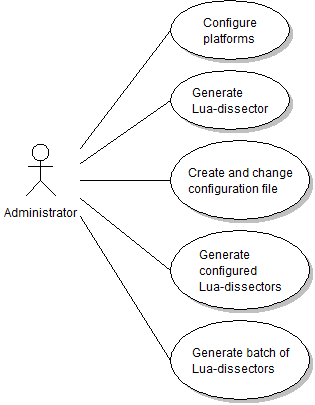
\includegraphics[width=0.6\textwidth]{./planning/img/uc_administrator}
	\caption{Use Case Diagram: Administrator\label{fig:req:ucadm}}
\end{figure}

\begin{figure}[htbp]
	\center
	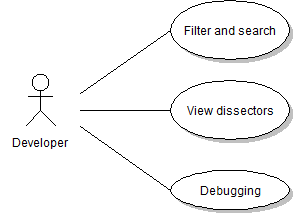
\includegraphics[width=0.6\textwidth]{./planning/img/uc_developer}
	\caption{Use Case Diagram: Developer\label{fig:req:ucdev}}
\end{figure}

\subsection{Textual Use Cases}
%-----------------------------
Here each of the use cases are described textually.

\begin{table}[htbp] \footnotesize \center
\caption{Filter and search textual use case\label{tab:textual:filterandsearch}}
\noindent\makebox[\textwidth]{%
\begin{tabularx}{1.2\textwidth}{l X}
	\toprule
	 & 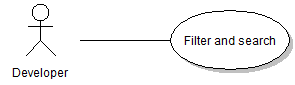
\includegraphics[scale=0.8]{./planning/img/uc_filterandsearch} \\
	\toprule
	Element & Description\\
	\midrule
	Use case name & Filter and search on attributes\\
	Goal & The developer wants the correct set of results based on the search phrase \\
	Summary & The developer would like to filter and search on attributes in the packets displayed in Wireshark \\
	Preconditions & Wireshark need to be running with dissectors. \\
	Postconditions & Wireshark display the results.\\
	\midrule
	\multirow{3}{*}{Flow of Events} & 1. The developer selects the search field in Wireshark's GUI.  \\
	& 2. The user types in a search phrase. \\
	& 3. Wireshark will present the search results that match the query. \\
	\midrule
	Exceptions & None. \\
	\bottomrule
\end{tabularx}}
\end{table}

\begin{table}[htbp] \footnotesize \center
\caption{View dissector textual use case\label{tab:textual:viewdissector}}
\noindent\makebox[\textwidth]{%
\begin{tabularx}{1.2\textwidth}{l X}
	\toprule
	 & 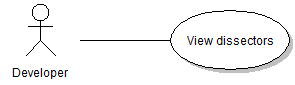
\includegraphics[scale=0.8]{./planning/img/uc_viewdissectors} \\
	\toprule
	Element & Description\\
	\midrule
	Use case name & View the dissectors in Wireshark\\
	Goal & View structs correctly dissected in Wireshark\\
	Summary & The developer would like to dissect a structs and have the members and values displayed in Wireshark by using the dissectors in Wireshakrs plugin folder.\\
	\multirow{2}{*}{Preconditions}& 1. The developer have Wireshark running with dissectors. \\
	& 2. The dissector for a struct will dissect it correctly, according to the initial internal structure of the struct. \\
	Postconditions & Wireshark display the struct with the correct structure and values.\\
	\midrule
	\multirow{3}{*}{Flow of Events} & 1. The developer selects a struct message in Wireshark. \\
	& 2. Wireshark calls the correct dissector and dissects the selected message. \\
	& 3. Wireshark displays the members and values of the selected message. \\
	\midrule
	\multirow{2}{*}{Exceptions} & 1. The correct dissector for a struct might not exist in Wiresharks plugin folder, making it impossible to dissect the message. \\
	& 2. more? \\
	\bottomrule
\end{tabularx}}
\end{table}

\begin{table}[htbp] \footnotesize \center
\caption{Debugging textual use case\label{tab:textual:debugging}}
\noindent\makebox[\textwidth]{%
\begin{tabularx}{1.2\textwidth}{l X}
	\toprule
	 & 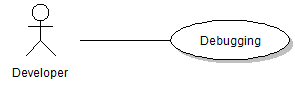
\includegraphics[scale=0.8]{./planning/img/uc_debugging} \\
	\toprule
	Element & Description\\
	\midrule
	Use case name & Filter and search on attributes\\
	Goal & The user wants the correct set of results based on the search phrase \\
	Summary & The user would like to filter and search on attributes in the packets displayed in Wireshark \\
	Preconditions & The user have Wireshark running with dissectors. \\
	Postconditions & Wireshark display the results.\\
	Flow of Events & The user selects the search field in Wireshark's API and types in a search phrase, then Wireshark will present the search results that match the query. \\
	Exceptions & N/A \\
	\bottomrule
\end{tabularx}}
\end{table}

\begin{table}[htbp] \footnotesize \center
\caption{Configure platforms textual use case\label{tab:textual:configureplatforms}}
\noindent\makebox[\textwidth]{%
\begin{tabularx}{1.2\textwidth}{l X}
	\toprule
	 & 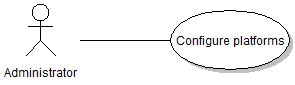
\includegraphics[scale=0.8]{./planning/img/uc_configureplatform} \\
	\toprule
	Element & Description\\
	\midrule
	Use case name & Filter and search on attributes\\
	Goal & The administrator would like to filter and search on attributes in the packets displayed in Wireshark \\
	Summary & \\
	Preconditions & The user have Wireshark running with dissectors. \\
	Postconditions & Wireshark display the results.\\
	Flow of Events & The user selects the search field in Wireshark's API and types in a search phrase, then Wireshark will present the search results that match the query. \\
	Exceptions & N/A \\
	\bottomrule
\end{tabularx}}
\end{table}

\begin{table}[htbp] \footnotesize \center
\caption{Generate Lua dissector textual use case\label{tab:textual:generatelua}}
\noindent\makebox[\textwidth]{%
\begin{tabularx}{1.2\textwidth}{l X}
	\toprule
	 & 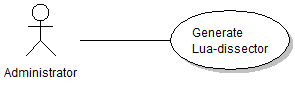
\includegraphics[scale=0.8]{./planning/img/uc_generatelua} \\
	\toprule
	Element & Description\\
	\midrule
	Use case name & Filter and search on attributes\\
	Goal & The user would like to filter and search on attributes in the packets displayed in Wireshark \\
	Summary & \\
	Preconditions & The user have Wireshark running with dissectors. \\
	Postconditions & Wireshark display the results.\\
	Flow of Events & The user selects the search field in Wireshark's API and types in a search phrase, then Wireshark will present the search results that match the query. \\
	Exceptions & N/A \\
	\bottomrule
\end{tabularx}}
\end{table}

\begin{table}[htbp] \footnotesize \center
\caption{Create and change configuration file textual use case\label{tab:textual:configure}}
\noindent\makebox[\textwidth]{%
\begin{tabularx}{1.2\textwidth}{l X}
	\toprule
	 & 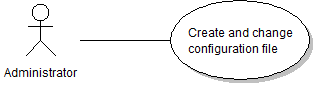
\includegraphics[scale=0.8]{./planning/img/uc_configurate} \\
	\toprule
	Element & Description\\
	\midrule
	Use case name & Filter and search on attributes\\
	Goal & The user would like to filter and search on attributes in the packets displayed in Wireshark \\
	Summary & \\
	Preconditions & The user have Wireshark running with dissectors. \\
	Postconditions & Wireshark display the results.\\
	Flow of Events & The user selects the search field in Wireshark's API and types in a search phrase, then Wireshark will present the search results that match the query. \\
	Exceptions & N/A \\
	\bottomrule
\end{tabularx}}
\end{table}

\begin{table}[htbp] \footnotesize \center
\caption{Generate configured Lua-dissectors textual use case\label{tab:textual:generateconfiglua}}
\noindent\makebox[\textwidth]{%
\begin{tabularx}{1.2\textwidth}{l X}
	\toprule
	 & 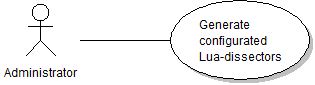
\includegraphics[scale=0.8]{./planning/img/uc_generateconfiglua} \\
	\toprule
	Element & Description\\
	\midrule
	Use case name & Filter and search on attributes\\
	Goal & The user would like to filter and search on attributes in the packets displayed in Wireshark \\
	Summary & \\
	Preconditions & The user have Wireshark running with dissectors. \\
	Postconditions & Wireshark display the results.\\
	Flow of Events & The user selects the search field in Wireshark's API and types in a search phrase, then Wireshark will present the search results that match the query. \\
	Exceptions & N/A \\
	\bottomrule
\end{tabularx}}
\end{table}

\begin{table}[htbp] \footnotesize \center
\caption{Generate batch of Lua dissectors textual use case\label{tab:textual:luabatch}}
\noindent\makebox[\textwidth]{%
\begin{tabularx}{1.2\textwidth}{l X}
	\toprule
	 & 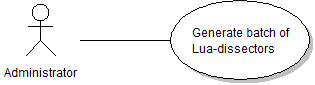
\includegraphics[scale=0.8]{./planning/img/uc_luabatch} \\
	\toprule
	Element & Description\\
	\midrule
	Use case name & Filter and search on attributes\\
	Goal & The user would like to filter and search on attributes in the packets displayed in Wireshark \\
	Summary & \\
	Preconditions & The user have Wireshark running with dissectors. \\
	Postconditions & Wireshark display the results.\\
	Flow of Events & The user selects the search field in Wireshark's API and types in a search phrase, then Wireshark will present the search results that match the query. \\
	Exceptions & N/A \\
	\bottomrule
\end{tabularx}}
\end{table}

\section{User Stories}
To make it easier to implement the requirements, there have been written user stories. The user stories describes how the requirements should be implemented, and was written in each sprint planning meeting. The user stories that are written can be found in the sprint design for each of the sprint. \autoref{tab:us:template} shows an template of an user story.

\begin{table}[htbp] \footnotesize \center
\caption{User Story Template\label{tab:us:template}}
\noindent\makebox[\textwidth]{%
\begin{tabularx}{1.2\textwidth}{l X}
\toprule
Header & Value \\
\midrule
ID & ID for the user stories, written like USxx. \\
Requirements & The requirement that the user story descripbes. \\
What & Description of what the user want to achieve.\\
How & Description of how the requirement should be implemented. \\
Result & What the result is after the implementation. \\
\bottomrule
\end{tabularx}}
\end{table}



\section{Product Backlog}
%------------------------
\label{sec:prodbacklog}
The complete product backlog can be seen in \autoref{tab:prodbacklog}.
Optional requirements which we did not implement are listed in
\autoref{tab:prodbacklog2}. These optional requirements are described
in \autoref{sec:eval:furtherdev}.

\begin{table}[htbp] \small \center
\caption{Optional Requirements Estimates\label{tab:prodbacklog2}}
\begin{tabularx}{\textwidth}{l X c}
	\toprule
	Req. & Description & Est. Hours \\
	\midrule	
	FR2-F & Display if struct member contains uninitialized memory & 8 \\
	FR6-D & Do not regenerate dissectors across multiple runs & 2 \\
	FR7-A & Find struct descriptions from Doxygen comments & 20 \\
	FR7-B & Find configuration of \#define enums from header files & 20 \\
	\midrule
	& Total & 50 \\
	\bottomrule
\end{tabularx}
\end{table}

%\begin{table}[htbp] \footnotesize \center
\begin{table}[htbp] \small \center
\caption{Product Backlog\label{tab:prodbacklog}}
\noindent\makebox[\textwidth]{%
\begin{tabularx}{1.13\textwidth}{l X c c c}
	\toprule
	& & & \multicolumn{2}{c}{Hours} \\
	\cmidrule(r){4-5}
	Req. & Description & Sprint & Est. & Act. \\
	\midrule
	FR1 & Read basic \Gls{c} \gls{struct} definitions & & \textbf{52}  & \textbf{51}  \\
	FR1-A & Support data types: \gls{int}, \gls{float}, \gls{char} and \gls{boolean} & SP1 & 24 & 21 \\
	FR1-B & Support \glspl{member} of type \gls{enum} & SP2 & 6 & 5 \\
	FR1-C & Support \glspl{member} of type \gls{struct} & SP2 & 7 & 3.5 \\
	FR1-D & Support \glspl{member} of type \gls{union} & SP3 & 5 & 6 \\
	FR1-E & Support \glspl{member} of type \gls{array} & SP2 & 7 & 12 \\
	FR1-F & Detect \glspl{struct} with same name & SP2 & 3 & 3.5 \\
	\addlinespace
	FR2 & Generate \Gls{wireshark} \glspl{dissector} in \Gls{lua} & & \textbf{69} &  \textbf{59.5} \\
	FR2-A & Display simple \glspl{struct} & SP1 & 28 & 25 \\
	FR2-B & Support display of \glspl{struct} within \glspl{struct} & SP2 & 11 & 15 \\
	FR2-C & Support \Gls{wireshark} filter and search on attributes & SP3 & 3 & 1.5 \\
	FR2-D & Recognize invalid values for a \gls{struct} \gls{member} & SP1 & 22 & 15 \\
	FR2-E & Guess \glspl{dissector} from packet size & SP4 & 5 & 3\\
    \addlinespace
	FR3 & Support \Gls{c} \gls{preprocessor} directives and macros & & \textbf{24} &  \textbf{7.5}\\
	FR3-A & Support \gls{include} & SP1 & 8 & 2 \\
	FR3-B & Support \gls{define} and \gls{if} & SP1 & 11 & 3 \\
	FR3-C & Support \verb+_WIN32+, \verb+_WIN64+, \verb+__sparc+ etc & SP3 & 5 & 2.5 \\
	\addlinespace
	FR4 & Support user configuration & & \textbf{91} & \textbf{71}\\
	FR4-A & Support valid ranges for \gls{struct} \glspl{member} & SP1 & 30 & 15 \\
	FR4-B & Support custom \Gls{lua} files for specific protocols & SP3 & 10 & 7.5 \\
	FR4-C & Support custom handling of specific data types & SP2 & 6 & 5 \\
	FR4-D & Support specifying the ID of \glspl{dissector} & SP2 & 7 & 9 \\
	FR4-E & Support various \gls{trailers} (other registered protocols) & SP2 & 18 & 15 \\
	FR4-F & Support \glspl{enumerated named value} & SP2 & 5 & 6.5 \\
	FR4-G & Support bit strings & SP2 & 10 & 11.5 \\
	FR4-H & Automatic generation of placeholder configuration & SP4 & 1 & 0.5\\
	FR4-I & Support specifying the size of unknown struct members & SP4 & 4 & 1\\
	\addlinespace
	FR5 & Handle input which size and \gls{endian} depends on platform & & \textbf{40} & \textbf{23.5} \\
	FR5-A & Flags specified for each platform & SP3 & 8 & 11 \\
	FR5-B & \Glspl{dissector} support memory alignment & SP3 & 12 & 6.5 \\
	FR5-C & \Glspl{dissector} support both little and big \gls{endian} & SP3 & 6 & 4 \\
	FR5-D & \Glspl{dissector} support different sizes from flags & SP3 & 14 & 2 \\	
    \addlinespace
	FR6 & Support parameters from command line & & \textbf{51} & \textbf{24}\\
	FR6-A & Support parameter for \Gls{c} \gls{header} file & SP1 & 9 & 9 \\
	FR6-B & Support parameter for configuration file & SP1 & 28 & 8 \\
	FR6-C & Support batch processing of \Gls{c} \gls{header} and configuration & SP2 & 7 & 4.5 \\
	FR6-E & Support C \#defines and --Include from CLI & SP4 & 1 & 1 \\
	FR6-F & Only generate dissectors for structs with valid ID & SP4 & 4 & 1.5 \\
	\midrule
	& Total & & 327 & 236.5 \\
    \bottomrule
\end{tabularx}}
\end{table}	


%==================
\chapter{Test Plan}
%==================
This chapter presents the test plan for our solution. The test plan is based on
the standards set by the IEEE829-1998 standard for software testing\cite{IEEE829}, but with a
few changes to better fit with our project. The purpose of this plan is to have
a structured way of performing tests, as well as providing the developers with
a list of specific component-behaviors. The tests will be based on functional as
well as non-functional requirements, deterring architectural drift and
enforcing our design plans for the system.


%----------------------------
\section{Methods for Testing}
%----------------------------
When it comes to software testing, we have two different types of tests available, namely Black box and white box tests. This section is dedicated to the discussion of these two testing methodologies.


%--------------------------
\subsection{White box Testing}
%--------------------------
White box testing is a method of software testing where you test internal structures or modules of an application, as opposed to its functions. White box testing requires the tester to have an internal perspective of the system, as well as sufficent programming skills. As the \gls{utility} was required to be able to function with a variety of different input, as well as being used as a debugging tool itself, we chose to have every developer on the team write unit tests for their own code, and then have someone else on the team do the testing of their code in order to ensure correctness. Also, in order to get a proper overview over what and how many parts of the system that are covered by unit tests, the team decided to use a tool for measuring code coverage.

\subsubsection{Attest}
As a tool for creating white box unit tests the team decided to use the Attest testing framework for python code. To create unit tests using Attest, you start off by importing Tests, assert\_hook and optionally contexts from attest. You then create a variable and initialize it to an instance of Tests, which is the variable that will contain list functions that each constitutes one test that is to be run. To feed your test instance with functions for testing you then have to mark these functions with a decorator and feed it the .tests function of the Tests instance. After creating a unit test in this fashion you can run all of your unit tests through Attest from the command line by typing ''python -m attes''. This runs all of your unit tests through Attest and returns a message telling the user how many assertions failed as well as what input made them fail. For more information read the user documentation of Attest. 

\subsubsection{Coverage}
As a tool for calculating code coverage the team decided to use Coverage, which is a tool for measuring code coverage in python projects. In order to run Coverage from the command line with the tests for this utility you would have to first navigate to the folder where you installed CSjark, before typing ''Coverage run -m attest''. This generates a file that will be used to Coverage for generating a html table displaying the coverage. In order to create this html table you would then have to type ''coverage html'', which generates a folder named htmlcov. This htmlcov folder again contains a file named index.html that contains a html table describing which parts of the system underwent testing and their code coverage.


%--------------------------
\subsection{Black Box Testing}
%--------------------------
Black box testing is a method of software testing where you test the functionality of a system, as opposed to its internal structures. Black box testing does in general not require the tester to have any intimate knowledge about the system or any of the programming logic that went into making it. Black box test cases are built around the specifications and requirements of a system, i.e its functional and in some cases non-functional requirements. The team decided to use black box testing for both the functional and non-functional requirements of the \gls{utility}, as the customer had already expressed thoughts on extending and understanding the non-functional parts of the \gls{utility} themselves. 

%--------------------------------------------
\section{Non-Functional Requirements}
%---------------------------------------------
As evaluating the non-functional requirements of a system through its source code is very difficult it was decided that we should create test cases for them the same way we created black box test cases. Some of these tests would also require the team to have more manpower or resources than what can be expected by a group of students. It was therefore also decided that we would ask the customer for help regarding the testing of some of the non-functioanl requirements. These testcases would then be designed according to the wishes of the customer and what resources they were able to supply us with.

%------------------------------
\section{Templates for Testing}
%------------------------------
\autoref{tab:testcase} , \autoref{tab:testreport} and \autoref{tab:TestCoverageReport} are templates we will be
using for testing purposes.

In order to standarize the testing process, the team decided on making templates for both the test cases themselves and for reporting their results. The ones responsible for testing were given the task of not only creating and running the testcases themselves, but also adhering to the standards set in this document.

\autoref{tab:testcase} shows the template for each test case. All of the test cases written for the \gls{utility} will be in this format, and executed according to this document.

\begin{table}[htb] \small \center
\caption{Test case template \label{tab:testcase}}
\begin{tabular}{l l}
	\toprule
	Header & Description \\
	\midrule
	Description & Description of requirement \\
	Tester & Team member responsible for the test \\
	Prerequisites & Conditions that needs to be fulfilled before starting the test \\
	Feature & Feature to test \\
	Execution & Steps to be executed in the test \\
	Expected result & The expected output of the test \\
	\bottomrule
\end{tabular}
\end{table}

\autoref{tab:testreport} shows the template for reporting the result of each test case.

\begin{table}[htb] \small \center
\caption{Test report template \label{tab:testreport}}
\begin{tabular}{l l}
	\toprule
	Header & Description \\
	\midrule
	Description & Description of requirement \\
	Tester & Team member responsible for the test \\
	Date & The date the testing took place \\
	Result & The success or failure of the test, and a comment on the result if needed \\
	\bottomrule
\end{tabular}
\end{table}

\autoref{tab:TestCoverageReport} shows the template for reporting code coverage.

\begin{table}[!htb]\footnotesize\center
	\caption{Code Coverage Report Template\label{tab:TestCoverageReport}}
	\begin{tabular}{l l l l l}
		\toprule
		Module & Statements & Missing & Excluded & Coverage\\
		\midrule
		module 1 & Statements ran & Statements not ran  & Excluded statements & Percent code coverage\ \\
		... & ... & ... & ... & ... \\
		module n & Statements ran & Statements not ran & Excluded statements  & Percent code coverage \\
		\bottomrule
		Total & Statements ran & Statements not ran & Excluded statements & Percent code coverage \\
		\bottomrule
	\end{tabular}
\end{table}


%-----------------------
\section{Test Criterias}
%-----------------------
An item will be considered to have passed a test if the actual result from the test matches the expected result from the test. An item will be considered to have failed the test if the output varies from the expected result. If there are any specifics as to why the test passed/failed, which needs to be discussed, they will be listed as a comment to the result


%---------------------------------
\section{Testing Responsibilities}
%---------------------------------
Each team member is responsible for writing their own unit tests while the test leader is responsible for the quality of the test plan and the tests. The tests will mainly not be executed by the same developers who wrote the code that is to undergo testing, but by others in the testing team with as little ownership of the code as possible. 

%---------------------
\section{Changelog}
%----------------------

\subsection{Sprint 1}
%----------------------
During sprint 1, it became apparent that the customers would not be able to supply the team with any real traffic data to use for testing. The testing team therefore decided to use a hex-editor to generate their own data \glspl{packet} with the \Gls{c}-\glspl{struct} that would be used for testing the \gls{utility}. This is done by manually writing the hex values for the individual bytes in a pcap \gls{packet}, where the first byte indicates the version number, the second byte indicates the flag value of the \gls{packet} and where the third and fourth byte indicates the message ID. The rest of the bytes in the \gls{packet} then contain the \gls{member} values of whatever \gls{struct} was associated with the \gls{packet}'s message ID.

During the sprint, it also became apparent that \Gls{wireshark} would be able to provide the developers and testers with feedback on syntax and user errors on both the \glspl{dissector} created by the \gls{utility}, as well as the traffic used for testing. This is done by \Gls{wireshark} crashing and/or providing the team with error messages related to the code in which the \gls{dissector} is faulty. There will also be displayed a warning or error message with the generated traffic-data if there are any faults with them. The team was therefore able to use \Gls{wireshark} in assisting them in creating correct code early on before writing unit tests.   

\subsection{Sprint 2}
%----------------------
As of sprint 2, it was decided that the team should use an automated tool for calculating code coverage. Code coverage is a measure describing the actual amount of, and which code that undergoes unit testing. As code coverage inspects code directly, it is considered a form of white box testing. In this project it will be used to ensure that an as big part as possible of the system actually undergoes testing, and that the unit tests associated with the different modules of the \gls{utility} actually tests what they are supposed to. It was also added as a goal to have at least 80\% at the end of the project, where the testers and developers would aim to increase the amount of code coverage from each previous sprint.

\subsection{Sprint 3}
%----------------------
During sprint 3, it was suggested that the team should create a \Gls{c}-program that generates \glspl{hex dump} that were to be used for generating traffic to test the \gls{utility} with. It was therefore decided that the team would create such a program to generate data for the bigger and more complex \Gls{c}-\gls{header} files that could have a dozen of \gls{struct}-\glspl{member} of various types. This would help the team to be able to generate more test traffic for the most complex \glspl{header} without having to spend much extra time manually writing down the hex values of each \gls{struct} \gls{member}.

\subsection{Sprint 4}
%----------------------


%==================================
\chapter{Architectural Description}
%==================================
This chapter introduces the architectural documents pertaining to our solution. The team followed the definition of software architecture defined by Len Bass, Paul Clements and Rick Kazman: "The software architecture of a program or computing
system is the structure of structures of the system, which comprise software elements, the externally visible properties of those elements, and the relationships between them."\cite{Bass2003}

The purpose of this document is to describe our architecture in a structured way so that it can be used not only by the team, but also as an aid for other stakeholders who are trying to understand the system.


%------------------------------
\section{Architectural Drivers}
%------------------------------
This section is dedicated to the discussion of the architectural drivers.
The team has chosen Modifiability and Testability as the quality attributes for this utility. 

The reason for using Modifiability is that the development team are not going to be the ones updating or maintaining the utility after the completing the project. It is therefore important that the code is easy to understand, well documented and easy to modify. This will make it easier for our customer to later modifiy or extend the utility.

Testability is important since the utility will be used for debugging by the customer.  Since it is not possible for the team to test the dissectors in a real environment, it will be more important to focus on testing. This is to ensure that the final product is working correctly.

\subsection{Testability Tactics}
%-------------------------------
The goal of using testability tactics is making it easier to test the system after finishing an increment of the software development. 

\subsubsection{Specialize Access Routes/Interfaces}
Using a specialized testing interface makes it possible to specify values for a component independently from its normal execution. This will in turn make it possible to test parts of an unfinished module as well as making it easier to get a clear overview over what data is flowing through individual parts of the system.

\subsection{Modifiability Tactics}
%---------------------------------
The goal of using modifiability tactics are to make it easier to extend and modify the software during the development and after the completion of a working product.

\subsubsection{Anticipate Expected Changes}
By trying to anticipate expected changes it is possible to make it easier for modules to be extended with new functionality later. It also makes it easier for the developers to anticipate the different ranges of input the modules are about be able to process.

\subsubsection{Limit Possible Options}
By limiting the range of possible modifications to the system it becomes easier to generalize the structure of different modules. This will in turn make it easier to constrict the wide ranging effect of new modifications to the system, giving the developers a clearer view over what a given change will actually do to the system.

\subsubsection{Generalizing Modules}
Generalizing the modules of a system makes it possible to reuse older modules when doing modifications to the system. The more general a module, the more likely it is that a needed change to the system can be implemented by just adjusting the input to the system rather than having to modify existing or creating new modules.

\subsubsection{Restrict Communication Paths}
By restricting the number of modules that are able to collect data from a specific module, the less dependent the entire system becomes of that specific module. This makes it easier to swap out existing modules with new ones without having to make many widespread changes to the entire system.

\subsubsection{Using Configuration Files}
By using configuration files, it is possible to change the behaviour of the system without having to do any changes to its code.

\subsection{Business Requirements}
%---------------------------------
\begin{itemize}
\item The utility must be delivered on time as it is not possible for the developers to continue the development after the deadline
\item The ability for the utility to be able to create dissectors for C-structs in header files used by Thales
\item The ability for the utility to create dissectors that run on all of the platforms used by Thales and their customers
\item The ability for wireshark to be able to use the generated dissectors to display the values in c-structs passed through the system.
\end{itemize}


%------------------------------
\section{Architectural Patters}
%------------------------------
This section presents the different architectural patterns used in the utility

\subsection{Pipe and Filter}
%---------------------------
The pipe and filter architectural pattern consists of a stream of data which in turn is processed sequentially by several filters in such a fashion that the output of one filter becomes the input of the other. It is a very flexible yet robust way of processing data, with support for adding more filters if needed for future applications and processes.

\begin{figure}[htb]
	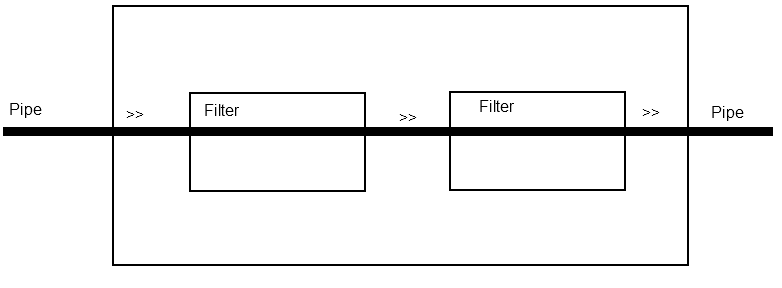
\includegraphics[width=\textwidth]{./planning/img/PipeAndFilter}
	\caption{Pipe and Filter Pattern\label{fig:pipefilter}}
\end{figure}


%----------------------------
\section{Architectural Views}
%----------------------------
This section describes three different views: Logival view, process view and deployment view.

\subsection{Logical View}
%------------------------
This view shown in \autoref{fig:logicalview}. Command line takes the arguments for header file and configuration file as a string. The arguments are parsed in the command line parser. Header file is sent to ''C preprocessor \& C parser", the C header file is loaded and parsed by the C parser, whcih generates a parsing tree. Command line also call Configuration, which load the configuration file. The configuration will parse the configuration file and create configuation rules. The Lua script generator will generate a Lua script from the parsing tree and the config rules.

\begin{figure}[htb]
	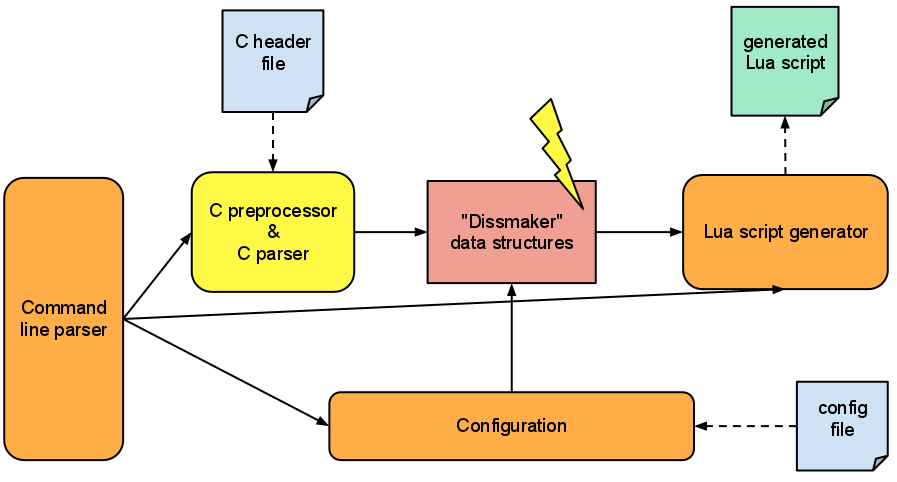
\includegraphics[width=\textwidth]{./planning/img/overall_design}
	\caption{Overall Architecture\label{fig:logicalview}}
\end{figure}


%---------------------
\subsection{Process View}
%---------------------
\autoref{fig:processview} shows the process view for our utility. Csjark takes header and config files as input and then uses the config and cparser to parse the files. CSjark then uses the cparser to find the structs in the header file and then creates dissectors for them. These dissectors are then written to a file and CSjark then reports to the user by sending a message to the command line.

\begin{figure}[htb]
	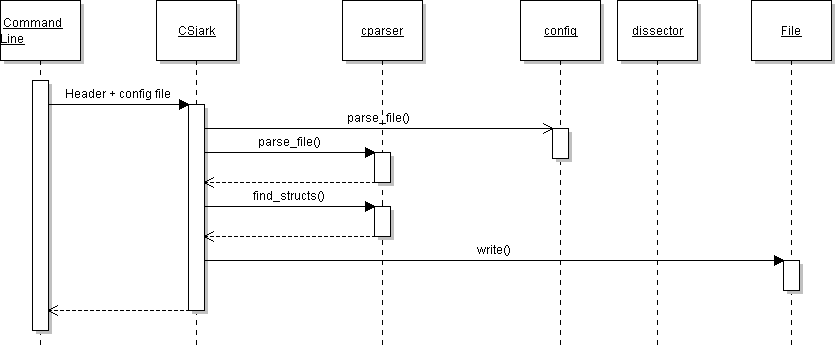
\includegraphics[width=\textwidth]{./planning/img/SequenceDiagram}
	\caption{Data flow during regular execution\label{fig:processview}}
\end{figure}


%------------------------
\subsection{Deployment View}
%------------------------
\autoref{fig:deployment} shows the deployment diagram for this project. Csjark takes header- and config-files as input, and generates Lua-scripts. The Lua-scripts are used for dissectors in Wireshark.

\begin{figure}[htb]
	\includegraphics[width = \textwidth]{./planning/img/Deployment}
	\caption{Deployment View\label{fig:deployment}}
\end{figure}


%--------------------------------
\section{Architectural Rationale}
%--------------------------------
The team decided to use the pipe and filter pattern as the architects felt that it was the only architectural pattern that would benefit the utility without having to make it needlessly complex. The utility was supposed to take header files as input and then process the data from them several times until the end result was a list of structs and members that could be used to make dissectors for wireshark. This seemed like an excellent application to use the pipe and filter pattern with, as it would then be easy to add new filters to the header file for future increments of the development cycle without having to rewrite what had already been implemented in previous sprints.

For the views the team decided to use a logical view, process view and deployment view. These views were chosen because the architects of the utility felt that these views alone could represent the system sufficently without creating too much overhead for the readers of the document. The logical view supplies the reader with a more in depth view of what the system is comprised of, which is useful for developers who need to figure out the workings of the system. The process view also seemed important for the developers and the testers of the utility, as it provides the reader with a more proper overview of the dataflow in the system. This makes it a lot easier to see which modules are run when and which external calls that dictates their behaviour. Lastly a deployment view was chosen to make it more clear for the reader of the document what the utility really produces as output and what other external applications it has to cooperate with. 




%#########
% Sprints
%#########
\part{Sprints}
%=================
\chapter{Sprint 1}
%=================

\section{Back log}
%-----------------
\begin{table}[ht] \small \center
\caption{Sprint 1 Requirement FR7-A}
\begin{tabular}{l l c}
	\toprule
	Requirement & Task & Hours \\
	\midrule
	\multirow{4}{5cm}{Command line shall support parameters for c-header file} & Design & 1 \\
	& Implementation & 2 \\
	& Testing & 2 \\
	& Documentation & 4 \\
	\bottomrule
\end{tabular}
\end{table}

\begin{table}[ht] \small \center
\caption{Sprint 1 Requirement FR1-A}
\begin{tabular}{l l c}
	\toprule
	Requirement & Task & Hours \\
	\midrule
	\multirow{4}{5cm}{The utility must support the following basic data types: int, float, char and boolean} & Design & 4 \\
	& Implementation & 8 \\
	& Testing & 8 \\
	& Documentation & 4 \\
	\bottomrule
\end{tabular}
\end{table}

\begin{table}[ht] \small \center
\caption{Sprint 1 Requirement FR2-A}
\begin{tabular}{l l c}
	\toprule
	Requirement & Task & Hours \\
	\midrule
	\multirow{4}{5cm}{The dissector shall be able to display simple structs} & Design & 4 \\
	& Implementation & 8 \\
	& Testing & 8 \\
	& Documentation & 8 \\
	\bottomrule
\end{tabular}
\end{table}

\begin{table}[ht] \small \center
\caption{Sprint 1 Requirement FR3-A}
\begin{tabular}{l l c}
	\toprule
	Requirement & Task & Hours \\
	\midrule
	\multirow{4}{5cm}{The utility shall support \#include} & Design & 2 \\
	& Implementation & 2 \\
	& Testing & 2 \\
	& Documentation & 2 \\
	\bottomrule
\end{tabular}
\end{table}

\begin{table}[ht] \small \center
\caption{Sprint 1 Requirement FR3-B}
\begin{tabular}{l l c}
	\toprule
	Requirement & Task & Hours \\
	\midrule
	\multirow{4}{5cm}{The utility shall support \#define and \#if} & Design & 1 \\
	& Implementation & 2 \\
	& Testing & 6 \\
	& Documentation & 2 \\
	\bottomrule
\end{tabular}
\end{table}

\begin{table}[ht] \small \center
\caption{Sprint 1 Requirement FR7-B}
\begin{tabular}{l l c}
	\toprule
	Requirement & Task & Hours \\
	\midrule
	\multirow{4}{5cm}{Command line shall support for configuration file} & Design & 8 \\
	& Implementation & 8 \\
	& Testing & 8 \\
	& Documentation & 4 \\
	\bottomrule
\end{tabular}
\end{table}

\begin{table}[ht] \small \center
\caption{Sprint 1 Requirement FR4-A}
\begin{tabular}{l l c}
	\toprule
	Requirement & Task & Hours \\
	\midrule
	\multirow{4}{5cm}{Configuration must support valid ranges for struct members} & Design & 6 \\
	& Implementation & 8 \\
	& Testing & 8 \\
	& Documentation & 8 \\
	\bottomrule
\end{tabular}
\end{table}

\begin{table}[ht] \small \center
\caption{Sprint 1 Requirement FR2-D}
\begin{tabular}{l l c}
	\toprule
	Requirement & Task & Hours \\
	\midrule
	\multirow{4}{5cm}{The dissector shall be able to recognize invalid values for a struct member} & Design & 4 \\
	& Implementation & 6 \\
	& Testing & 8 \\
	& Documentation & 4 \\
	\bottomrule
\end{tabular}
\end{table}

\begin{table}[ht] \small \center
\caption{Sprint 1 Requirements}
\begin{tabularx}{\textwidth}{l l X c c}
	\toprule
	& & & \multicolumn{2}{c}{Hours} \\
	\cmidrule(r){4-5}
	\# & Req. & Description & Est. & Act. \\
	\midrule
	1 & FR7-A & Command line shall support parameters for c-header file & 9 & -\\
	\addlinespace
	2 & FR1-A & Support basic data types: int, float, char, boolean & 24 & -\\	
	\addlinespace
	3 & FR2-A & The dissector shall be able to display simple structs & 28 & -\\
	\addlinespace
	4 & FR3-A & The utility shall support \#include & 8 & -\\
	\addlinespace
	5 & FR3-B & The utility shall support \#define and \#if & 11 & -\\	
	\addlinespace
	6 & FR7-B & Command line shall support for configuration file & 28 & -\\
	\addlinespace
	7 & FR4-A & Support valid ranges for struct members & 30 & -\\
	\addlinespace
	8 & FR2-D & Recognize invalid values for a struct member & 22 & -\\
	\midrule
	 & & Total: & 160 & - \\
	 \bottomrule
\end{tabularx}
\end{table}

\begin{table}[ht] \small \center
\caption{Sprint 1 Timetable}
\begin{tabularx}{\textwidth}{X c c}
	\toprule
	 & \multicolumn{2}{c}{Hours} \\
	\cmidrule(r){2-3}
	 Description & Est. & Act. \\
	\midrule
	Design & 30 & -\\
	\addlinespace
	Implementation & 44 & -\\
	\addlinespace
	Testing & 50 & -\\
	\addlinespace
	Documentation & 36 & -\\
	\midrule
	Total: & 160 & - \\
\end{tabularx}
\end{table} 


%=================
\chapter{Sprint 2}
%=================

%-------------------
\section{Pre-sprint}
%-------------------
Sprint 1 gave the desired result, but the team was not satisfied with the way the Scrum process was conducted, especially the sprint planning. In sprint 1 retrospect we decided to conform more to, in our mind, proper Scrum. Applying experience and advice from the first sprint, to get a better process. 

This planning meeting we will try to have more descriptive work items in the sprint backlog. This will ease the process of design, implementation, testing and documentation of the utility, and we do not have to redo any parts that will end up in the report in order to assist the reader. We focus on good user stories to ensure that the elements are low enough level.


%------------------------
\section{Sprint Planning}
%------------------------
The first sprint resulted in a solid core for the utility. During the next sprint iteration, the core will be extended with more advanced functionality. After this sprint, the utility will have most of the functionalities it need to work in a real environment, and will probably be able to aid Thales in some of their operations.

Not yet understanding the complexity of all the requirements in the sprint backlog, the team ended in an uncertain person-hours estimate for some work objects. Time will show if we understood the complexity and assigned enough hours to implement it. The more complex, but not so critical functionalities will be part of sprint 3 and 4.   

\subsection{Duration}
%--------------------
According to the work breakdown structure, \autoref{tab:wbs}, the planning meeting of the second sprint should have been conducted the 5th of October. After a request from the customer to see our planning for the second sprint at the weekly customer meeting, which was scheduled to be before our planning meeting the same day, we decided to advance the planning to the 4th of October. This is to maintain the good relationship to the customer and submit to their preference.

The sprint started with the planning meeting the 4th of October and our work started the following day. The sprint duration is 14 days, and will end the 18th of October with a review meeting.  

\subsection{Sprint Goal}
%-----------------------
The second sprint will build on the core created in the first sprint. During the sprint we will extend the functionality with more comprehensive and advanced features. Most of the requirements we intend to fulfill in this sprint had to be done subsequent to the first sprint, because the structure and design of the core had to be in place first. The requirements that are selected for this sprint is a natural advancement on the way to make the utility that the customer wants. 

One of the most crucial functions to work in a real environment, is the support for nested header-files. The handling of the \#include-statement gives the utility this feature. The goal of the sprint is to implement the \#include and mainly to have support for enums, bit streams, endianness and batch mode. 

\subsection{Back Log}
%--------------------
\label{sec:sp2backlog}
The second sprint we will implement thirteen requirements. These are listed in Table
\ref{tab:sprint2req1} and Table \ref{tab:sprint2req2}.

\begin{table}[!htb] \small \center
\caption{Sprint 2 Requirements\label{tab:sprint2req1}}
\begin{tabularx}{\textwidth}{l l X c c}
	\toprule
	& & & \multicolumn{2}{c}{Hours} \\
	\cmidrule(r){4-5}
	\# & Req. & Description & Est. & Act. \\
	\midrule
	1 & FR1-B & Support members of type enums & \underline{ 6 } & 5 \\
	   &  & Implementation & 3 & 2 \\
	   &  & Testing - unit & 1 & 1 \\
	   &  & Testing - end to end & 2 & 2 \\
	\addlinespace
	2 & FR1-C & Support members of type structs & \underline{ 7 } & 3.5 \\
	   &  & Implementation & 6 & 3 \\
	   &  & Testing - unit & 1 & 0.5 \\
	\addlinespace
	3 & FR1-F & Detect structs with same name & \underline{ 3 } & 3.5 \\
	   &  & Implementation & 2 & 2.5 \\
	   &  & Testing - unit & 1 & 1 \\
	\addlinespace
	4 & FR2-B & Support display of structs within structs & \underline{ 11 } & 15 \\
	   &  & Implementation & 5 & 6 \\
	   &  & Testing - unit & 2 & 2 \\
	   &  & Testing - end to end & 4 & 7 \\
	\addlinespace
	5 & FR4-F & Support enumerated named values & \underline{ 5 } & 6.5 \\
	   &  & Design & 1 & 0.5 \\
	   &  & Implementation & 1 & 0.5 \\
	   &  & Testing - unit & 1 & 2.5 \\
	   &  & Testing - end to end & 1 & 1.5 \\
	   &  & User documentation & 1 & 1.5 \\
	\addlinespace
	6 & FR4-G & Support for bit strings & \underline{ 10 } & 11.5 \\
	   &  & Design & 2 & 2 \\
	   &  & Implementation & 3 & 6 \\
	   &  & Testing - unit & 2 & 1 \\
	   &  & Testing - end to end & 2 & 1 \\
	   &  & User documentation & 1 & 1.5 \\
	\addlinespace
	7 & FR1-E & Support members of type array & \underline{ 7 } & 12 \\
	   &  & Implementation & 3 & 7 \\
	   &  & Testing - unit & 1 & 1 \\
	   &  & Testing - end to end & 3 & 4 \\
	\bottomrule
\end{tabularx}
\end{table}

\begin{table}[!htb] \small \center
\caption{Sprint 2 Requirements continued\label{tab:sprint2req2}}
\begin{tabularx}{\textwidth}{l l X c c}
	\toprule
	& & & \multicolumn{2}{c}{Hours} \\
	\cmidrule(r){4-5}
	\# & Req. & Description & Est. & Act. \\
	\midrule
	8 & FR4-E & Structs with various trailers & \underline{ 18 } & 15 \\
	   &  & Design & 3 & 2 \\
	   &  & Implementation & 6 & 6 \\
	   &  & Testing - unit & 2 & 1.5 \\
	   &  & Testing - end to end & 5 & 3.5 \\
	   &  & User documentation & 2 & 2 \\
	\addlinespace
	9 & FR4-B & Support for custom Lua configuration & \underline{ 14 } & 7 \\
	   &  & Design & 2 & 1 \\
	   &  & Implementation & 5 & 5 \\
	   &  & Testing - unit & 1 & 0 \\
	   &  & Testing - end to end & 4 & 1 \\
	   &  & User documentation & 2 & 0 \\
	\addlinespace
	10 & FR4-D & Dissector ID & \underline{ 4 } & 3 \\
	   &  & Implementation & 1 & 1 \\
	   &  & Testing - unit & 1 & 1 \\
	   &  & User documentation & 2 & 1 \\
	\addlinespace
	11 & FR5-C & Endian handling & \underline{ 11 } & 0.5 \\
	   &  & Implementation & 5 & 0.5 \\
	   &  & Testing - unit & 2 & 0 \\
	   &  & Testing - end to end & 6 & 0 \\
	\addlinespace
	12 & FR6-C & Batch processing; folder support in the CLI & \underline{ 7 } & 4.5 \\
	   &  & Implementation & 4 & 2 \\
	   &  & Testing - unit & 2 & 1.5 \\
	   &  & User documentation & 1 & 1 \\
	\addlinespace
	13 & FR4-C & Support custom handeling of specific data types & \underline{ 5 } & 3 \\
	   &  & Implementation & 2 & 1.5 \\
	   &  & Testing - unit & 1 & 0.5 \\
	   &  & Testing - end to end & 1 & 1 \\
	   &  & User documentation & 1 & 0 \\
	\addlinespace
	14 &  & Non-requirement programming tasks & \underline{ 26 } & 25.5 \\
	   &  & Refactoring & 3 & 7 \\
	   &  & Bug fixing & & 2 \\
	   &  & Manual end-to-end tests & 8 & 4 \\
	   &  & Automatic end-to-end tests & 4 & 3 \\
	   &  & Misc unit tests & 4 & 3 \\
	   &  & Misc user documentation & 7 & 6.5 \\
	\midrule
	& & Total: & 134 & 115.5 \\
	\bottomrule
\end{tabularx}
\end{table}


\begin{table}[!htb] \small \center
\caption{Sprint 2 Timetable\label{tab:sprint2time}}
\begin{tabularx}{\textwidth}{X c c}
	\toprule
	& \multicolumn{2}{c}{Hours} \\
	\cmidrule(r){2-3}
	Description & Est. & Act. \\
	\midrule
	\textbf{Sprint planning} & \textbf{30} & \textbf{35.5} \\
	\addlinespace
	\textbf{Sprint 2 requirements} & \textbf{134} & \textbf{115.5} \\
	Design & 8 & 5.5 \\
	Implementation & 44 & 43 \\
	Testing & 46 & 35 \\
	User Documentation & 10 & 6.5 \\
	Other & 26 & 25.5 \\
	\addlinespace
	\textbf{Sprint review} & \textbf{20} & \textbf{17.5} \\
	\addlinespace
	\textbf{Report documentation} & \textbf{58} & \textbf{69} \\
	Sprint 1 document & 14 & 5 \\
	Sprint 2 document & 44 & 54 \\
	Report document & & 10 \\
	\addlinespace
	\textbf{Lectures} & \textbf{25} & \textbf{27.5} \\
	\addlinespace
	\textbf{Meetings} & \textbf{55} & \textbf{48} \\
	Advisor meetings & 28 & 26 \\
	Customer meetings & 6 & 8 \\
	Stand-up meetings & 21 & 14 \\
	\addlinespace
	\textbf{Project Managment} & \textbf{20} & \textbf{40} \\
	\midrule
	Total: & 342 & 353 \\
	\bottomrule
\end{tabularx}
\end{table}




%----------------------
\section{System Design}
%----------------------
For sprint 2 the team decided to refactor some of the code in order to make it easier to read and to split the functionalities of the utility in such a way that it reduces coupling within the system.Some new functionality was also added on the parser side in order to get the utility to recognize the datatypes mentioned in the sprint 2 backlog. This new functionality is represented in the by the addition of new classes in the dissector and config modules. These classes include the BitField, ArrayField,EnumField and ProtocolField classes, which contain the functionality required to handle Bitstrings, arrays, enums and structs within structs respectively. The classes added to the config module include the Trailer, Bitstring, Custom and Enum classes which handles the configuration needs for structs with trailers, bitstrings, custom handling of data types and enums respectively. Other than that, there were no other changes or additions made to the design during sprint 2.

\subsection{Utility}
%--------------------
\autoref{fig:sp2:class} shows the class diagram the team made for sprint 2. The main differences from sprint 1 are the additions of new classes, extending the functionality of the utility so that the utility can handle more complex header files than it could before. The developers also generalized some of the modules and used inheritance to support the re-use of code 
\begin{figure}[!htb]
	\center
	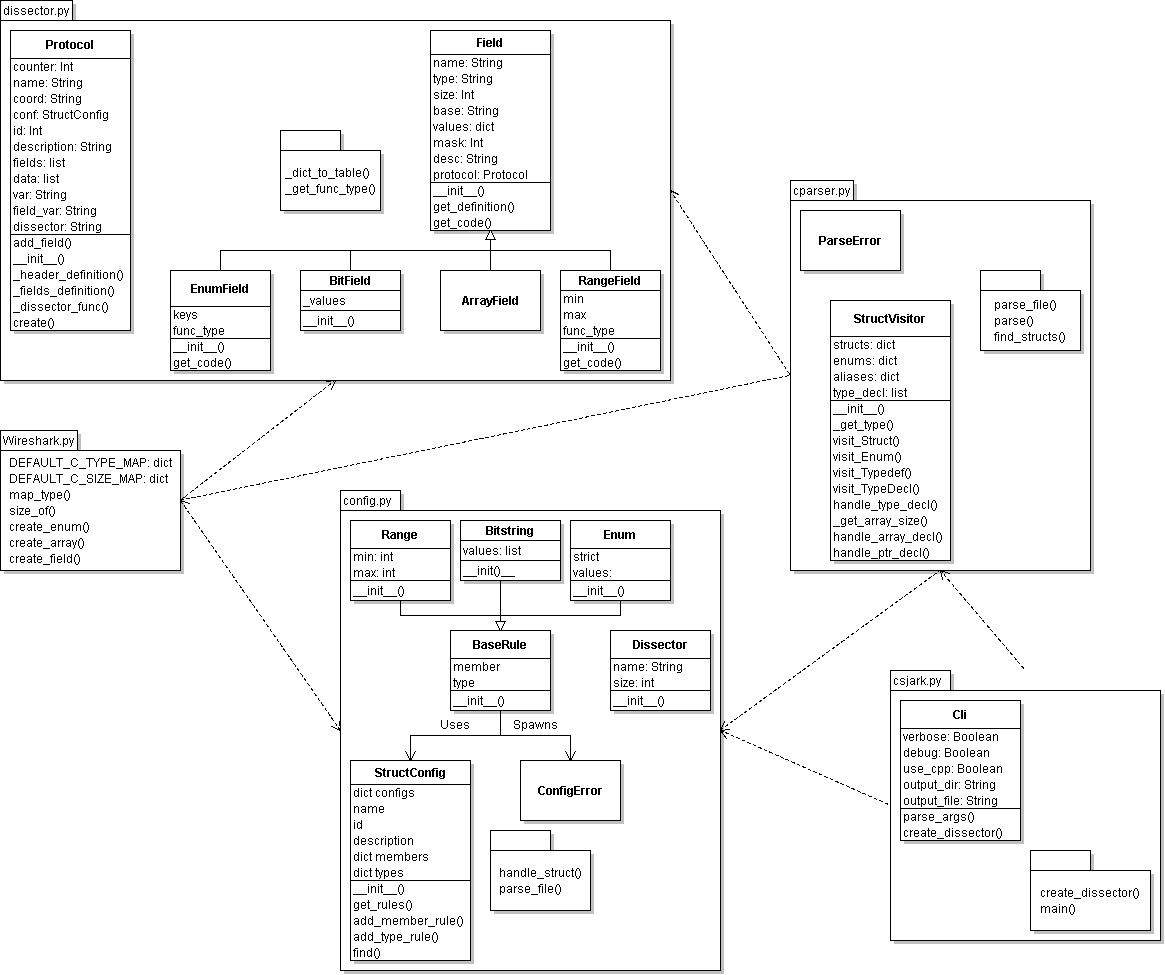
\includegraphics[width=\textwidth]{./sprints/img/class_diagram_s2}
	\caption{Class Diagram\label{fig:sp2:class}}
\end{figure}

%----------------------
\section{Implementation}
%----------------------

In the previous sprint we focused on creating a naive implementation of the 
utility. In this sprint the focus was on implementing data types for the 
C programming language and making it possible to configure more options on how 
the dissector will function. This section will cover the requirements 
implemented, how they were implemented and what the ''output'' looks like.

\subsection{Support Members of Type enum}
%----------------------
\label{sec:supportenum}
Enum is a type declaration in C, which specifies enumeration constants.  Enum 
is supported because it is a basic datatype in the C language. 
\autoref{code:cenum} shows an example of an enum in a C-header file. The 
Wireshark dissector will display the named value, making it 
easier to read, an example is shown in \autoref{fig:wscenum}. The red 
rectangle shows the enumerated named value.

\begin{figure}[ht]
	\center
	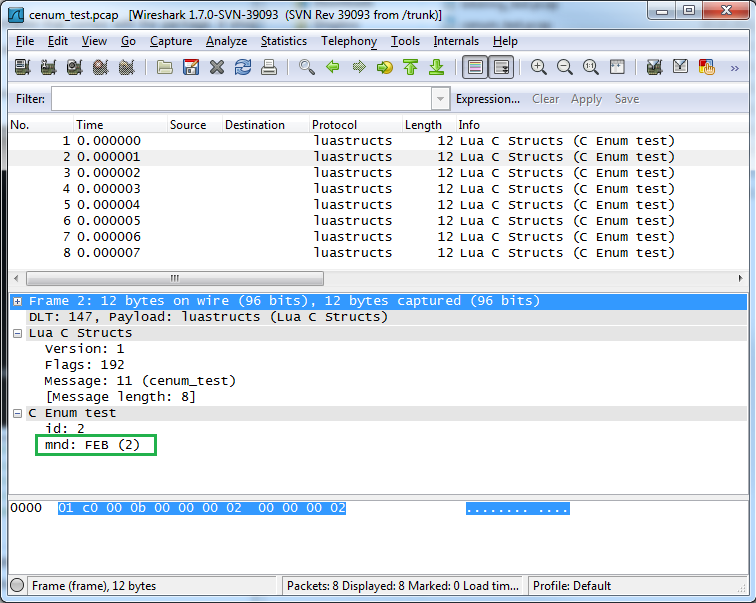
\includegraphics[width=\textwidth]{./sprints/img/wireshark_cenum}
	\caption{Enumeration in Wireshark\label{fig:wscenum}}
\end{figure}

\lstset{language=C,caption={Enum support},label=code:cenum}
\lstinputlisting[language=C]{./sprints/code/cenum_test.h}

\subsection{Support Members of Type Struct}
%----------------------
Structs are an important part of the C language, a struct declaration consists 
of a group of different fields, these fields can have any type, also struct. 
This was therefore an important requirement to implement. An example is shown 
in \autoref{code:structmember}.

\lstset{language=C,caption={Struct support},label=code:structmember}
\lstinputlisting[language=C]{./sprints/code/struct_member.h}

\subsection{Detect Structs with Same Name}
%----------------------
Two structs can have the same name, and therefore we needed a way of detecting it. 
If the parser finds two structs with the same name, an exception is 
raised, and the generation of the dissector is terminated.

\subsection{Support display of structs within structs}
%----------------------
The utility is able to display structs within a struct in Wireshark, the 
member will be visible, and the struct will be in a subtree that can be 
expanded. \autoref{fig:wsstructstruct} is a screenshot of this dissector in 
Wireshark.

\begin{figure}[ht]
	\center
	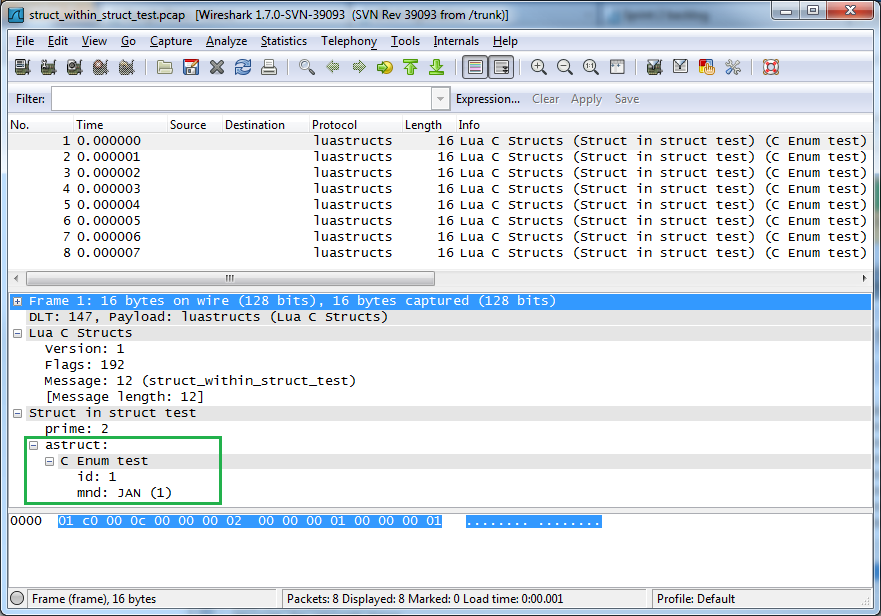
\includegraphics[width=\textwidth]{./sprints/img/wireshark_structwithstruct}
	\caption{Structs in Wireshark\label{fig:wsstructstruct}}
\end{figure}

\subsection{Support Enumerated Named Values}
%----------------------
In C there are two ways to do enumerations, the first option was explained in 
\autoref{sec:supportenum}, the other way is to use \#define which is shown in 
\autoref{code:defenum}. The advantage of using \#define is that the values 
can be generated. Since this cannot be understood by the parser, it can be 
generated directly from the header file, so it have to be supported by 
configuration. \autoref{code:enumconf}. The Lua-dissector will display the 
enum in the same way as in \autoref{sec:supportenum}.

\lstset{language=C,caption={Enumerated named values},label=code:defenum}
\lstinputlisting[language=C]{./sprints/code/def_enum.h}

\lstset{language=C,caption={Enumerated named values config},label=code:enumconf}
\lstinputlisting[language=C]{./sprints/code/def_enum.yml}

\subsection{Support for Bit Strings}
%----------------------
All bits in a basic data type can represent different values. An integer is 
represented by 4 bytes(32 bits), each of these bits can for example represent 
32 ''true/false' values. Our utility support configuration of these bits. Bits 
can be in groups, so they can represent more than two values. 
\autoref{code:bitstring} shows how bit string can be configured. 
\autoref{fig:wsbitstring} shows an example of how bit strings are displayed in 
Wireshark. Each group of bits are masked, so it is easier to see the values. 
The values are also named, if they are configured.

\begin{figure}[ht]
	\center
	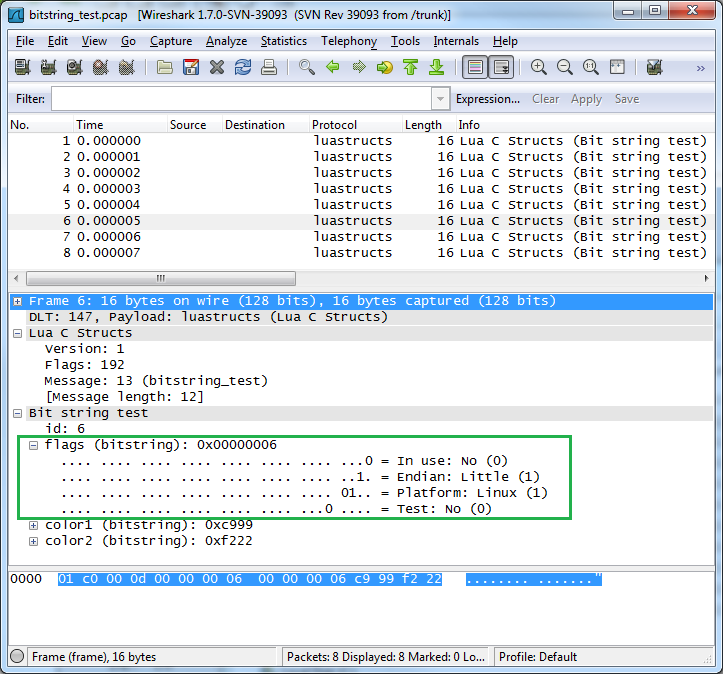
\includegraphics[width=\textwidth]{./sprints/img/wireshark_bitstring}
	\caption{Bit string in Wireshark\label{fig:wsbitstring}}
\end{figure}

\lstset{language=C,caption={Bitstring configuration},label=code:bitstring}
\lstinputlisting[language=C]{./sprints/code/bitstring.yml}

\subsection{Support Members of Type Array}
%----------------------
Csjark supports header-files with arrays, and is able to display them in 
Wireshark with the Lua-dissector. Csjark supports arrays of all data types 
implemented so far. The Wireshark dissector can display multidimensional 
arrays, and will create a new subtree for each dimension.  A representation of 
arrays in wireshark is displayed in \autoref{fig:wsarray}.

\begin{figure}[ht]
	\center
	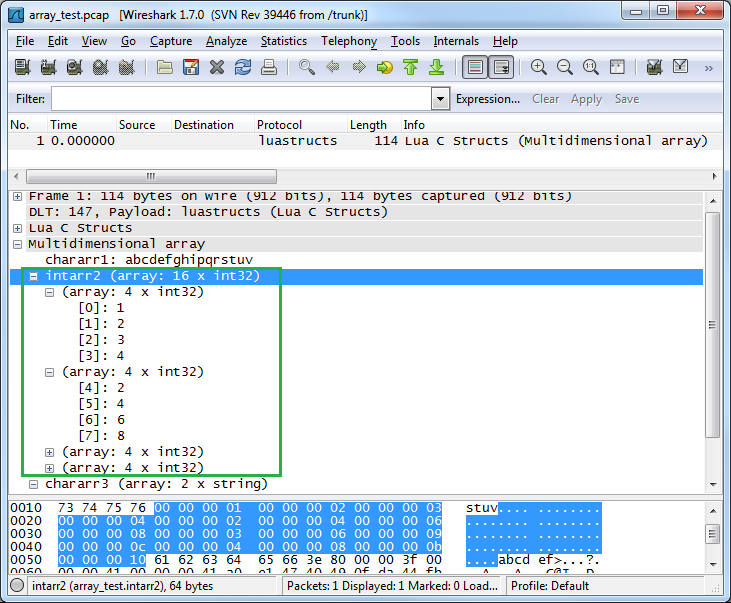
\includegraphics[width=\textwidth]{./sprints/img/wireshark_array}
	\caption{Arrays in Wireshark\label{fig:wsarray}}
\end{figure}

\subsection{Struct with Various Trailers}
%----------------------
The utility is able to support all kinds of trailers, that wireshark has 
built-in dissector for. Trailers are data that follows a struct, this can be 
any kind of data, but only trails that have built-in support in wireshark can 
be displayed.  To be able to use the wireshark dissectors, they have to be 
configured. In the example below, the wireshark dissector for ASN.1 
BER\footnote{Basic Encoding Rules}  is used.  In \autoref{code:trailer}, we 
specify ''asn1\_count'' as a member in the struct, this is used to tell the 
number of ASN.1 fields. The config in  \autoref{code:trailerconf} specifies 
fields with size of six bytest, the number of fields are specified by the data 
sent with the struct. At the end there is aa field of size five bytes. An 
example of ASN.1 in wireshark, can be seen in \autoref{fig:wstrailer}.

\begin{figure}[ht]
	\center
	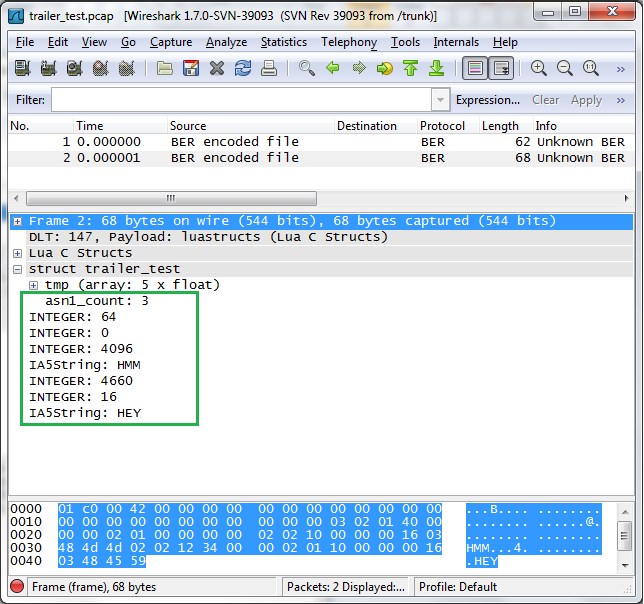
\includegraphics[width=\textwidth]{./sprints/img/wireshark_trailer}
	\caption{BER Trailer in Wireshark\label{fig:wstrailer}}
\end{figure}

\lstset{language=C,caption={Enumerated named values},label=code:trailer}
\lstinputlisting[language=C]{./sprints/code/trailer.h}

\lstset{language=C,caption={Enumerated named values config},label=code:trailerconf}
\lstinputlisting[language=C]{./sprints/code/trailer.yml}

\subsection{Custom Lua Configuration}
%----------------------
Csjark can support custom Lua configuration, by including Lua-scripts from a 
file specified in the configuration file. The reason for supporting custom Lua 
configuration is for protocols that are not built-in dissectors in Wireshark, 
and are not structs. The only way to support this, is to write a own dissector 
in Lua, and include it in the configuration. 
TODO: Not finished(add example + screenshot)

\subsection{Dissector ID}
%----------------------
All struct-packets that Wireshark captures, has a header, one of the fields in 
the header is the message id. This id is used to load the the correct 
dissector when a packet is captured. Each dissector should have a unique id, 
to avoid possible conflicts. This functionallity is implemented and the 
message id must be specified in the configuration file, \autoref{code:msgid} 
is an example of how this is done.

\lstset{language=C,caption={Dissector ID config},label=code:msgid}
\lstinputlisting[language=C]{./sprints/code/messageid.yml}

\subsection{Endian Handling}
%----------------------
Endian handling is postponed to the next sprint, because it is a platform 
specific problem, and should be implemented together with platform support.

\subsection{Folder Support in the CLI}
%----------------------
Folder support in the CLI\footnote{Command-line Interface} has been 
implemented, so it is possible to generate Lua-scripts for all structs stored 
in a given folder. At the moment, all dissectors will be regenerated. 
Functionality to only generate modified or new header-files will be added in 
the next sprint. \autoref{fig:csjarkfolder} is an example usage of CSjark where
the command first shows the usage of CSjark, and the second command 
generates dissectors from the folder ''header/'' and configurations from ''etc/''.

\begin{figure}[ht]
	\center
	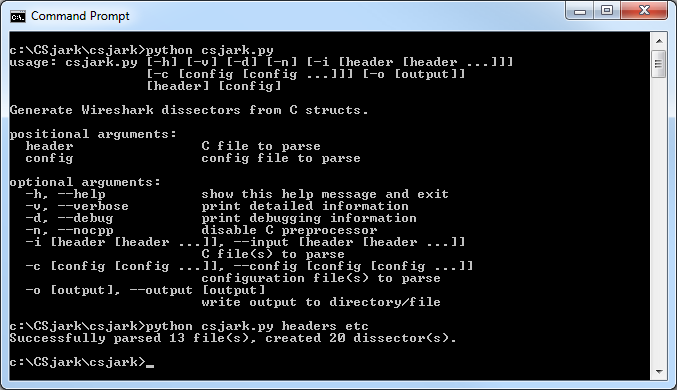
\includegraphics[width=\textwidth]{./sprints/img/csjark_folder}
	\caption{Arrays in Wireshark\label{fig:csjarkfolder}}
\end{figure}

\subsection{Support Custom Handling of Specified Data Types}
%----------------------
The utility supports custom handling of specific data types, this includes 
functionality to support  time\_t and nstime\_t. All basic data types and 
struct members can be configured to be handled in a special way. 
\autoref{code:customstruct} show an example of a struct with four members, two 
of them are time fields, and the last two is a BOOL and an integer to be 
handled in a custom way. This struct is configured in 
\autoref{code:customconfig}, in the config the two time fields are configured 
to be respectively absolute time and relative time, and the BOOL type to have 
a size of four bytes. The struct member ''all' is configured with an enumerated 
value, and will be visible as a hex-value. \autoref{fig:customdatatype} is a 
screenshot of the struct in Wireshark.

\begin{figure}[ht]
	\center
	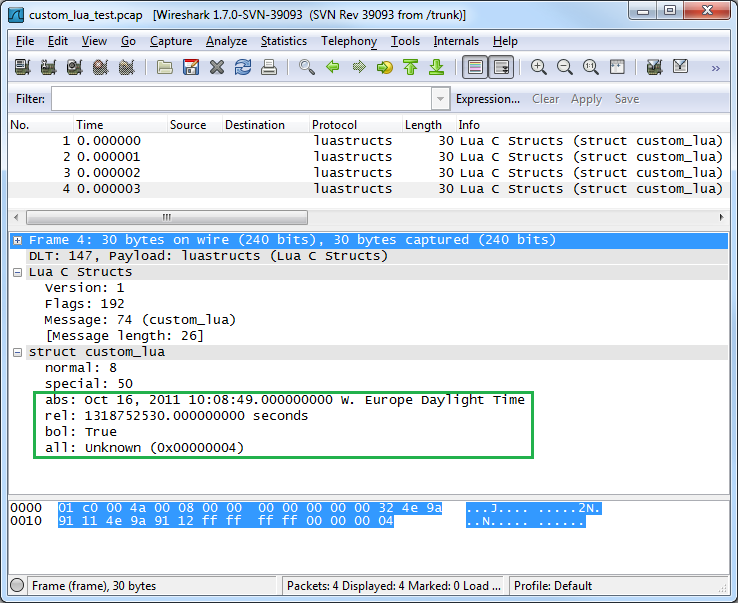
\includegraphics[width=\textwidth]{./sprints/img/wireshark_custom}
	\caption{Custom handling of Data Typesk\label{fig:customdatatype}}
\end{figure}

\lstset{language=C,caption={Struct for custom handling},label=code:customstruct}
\lstinputlisting[language=C]{./sprints/code/customfield.h}

\lstset{language=C,caption={Config for custom handling},label=code:customconfig}
\lstinputlisting[language=C]{./sprints/code/customfield.yml}

\subsection{Typedef Support}
%----------------------
Csjark is supporting the keyword typedef, which is a facility to create new 
data types names. \autoref{code:typedef} shows examples of typedef's that 
csjark supports.

\lstset{language=C,caption={Typedef example},label=code:typedef}
\lstinputlisting[language=C]{./sprints/code/typedef.h}

%-----------------------
\section{Sprint Testing}
%-----------------------
This section introduces the tests preformed during the sprint and their results. For sprint 2 it was also decided that the larger unit tests should also be documented and added to the test documents.

%subsection{Tests}
During the sprint the team executed a total of 6 tests with names as seen below. Tests executed:
\begin{itemize}
	\item TID08 - Supporting members of type enum \autoref{tab:sp2TID08}
	\item TID09 - Supporting members of type array  \autoref{tab:sp2TID09}
	\item TID10 - Supporting the display of structs within structs  \autoref{tab:sp2TID10}
	\item TID11 - Supporting enumerated named values  \autoref{tab:sp2TID11}
	\item TID12 - Supporting bit strings  \autoref{tab:sp2TID12}
	\item TID13 - Supporting structs with various trailers \autoref{tab:sp2TID13}
	\item TID14 - Sprint 2 functionality test \autoref{tab:sp2TID14}
\end{itemize}

\subsection{Test Results}
%----------------------------
\begin{table}[!htb] \footnotesize \center
\caption{Recognizing Supporting enums \label{tab:sp2TID08}}
\begin{tabular}{l l}
	\toprule
	Header & Description \\
	\midrule
	Description &  Supporting members of type enum  \\
	Tester & Lars Solvoll Tønder \\
	Date & 15.10.2011 \\
	Result & Success\\
	\bottomrule
\end{tabular}
\end{table}

\begin{table}[!htb] \footnotesize \center
\caption{Recognizing Supporting arrays \label{tab:sp2TID09}}
\begin{tabular}{l l}
	\toprule
	Header & Description \\
	\midrule
	Description &  Supporting members of type array   \\
	Tester & Lars Solvoll Tønder \\
	Date & 15.10.2011 \\
	Result & Success\\
	\bottomrule
\end{tabular}
\end{table}

\begin{table}[!htb] \footnotesize \center
\caption{Supporting the display of sctructs within structs \label{tab:sp2TID10}}
\begin{tabular}{l l}
	\toprule
	Header & Description \\
	\midrule
	Description &  Supporting the display of sctructs within structs \\
	Tester & Erik Bergersen \\
	Date & 17.10.2011 \\
	Result & Success. \\
	\bottomrule
\end{tabular}
\end{table}

\begin{table}[!htb] \footnotesize \center
\caption{Supporting enumerated name values \label{tab:sp2TID11}}
\begin{tabular}{l l}
	\toprule
	Header & Description \\
	\midrule
	Description &  Supporting enumerated name values \\
	Tester & Lars Solvoll Tønder \\
	Date & 17.10.2011 \\
	Result & Success\\
	\bottomrule
\end{tabular}
\end{table}


\begin{table}[!htb] \footnotesize \center
\caption{ Supporting bit strings \label{tab:sp2TID12}}
\begin{tabular}{l l}
	\toprule
	Header & Description \\
	\midrule
	Description & Supporting bit strings \\
	Tester & Lars Solvoll Tønder \\
	Date & 17.10.2011 \\
	Result & Success\\
	\bottomrule
\end{tabular}
\end{table}

\begin{table}[!htb] \footnotesize \center
\caption{Supporting structs with various trailers \label{tab:sp2TID13}}
\begin{tabular}{l l}
	\toprule
	Header & Description \\
	\midrule
	Description & Supporting structs with various trailers \\
	Tester & Erik Bergersen \\
	Date & 18.10.2011 \\
	Result & Success\\
	\bottomrule
\end{tabular}
\end{table}

\begin{table}[!htb] \footnotesize \center
\caption{Sprint 2 functionality test\label{tab:sp2TID14}}
\begin{tabular}{l l}
	\toprule
	Header & Description \\
	\midrule
	Description & unit test covering all of the functionality implemented in sprint 2 \\
	Tester & Lars Solvoll Tønder \\
	Date & 18.10.2011 \\
	Result & Success\\
	\bottomrule
\end{tabular}
\end{table}

\subsection{Test Evaluation}
%-------------------------------
For the second sprint the developers focused a lot more on testing during implementation. The team also decided that the testers should check how much of the code was covered in the unit tests. This made the group focus more on making proper unit tests that tests as much functionality as possible This had a very positive effect on the tests ran at the end of the sprint where not a single test failed, except for one test which ended up exposing a bug in Wireshark

\subsubsection{Test Coverage}
This section introduces the amount of code covered by our unit tests and how it relates to the test coverage from the previous sprints.
 MAKE A GRAPH OF THE CODE COVERAGE AND PUT IT HERE

 


%--------------------------
\section{Customer Feedback}
%--------------------------
\subsection{Requirement changes and feedback}
In sprint 2 we were able to demonstrate many of the requirements for the customer, and as a result we got some feedback of some changes and refinements that the customer wants. The customer also added some new features they would like to have. The changes and additions are listed bellow.

\subsubsection{FR1-E: Support members of type array}
Arrays should be displayed as a sublevel. Multidimensional arrays should have one sublevel per dimension. The dissector should also display the type of the array and show the different indexes for the sublevels.

\subsubsection{FR2-B: struct within structs}
The customer stated that the inner struct should be displayed as a sublevel of the outer struct.
When an external dissector is called, it should be called with name, and not id, so that structs that is never used as a base does not need to be assigned an id.

\subsubsection{FR4-C Custom handling of specific types}
The customer stated that they would like certain types to be interpreted in a certain way as default behaviour, but that the user should be able to configure specific behaviour for a specific member of a struct.

\subsubsection{FR4-E: Headers/trailers}
The customer originally stated that this feature included both headers and trailer structs for a given struct. This is now refined to mean that the given struct is the header, and that it can have various trailers (could be one or more c structs, ASN.1, etc.). A configuration file should specify the kind of trailer, and what variable inside the header struct which specify how many trailer items to expect. If the header does not specify the length of the trailer the dissector should just use the rest of the buffer, or the dissector is responsible to return the length used from the buffer, so the caller can give the rest to the next dissector.
In Wireshark it should be displayed as a sequence of structs.

\subsubsection{FR4-F: Support for integers that represents enumerated values and bit strings}
The customer clarified this by explaining that they wanted integers that represents an enumerated value to be displayed like an enum (member name and the string that represents the integer value) and that the bit strings should be displayed as a list with the name and value (1 / 0 or yes / no) of the different bits in the integer. It should also display the original integer I hex. As a result of this, the requirement was split into two:
\begin{itemize}
\item FR4-F	Support enumerated named values
\item FR4-G	Support for bit strings
\end{itemize}
The customer also confirmed that the bit strings are endian specific and that he would like then to start counting from 1 (not zero, as in our first implementation).

\subsubsection{FR5-C Endian handling}
The customer stated that the header part of the packed, which include the platform flag, will always be in big endian (network order).

\subsubsection{FR7-C: Batch mode}
The customer clarified this to mean that the utility should be able to run completely unattended given a set of command line arguments. For example it should not ask the users any questions under this modus. This is to be able to run it as a cron job at night.

\subsubsection{NR4: A user without prior knowledge should be able to use the tool within X hours.}
The customer defined X as 5.

\subsubsection{NR5: A user with prior knowledge should be able to use the tool within Y hours.}
The customer defined Y as 1.

\subsubsection{Detecting ambiguous struct definitions (more than one struct definition with the same name)}
The utility should detect if there are more that one struct with the same name. If found, the utility should exit with a proper error message because 

\subsubsection{Data alignment}
The customer said that we could have some problems with alignment with the current offsets, because the different platforms may pad the data members of a struct to match an integer number of words on that platform.

\subsubsection{Testability}
The customer suggested that we might want to refine some of the requirement to make them more testable. This can be done by adding more measurable goals.

\subsubsection{Documentation}
The documentation should specify what parameters are needed, like what parameters that should be passed to a dissector.

\subsubsection{Locating “missing” header files}
Some of the header files specified in a file might be located in an unknown location. The customer suggested that we should include a way to configure header location.

\subsubsection{What headers should the utility be generate dissectors for}
The customer suggested that we include a way to specify the relevant header files in a configuration file.

\subsubsection{Dissector id}
Only structs explicitly configured with an id should be assigned an id. The rest should be called by their textual name. This is to avoid id collisions and limit configuration needed.

\subsubsection{Headers and configuration the utility cannot handle}
The customer stated that they wanted the tool to continue generating dissectors even if it encounters a file it cannot handle. The tool should just give an appropriate error message and carry on with the next file.

\subsection{Customers feedback on the product}
The customer is satisfied with the progress of the utility and is so far pleased with its functionality. They also feel that the team are flexible when it comes to feature refinement and additions. 

%--------------------------
\section{Sprint Evaluation}
%--------------------------
This section contains the team evaluation of the second sprint.

\subsection{Review}
%--------------------------
The first sprint evaluation resulted in some planned actions for the forthcoming sprints. Looking back at these at this sprint evaluation, we quickly realized that we fell into the same pitfalls again: lack of documentation, bad work distribution and reverse engineering of vital parts.

The sprint started out very good. We had a four-hour long planning meeting, and ended up with a good backlog and a common understanding of the technical aspects of the sprint. Even though the meeting was significantly better this time, we failed in doing the design early. User stories was postponed till the middle of the sprint and they were written by team members that had no understanding of the code. Doing them in a reverse engineered fashion ended up being more work than expected. This is something that we definitely have to change, if we want to do Scrum properly. We have decided that at the next planning meeting, we will use as many hours as it takes to end up with a good plan, documentation and user stories.

The rest of the sprint was as expected. Implementation went smoothly and the customer are satisified of our progress. The documentation of progress was not good. We write most of the parts that the advisers want to look at, but we do not gather all information in one document. We have done that at the end of the sprint. 



\subsection{Positive Experiences}
%--------------------------
\begin{itemize}
	\item A significantly better sprint planning meeting
	\item All the team members have raised their effort, working more hours
	\item Accurate time estimates
	\item Successful presentation of the utility to the customer
	\begin {itemize}
		\item Implementation of features work as intended
		\item Good feedback from the customer
	\end{itemize}
	\item Thriving team atmosphere
\end{itemize}



\subsection{Negative Experiences}
%--------------------------
\begin{itemize}
	\item The planning meeting was too short, which resulted in a shortcomming in the documentation.
	\item Documentation was postponed till the end again
	\item Lack of feedback to the advisor
	\item Bad work balance
	\item Could not complete all the tasks in the backlog
\end{itemize}


\subsection{Planned Actions}
%--------------------------


\subsection{Barriers}
%--------------------------
\subsubsection{The work distrubution} 
As mentioned in the review, the team had a uneven work distribution. Some team members were eager to start implementing and took all the implementation tasks, leaving mostly documentation tasks for the rest of the team. The documentation tasks are closely connected to the implementation, so this resulted in problems. Documentation were postponed till the end.

The planned actions section describes how we are planning to avoid that this happens again. 

\subsubsection{Wireshark} 
































%=================
\chapter{Sprint 3}
%=================


%------------------------
\section{Sprint Planning}
%------------------------
For the third sprint we intend to implement the remanding requirements in the product backlog. We feel that the first and second sprint has resulted in a satisfying \gls{utility}, but it is still missing important functionality.

After two sprint iterations, we are still trying to improve our approach to \Gls{scrum}. Each sprint results in new ideas and better ways to do the process, and in this sprint we want everything to be correct and in the right order.\\
\\
There will be two major changes this sprint:
\begin {itemize}
\item We will have a complete planning meeting. The meeting should result in a good planning document, user stories for all the requirements, complete set of work items in the sprint backlog and a early understanding of the design. This approach will be differently from earlier sprints, where user stories was written in parallel with implementation. The user story should now be in place before the implementation, and the implementation should be based on the user story. This will make documenting the process easier, and will in turn give the advisors more documentation of what we are doing. Then we can receive valuable feedback from them.

\item In the sprint backlog we will have work items for every task that needs to be done throughout the sprint, including writing minutes, doing documentation, implementation and so on.  Assignment of responsibilities for items in the backlog should not be done at the planning meeting, we rather only give responsibility for one item for each team member at a time. The rest of the items will be unassigned. At each stand-up meeting we pick a task and must be done before the next meeting. This will ensure efficiency and the work done by others are easier to check and revise. It will give us a better work balance, as no team member can gap over too many tasks and leave none for the others.
\end{itemize}
We think that these changes will improve our work efficiency, and make sprint 3 the best one so far.


\subsection{Duration}
%-----------------------

The sprint started with the planning meeting the 19th of October and our work started the following day. The sprint duration is 14 days, and will end the 1st of November with a review meeting. 


\subsection{Sprint Goal}
%-----------------------
For the third sprint the team will update CSjark to version 0.3 which will extend the \gls{utility} so that it contains the complete functionality requested by the customer at this phase of the project. In this sprint we will pick all of the current requirements from the product backlog as all of the underlying functionality needed for them are already in place from the previous sprints. This means that we will also aim to create a draft of the final design of the system during the sprint.

The most important function that is going to be implemented in this sprint is being able to display packets from different originating platforms properly. This will be implemented by having every \gls{packet} contain a flag specifying their originating platform, and by having our \glspl{dissector} use this flag value to influence how it handles the data in the \gls{packet}.

\subsection{Back Log}
%--------------------
The work items concering features for this sprint are listed in Table \ref{tab:sprint3req}. These are covered by user stories and are about a fourth of the work in this sprint. See the timetable for the other work items.\\
Timetable for this sprint: Table \ref{tab:sprint3time}.\\

\begin{table}[!htb] \small \center
\caption{Sprint 3 Requirement Work Items \label{tab:sprint3req}}
\begin{tabularx}{\textwidth}{l X c c}
	\toprule
	& & \multicolumn{2}{c}{Hours} \\
	\cmidrule(r){3-4}
	User story & Req. and Description & Est. & Act. \\
	\midrule
	\textbf{Impl.} &  & \textbf{56} & \textbf{-} \\
	\hyperref[tab:req:stories7]{US29} & FR5-A: Flags specified for each platform &  5  & - \\
	\hyperref[tab:req:stories8]{US31} & FR5-C: \Gls{dissector} support both little and big \gls{endian} & 5  & - \\
	\hyperref[tab:req:stories8]{US32} & FR5-D: \Gls{dissector} support different sizes from flags & 12  & - \\
	\hyperref[tab:req:stories8]{US33} & FR3-C: Support WIN32, WIN64,\GLS{sparc} etc &  5  & - \\
	\hyperref[tab:req:stories7]{US29} & FR4-B: Configuration supports custom \Gls{lua} files & 6 & -\\
	\hyperref[tab:req:stories7]{US28} & FR2-C: Support \Gls{wireshark} filter and search on attributes &  3 & -\\
	\hyperref[tab:req:stories7]{US29} & FR5-B: \Glspl{dissector} support memory alignement & 4 & -\\
	\hyperref[tab:req:stories7]{US26} & FR1-D: Support members of type \gls{union} & 5  & -\\
	\hyperref[tab:req:stories7]{US27} & FR2-A add: Display a wildcard type for valid c types that \Gls{wireshark} has no support for & 3  & - \\
	\hyperref[tab:req:stories9]{US35} & FR4-D mod: Support specifying the ID of \glspl{dissector} (name and function) & 3  & - \\
	\hyperref[tab:req:stories9]{US39} & FR6-D: Don’t regenerate \glspl{dissector} & 1 & - \\
	\hyperref[tab:req:stories7]{US29} & FR2: Handle \Gls{lua} reserved definition names & 2 & - \\
	\addlinespace
	\textbf{Testing} &  & \textbf{19} & \textbf{-} \\
	 & FR4-B: Custom \Gls{lua} configuration & 2 & - \\
	 & FR5-C: \Glspl{dissector} support both little and big \gls{endian} & 1 & - \\
	 & FR5-D: \Glspl{dissector} support different sizes from flags & 2 & - \\
	 & FR3-C: Support WIN32, WIN64, \GLS{sparc} etc & 4 & - \\
	 & FR5-B: \Glspl{dissector} support memory alignement & 8 & - \\
	 & FR1-D: Support members of type \gls{union} & 1 & - \\
	 & FR2: Handle \Gls{lua} reserved definition names & 1 & - \\
	\addlinespace
	\textbf{Doc.} &  & \textbf{11} & \textbf{-} \\
	 & FR4-B: Custom \Gls{lua} configuration & 2 & - \\
	\hyperref[tab:req:stories8]{US34} & FR4-C: Support custom handling of specific data types & 2 & - \\
	\hyperref[tab:req:stories9]{US36} & FR5: User documentation for what platform that the \gls{utility} support & 3 & - \\
	\hyperref[tab:req:stories9]{US37} & FR5: Create developer manual from python docstrings (autodoc plugin) & 4 & - \\
	\addlinespace
	\textbf{Fixes} &  & \textbf{16} & \textbf{-} \\
	\midrule
	& Total: & 102 &  -\\
	\bottomrule
\end{tabularx}
\end{table}


\begin{table}[!htb] \small \center
\caption{Sprint 3 Timetable\label{tab:sprint3time}}
\begin{tabularx}{\textwidth}{X c c}
	\toprule
	& \multicolumn{2}{c}{Hours} \\
	\cmidrule(r){2-3}
	Description & Est. & Act. \\
	\midrule
	\textbf{Sprint planning} & \textbf{30} & \textbf{47.5} \\
	\addlinespace
	\textbf{Sprint 3 requirements} & \textbf{102} & \textbf{-} \\
	Implementation & 56 & - \\
	Testing & 19 & - \\
	User Documentation & 11 & - \\
	Fixes & 16 & - \\
	\addlinespace
	\textbf{Sprint review} & \textbf{20} & \textbf{-} \\
	\addlinespace
	\textbf{Sprint documentation} & \textbf{75} & \textbf{-} \\
	Sprint 1 document & 10 & -\\
	Sprint 2 document & 14 & - \\
	Sprint 3 document & 51 & - \\
	\addlinespace
	\textbf{Report work} & \textbf{42} & \textbf{-} \\
	User stories to LaTeX & 3 & 4\\
	Architecture update & 8 & -\\
	Glossaries and acronyms & 16 & -\\
	Requirement review & 15 & -\\
	Layout and correction & 15 & -\\
	\addlinespace
	\textbf{Lectures} & \textbf{21} & \textbf{14} \\
	\addlinespace
	\textbf{Meetings} & \textbf{57} & \textbf{-} \\
	Advisor meetings & 28 & - \\
	Customer meetings & 8 & - \\
	Stand-up meetings & 21 & - \\
	\textbf{Project management} & \textbf{20} & \textbf{-} \\
	\midrule
	Total: & 367 & - \\
	\bottomrule
\end{tabularx}
\end{table}



%----------------------
\section{System Design}
%----------------------
The system design defines the new modules and architecture that has to be in place to satisfy the specified requirements that we have included in the sprint 3 backlog. Most of the design are already done in earlier sprints; now we extend that and add some new elements.

\subsection{System overview}
%----------------------
Now that the \gls{utility} has both basic and advanced features, it is time to specialize and make support for environmental variables that can be found in Thales' source code. This basically include various platform specific support, \gls{endian} handling and minor technicalities. The latter one is vital for the customer in order for the \gls{utility} to be efficient and adequate.

\subsubsection{Platform specific support}
We know that the various platforms behave differently, and this must be supported by our \gls{utility}. The customer has mentioned at least three platforms that we have to support. As we emphasize extensibility and modifiability, it must also be expected that new platforms will be added or removed to the supported platforms in the future. Thereby we will try to make the set-up for support easily understandable.

We have decided that the platform definition will be a subpart of a flag-field in the structs header. To ensure modifiability we will assign a 16 bit field for this, giving the developers possibility to have 65536 unique platforms. From this we imagine that the platform flag can point to a dictionary which has the following information about the actual platform:
\begin{itemize}
\item Endianness
\item Length of fields
\item Memory alignment
\end{itemize}
All these three fields must be combined to enable the utility to generate a \gls{dissector} that will dissect the struct correctly.\\

The use of this information will be done in the config module, as you can see in the new class diagram MAKE REF.

\subsubsection{Dicitonary lookup}
Deciding how to implement handling of different platforms ended in a design draft seen in Figure \autoref{fig:platformhandling}. The \gls{dissector} module will make a dictionary lookup in the table of supported platforms. This table conatins all platforms that the \gls{utility} can make \glspl{dissector} for, and their information of how the \gls{dissector} shall be encoded to achieve correct handling of \gls{endianness}, length of fields and memory alignment.
We will start out by hardcoding this into the source code, but in the end we want to have this feed to the \gls{utility} through a configuration-file. This is the way the customer has envisioned it.  

%\begin{figure}[!htb]
%	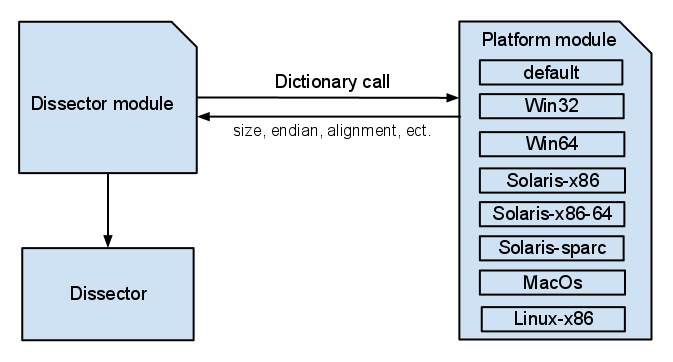
\includegraphics[width=\textwidth]{./sprints/img/platformhandling}
%	\caption{Platform handling\label{fig:platformhandling}}
%\end{figure}


\subsubsection{Endianness}
An important feature is the support for different endian handling. Endianness defines how the bits are ordered in the struct. It tells what bit is the most significant, and thereby the value that the bits represent. See the figure \ref{fig:endianness}.

\begin{figure}[!htb]
	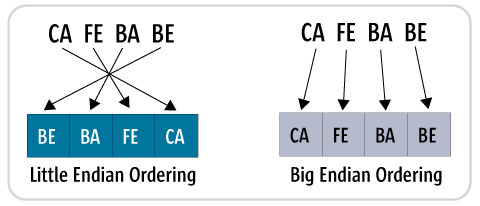
\includegraphics[width=\textwidth]{./sprints/img/endianness}
	\caption{Endianness\label{fig:endianness}}
\end{figure}

A design decision we made in the 
We know that Wireshark has support for reading both big- and little-endian. We understood that if the header could both be big and little endian, we would have problems, but Thales ensure us that headers always appear as small endian. So we need to dissect the data blob, which can be either big or small endian. By using the built-in reader support for endianness in Wireshark gave us much for free, but 


\subsubsection{Filter and search in \Gls{wireshark}}
The amount of data that are collected and dissected can be very large. The need for a filter and search mechanism is apparent. \Gls{wireshark} has this built-in, and the customer want the \gls{utility} to support it. To do that, we need to pass the abbrevation fields to Wireshark. These abbrevations will be generated by the dissector module and stored in the dissector made by the utility. Wireshark collects these when the actual dissector is used, and then a user will be able to search for them. In the design we have emphesized and assured us that the chosen abbrevations are descriptive, as the customer has stated it important in earlier customer meetings. 

\subsubsection{Technicalities}
Our design, and thereby implementation, will be influenced by Stig. He is a core developer for Wireshark and professional Python programmer. He points out things that we have done earlier that might not be efficient or not correct use. We have got some feedback on how elements should be passed to Wireshark.


\subsubsection{Batch processing}
The batch processing was implemented in the second sprint, but we need to modifiy it to make it able to process header-files even though it encounter some that it can not make dissectors for. 

%-----------------------
\section{Implementation}
%-----------------------
The main focus for this sprint was to support of different platforms. Several 
things are dependent on platform; \gls{endianness}, the memory allingment and sizes 
of data types. It is also possible that structs can be defined differnt for 
each platform. The \gls{utility} will generate different \glspl{dissector} for each 
platform. A \gls{dissector} this wil detect the platform and use the correct 
platform \gls{dissector}.

Support for the \gls{union} data type, finishing implementation of custom \Gls{lua} files 
and modification of functionallity implemented in the previous sprint was also 
done in this sprint.

\subsection{Specify Flags for Each Platform}
%-----------------------
It is necessary to specify flags for each platform to make it possible to 
correctly detect and display packages that wireshark captures. In wireshark 
the flags are used to tell which platform the \gls{packet} is sent from, so that 
the right \gls{dissector} is used to display the packets in \Gls{wireshark}. In the 
\gls{utility} the flag points to what kind of \gls{endianness}, how memory is aligned and 
the different sizes that is used for data types on the platform. These data 
are used to genereate a \gls{dissector} for the specific platform.

\subsection{Support Little and Big \Gls{endian}}
%-----------------------
Different platforms can order bytes in either little(left-to-right) or 
big(right-to-left) \gls{endian}. The \Gls{Windows} platform uses little \gls{endian}, and \GLS{sparc} 
uses big \gls{endian}. Since the \gls{utility} has to support both platforms, it was 
necessary to support handling of \gls{endianness}. The \Gls{lua} API in wireshark has 
functionallity to display data in both little and big \gls{endian}. Therefore the 
\gls{utility} has to read the specfied flag for the platform, and generate a \Gls{lua} 
\gls{dissector} that displays the data correctly for the given platform.

\subsection{Support Different Sizes from Flags}
%-----------------------
On different platforms, there can be different sizes on the data types. For 
example on windows a \emph{long double} is 8 bytes, and on sparc it is 16 
bytes. It is possible to specify sizes for data types for each platform. All 
these specifications is written in python code, and are easy to modify for the 
user of the system.

\subsection{Support Platform Specific Macros}
%-----------------------
All c complilers have predefined macros for different operating systems and 
processors. These macros are much used in code that need to be portabel for 
different platforms. When using these macros it is possible to create 
different struct members for each operating system, as shown in 
\autoref{code:predefmacro}, which will use different data types on each 
operating system. All platform specific macros are specified for each 
platform, so the dissector is generated correctly for each of the platforms. 
Currently all the platform specifications is done in python code.

\lstset{language=C,caption={Macros in C},label=code:predefmacro}
\lstinputlisting[language=C]{./sprints/code/predefmacro.h}

\subsection{Support Custom \Gls{lua} Files}
%-----------------------
Implementation of this feature started in sprint 2, and support for using 
conformance file to add lua code to correct places in the lua dissector was 
finished in this sprint. With the conformance file it is possible to add code 
before and after an member in both the definition and function part of the 
dissector. It also possible to replace the code for a member in both of these 
sections. In the example below there is written custom lua for a 
struct(temperature) with on integer member(celsius). In the conformance file 
in \autoref{code:customcnf} there added three lines of comments as a custom 
Lua code, that are going to be added to the Lua dissector. In 
\autoref{code:customlua} it is possible to see the custom Lua code that was 
added to the Lua dissector. The first comment is added after the member 
definition. The two other comments are added above and below the member in the 
function part of the Lua dissector.

\lstset{language=C,caption={Custom Lua conformance file},label=code:customcnf}
\lstinputlisting[language=C]{./sprints/code/custom.cnf}

\lstset{language=C,caption={Custom Lua dissector code},label=code:customlua}
\lstinputlisting[language=C]{./sprints/code/custom.lua}

\subsection{Support \Gls{wireshark} Filter and Search}
%-----------------------
Wireshark has a display filter, where it is possible to use packet filtering. 
Each field in our genereated dissectors has a abbrevation name that is 
connected to a struct. For each member of a struct, it is possible to filter 
for a value. An example is shown in \autoref{fig:wsfilter}, this shows a 
filtering for packets where Trondheim is equal to the member \emph{place} in 
the struct \emph{postcode}. 

\begin{figure}[ht]
	\center
	\includegraphics[width=\textwidth]{./sprints/img/wireshark_filter}
	\caption{Union type support\label{fig:wsfilter}}
\end{figure}

\subsection{Support Different Memory Alignment}
%-----------------------
Since the dissectors generated by the utility, are going to be used for inter-process commuincation, it is important to handle memory alignment, because the packet that Wireshark capture is only a copy of the memory. Memory alignment is how the data are stored in the memory... 

An example?

TODO: Not finished

\subsection{Support Union Type}
%-----------------------
The \gls{union} type is a variabel that can contain different data types with 
different sizes. The \gls{union} will allocated memory for the largest type defined 
in the \gls{union}. \autoref{code:union} shows an example on a header-file with an 
\gls{union} type. The compiler is responisble for keeping track of size and 
alignment requirements\cite[p.147]{Kerninghan1988} . Since there is not 
possible to find out which data type that is used in \Gls{wireshark}, the \gls{utility} 
has to genereate a \gls{dissector} that display the values for each data type. 
\autoref{fig:wsunion} displays the \gls{dissector} generated from the struct in 
\autoref{code:union}, this shows the \gls{union} with three members, all of them are 
listed with their values, in this case the float value is the correct one.

\begin{figure}[ht]
	\center
	\includegraphics[width=\textwidth]{./sprints/img/wireshark_union}
	\caption{Union type support\label{fig:wsunion}}
\end{figure}

\lstset{language=C,caption={Union type},label=code:union}
\lstinputlisting[language=C]{./sprints/code/union.h}

\subsection{Display Types \Gls{wireshark} Do Not Support}
%-----------------------
The utility is able to genereate dissectors for C data types, that Wireshark 
do not support. When such a data type occour, Wireshark will display only 
display the packet data. An example of a data type, which Wireshark do not 
support is \emph{long double} on the sparc platform, which is a 128-bit foat. 
For this Wireshark will display the 16 bytes in hexadecimal.

\subsection{Support Specifying ID of \Glspl{dissector}}
%-----------------------
Specifying \gls{dissector} ID has been modified from sprint 2. The \gls{dissector} will 
still use the ID given in the configuration for a struct, if the struct is not 
given an ID in the configuration, then the ID for the struct will be set to 
\emph{NONE}. This is done to ensure that structs have an unique ID for their 
\gls{dissector}. Structs-in-structs member do not need an ID since they are called 
from the struct' by the \gls{dissector} name.

\subsection{Do Not Regenerate \glspl{dissector}}
%-----------------------
To increase the performance on generation of dissectors, dissectors that 
allready are genereated in batch mode, will only be generated once in a batch 
mode execution. This feature will be improved in the next sprint, so it only 
genereates dissectors in batch mode that are modified or new since the last 
batch run.

\subsection{Handle \Gls{lua} Reserved Keywords}
%-----------------------
\Gls{lua} has a list of reserved keywords, and some of these keywords are allowed in 
the C language. The \gls{utility} is able to support this under generation of \Gls{lua} 
code, when an identifier is a lua keyword, an underscore(\_) is added, so the 
identifier start with ''\_''.

\subsection{Support for Complex Arrays}
%-----------------------
Support for typedef was implemented in the previous sprint, in this sprint it 
has been improved to also support type definitions of complex arrays. Support 
for type definition of array is implemented, an example of such type 
definition in c is shown in \autoref{code:typedefarray}. Also support for 
arrays of enums, arrays, structs and pointers has been added.

\lstset{language=C,caption={Typedef of arrays},label=code:typedefarray}
\lstinputlisting[language=C]{./sprints/code/typedefarray.h}

%-----------------------
\section{Sprint Testing}
%-----------------------
During sprint 3 the team executed a total of 9 tests were run, but no additional testingfeatures were added during the sprint. Tests executed:

\begin{itemize}
	\item TID15 - Supporting batch mode of C header and configuration files \autoref{tab:sp3TID15}
	\item TID16 - Supporting custom \Gls{lua} configuration \autoref{tab:sp3TID16}
	\item TID17 - Supporting unions \autoref{tab:sp3TID17}
	\item TID18 - Supporting filter and search in wireshark \autoref{tab:sp3TID18}
	\item TID19 - Supporting WIN32, \_WIN64, \_SPARC etc \autoref{tab:sp3TID19}
	\item TID20 -  Supporting the use of flags specifying platforms to display member values correctly \autoref{tab:sp3TID20}
	\item TID21 - Supporting platforms with different \glspl{endian} \autoref{tab:sp3TID21}
	\item TID22 - Supporting alignments \autoref{tab:sp3TID22}
\end{itemize}

\begin{table}[!htb] \footnotesize \center
\caption{Supporting batch mode of C-headers and configuration files\label{tab:sp3TID15}}
\begin{tabular}{l l}
	\toprule
	Header & Description \\
	\midrule
	Description & Supporting batch mode of C header and configuration files \\
	Tester & Lars Solvoll Tønder \\
	Date & 28.10.2011 \\
	Result & Success\\
	\bottomrule
\end{tabular}
\end{table}

\begin{table}[!htb] \footnotesize \center
\caption{Supporting custom \Gls{lua} configuration\label{tab:sp3TID16}}
\begin{tabular}{l l}
	\toprule
	Header & Description \\
	\midrule
	Description & Supporting custom LUA configuration\\
	Tester & Lars Solvoll Tønder \\
	Date & 30.10.2011\\
	Result & success\\
	\bottomrule
\end{tabular}
\end{table}

\begin{table}[!htb] \footnotesize \center
\caption{Supporting unions\label{tab:sp3TID17}}
\begin{tabular}{l l}
	\toprule
	Header & Description \\
	\midrule
	Description & Supporting unions\\
	Tester & Lars Solvoll Tønder\\
	Date & 30.10.2011\\
	Result & success\\
	\bottomrule
\end{tabular}
\end{table}

\begin{table}[!htb] \footnotesize \center
\caption{Supporting filter and search in wireshark\label{tab:sp3TID18}}
\begin{tabular}{l l}
	\toprule
	Header & Description \\
	\midrule
	Description & Supporting filter and search in wireshark\\
	Tester & Lars Solvoll Tønder \\
	Date & 30.10.2011\\
	Result & success\\
	\bottomrule
\end{tabular}
\end{table}

\begin{table}[!htb] \footnotesize \center
\caption{Supporting WIN32, \_WIN64, \_\GLS{sparc} \label{tab:sp3TID19}}
\begin{tabular}{l l}
	\toprule
	Header & Description \\
	\midrule
	Description & Supporting WIN32, \_WIN64, \_\GLS{sparc} \\
	Tester & Lars Solvoll tønder\\
	Date & 30.10.2011\\
	Result & Failure. Most values were displayed correctly, but there were cases where the members and their values were different. Most notably in \gls{packet} 2 and 3 in the win64 and win32 \glspl{pcap-file} \\
	\bottomrule
\end{tabular}
\end{table}

\begin{table}[!htb] \footnotesize \center
\caption{Supporting the use of flags specifying platforms to display member values correctly \label{tab:sp3TID20}}
\begin{tabular}{l l}
	\toprule
	Header & Description \\
	\midrule
	Description & Supporting the use of flags specifying platforms to display member values correctly \\
	Tester & Lars Solvoll Tønder\\
	Date & 30.10.2011\\
	Result & Success\\
	\bottomrule
\end{tabular}
\end{table}

\begin{table}[!htb] \footnotesize \center
\caption{Supporting platforms with different \gls{endian} \label{tab:sp3TID21}}
\begin{tabular}{l l}
	\toprule
	Header & Description \\
	\midrule
	Description & Supporting platforms with different \gls{endian} \\
	Tester & Erik Bergersen\\
	Date & 31.10.2011\\
	Result & Success\\
	\bottomrule
\end{tabular}
\end{table}

\begin{table}[!htb] \footnotesize \center
\caption{Supporting alignments \label{tab:sp3TID22}}
\begin{tabular}{l l}
	\toprule
	Header & Description \\
	\midrule
	Description & Supporting alignments \\
	Tester & Lars Solvoll Tønder\\
	Date & 30.10.2011\\
	Result & Failure. All of the platforms that were used for testing were the same\\
	\bottomrule
\end{tabular}
\end{table}

\begin{table}[!htb] \footnotesize \center
\caption{Handling \Gls{lua} keywords \label{tab:sp3TID22}}
\begin{tabular}{l l}
	\toprule
	Header & Description \\
	\midrule
	Description & Handling \Gls{lua} keywords \\
	Tester & Lars Solvoll Tønder\\
	Date & 30.10.2011\\
	Result & Success\\
	\bottomrule
\end{tabular}
\end{table}

\subsection{Test Evaluation}

\subsubsection{Test Coverage}

%--------------------------
\section{Customer Feedback}
%--------------------------

\subsection{Pre-sprint}

The customer was satisfied with the functionality we implemented in sprint 2.
They feel that we are flexible and adapt well to their needs.
Some of the features from sprint 2 were postponed to sprint 3 because we needed additional feedback from the customer.
These include endianness and completing the handling of custom Lua files.

\subsubsection{New requirements}

We have assigned all the remaining requirements in the product backlog for this sprint.
If we are able to complete all the implementation tasks, the customer will provide us with more requirements for sprint 4.
The customer wants our utility to be as automatic as possible, and with as little configuration as possible. 
Additional requirements for sprint 4 will address optimization of the utility.

\subsection{During sprint}

In sprint 3 we again demonstrated our utility to the customer, and as a result we got some feedback on changes
and improvements we could make. The changes and additions are listed below.

\subsubsection{Wireshark, support of search and filter}

To support this the abbreviation field needs to be in place in our code

\subsubsection{Structs within structs}

The customer thought we displayed too much information in the info column in Wireshark,
 we should only display the name of the outer struct.

\subsubsection{Platforms}

We should not generate separate dissector files for the different platforms. It is much better if we have one protocol
with different functions for the different platforms, as this would not be such a performance hit.

\subsubsection{Flag values}

The customer said that our flag values were inconsistent, some flag values were platform names and some were operating
system names. They suggested using flags such as Solaris-x86, Solaris-SPARC, Win32 and Linux-x86.

\subsubsection{Testing of customer's header files}

The customer stressed the importance of our utility being able to run on the header files they have provided.
Once our utility is able to do this they can begin testing the utility on their own data.
We can expect to get a lot more feedback on the utility when they can test it themselves.


\subsection{The backlog and suggestions for sprint 4}

The customer was satisfied with the backlog for sprint 3.
They made several suggestions on features that could improve the utility, that we could implement in sprint 4.
These are listed below.

\subsubsection{Unitialized Memory}

It would be a nice if our utility were able to detect unitialized memory while debugging.
Different compilers use default patterns in members that are unitialized. If our utility could detect these patterns,
we could display the data in Wireshark with a warning that lets the user know that the data might have been unitialized.

\subsubsection{Dissector Ids}

The customer informed us that a struct could belong to several dissector IDs.
We should implement this by specifying a list of IDs instead of just a single one.

\subsubsection{Include dependency}

Christian describes that some structs may be included in other structs, which are resident in a different header file
not directly included in the  first, but both are included in a third header/source file. This creates a dependency which we must take
into consideration and implement in the utility.
TODO Rewrite this to english

\subsubsection{Specifying file name endings in batch mode}

The customer would like to be able to specify the file name endings of the files that are to be created dissectors for,
when running the utility in batch mode. The utility only needs to examine header files. The header files will have one or more known
file extensions, for example, .h and .hpp.

\subsubsection{Overall customer satisfaction}

In general the customer is satisfied with the progress we have made so far. Most of the requirements are
implemented or close to completion. When the utility is ready to be tested on their code, we can expect to receive
a lot of feedback on things we need to fix and improve.


















%--------------------------
\section{Sprint Evaluation}
%--------------------------



%=================
\chapter{Sprint 4}
%=================
This chapter contains the description of the work done in sprint 4. The 
chapter is diveded into sprint planning in \autoref{sec:sp4planning}, design 
done during the sprint in \autoref{sec:sp4design}, the implementation in 
\autoref{sec:sp4impl}, the result of the sprint testing in 
\autoref{sec:sp4test}, feedback the customer gave us during the sprint in 
\autoref{sec:sp4feedback} and evaluation of the sprint in 
\autoref{sec:sp4eval}.

%------------------------
\section{Sprint Planning}
%------------------------
\label{sec:sp4planning}
The fourth sprint will be the last iteration of this project. Because it is very important to make the \gls{utility} work properly on Thales' source code, most of the sprint work hours will be used on testing and bugfixing. Now the \gls{utility} fails on most of the \glspl{struct}; the customer tried to generate \glspl{dissector} for 580 \glspl{struct}, and only 4 of them succeeded. It will probably just take some small tweaks to make it work for most of the \glspl{struct}.

We know that some of our earlier implementation do not work as intended or are incomplete. The customer has given us feedback on the fulfilled requirements, and pointed out what needs to be improved. These are important work items that were added to this sprint backlog \ref{sp4:backlog}. In addition, we received new requirements that the customer would like us to implement, as they add some convenient functionalities for them. For the optional requirements that we might not have time to implement, we have agreed to write a specification on how to implement them. 

There will not be another sprint after this one, so we can not postpone any work items. Because of this, we had to make some of the new requirements from the customer optional, and also told he customer that we will probably not be able complete all their desires. We are trying to improve from the last sprint, and will therefore not add more tasks than we think we can complete this sprint. This sprint we plan to use close to 350 hours, but it is still likely that we will use more and are prepared for that. There will certainly pop up new tasks and unforeseen bugs that we have to fix.

\subsection{Duration}
%-----------------------
The sprint started with the planning meeting the 2nd of November and our work started the following day. The sprint duration is 14 days, and will end on the 15th of November with a review meeting. 

\subsection{Sprint Goal}
%-----------------------
The goal of this sprint will be to focus on fixing and implementing functions that the customer will need to use the \gls{utility} on their source code. The most important thing to focus on in the beginning of the sprint will be to implement support for \#pragma directives and support for including \gls{header}-files that are not included by the \gls{preprocessor}. This is important, as it will make it possible for the customer to fully test the \gls{utility}.

Since the deadline of the project is 24th November, there will also be a focus on preparing a presentation and improving the report for the final delivery. The team are also going to hold a presentation for the customer's developers on the 17th of November, and it is important to also focus on this presentation.

\subsection{Back Log}
%--------------------
This section contains the sprint backlog \ref{tab:sprint4req} and the timetable for the sprint Table \ref{tab:sprint4time}.  

\begin{table}[!htb] \small \center
\caption{Sprint 4 Requirement Work Items \label{tab:sprint4req}}
\begin{tabularx}{\textwidth}{l X c c}
	\toprule
	& & \multicolumn{2}{c}{Hours} \\
	\cmidrule(r){3-4}
	User story & Req. and Description & Est. & Act. \\
	\midrule
	\textbf{Impl.} &  & \textbf{47} & \textbf{-} \\
	\hyperref[tab:req:stories13]{US57} & FR2-E: guess \gls{dissector} from \gls{packet} size & 5 & - \\
 	\hyperref[tab:req:stories10]{US41} & FR3-A mod: support \gls{include} of system \glspl{header} &  8  & - \\
	\hyperref[tab:req:stories10]{US42} & FR3-D mod: ignore \#pragma directives & 2 & - \\
	\hyperref[tab:req:stories10]{US43} & FR3-E: find include dependencies which are not explicitly set & 16  & - \\
	\hyperref[tab:req:stories11]{US48} & FR4-B mod: custom \Gls{lua} files support for offset and value inside a .cnf file & 4 & - \\
	\hyperref[tab:req:stories12]{US50} & FR4-D mod: multiple message ID's for one \gls{dissector} & 2 & - \\
	\hyperref[tab:req:stories12]{US53} & FR4-H: autogenerate configuration files for \glspl{struct} without a config file & 1  & - \\
	\hyperref[tab:req:stories12]{US52} & FR4-I: allow configuration of size for unknown \glspl{struct} & 4 & - \\
	\hyperref[tab:req:stories10]{US44} & FR6-E: support \Gls{c} macros from \gls{cli} & 1 & - \\
	\hyperref[tab:req:stories12]{US55} & FR6-F: only generate \glspl{dissector} for \glspl{struct} with valid a id and their dependencies & 4 & - \\
	\addlinespace
	\textbf{Fixes} &  & \textbf{35} & \textbf{-} \\
	& TheFIX: Be able to process customer's files & 12 & - \\
	 & FR2-A: Improve generated \Gls{lua} output - Remove platform prefix & 10 & - \\
	 & FR1-E: \Gls{array} bug in text & 2 & - \\
	 & FR1-E: Pointer support (array) & 1 & - \\
	 & FR1-E: \Gls{enum} in \glspl{array} & 1 & - \\		
	 & FR6-C: \Gls{batch mode} (recursive search for subfolders) &  8  & - \\
	 & FR6-C: Support command line arguments for Cpp "--Include" (folders) & 1 & - \\
	\addlinespace
	\textbf{Testing} &  & \textbf{16} & \textbf{-} \\
	 & Fixing existing tests & 3 & - \\
	 & Add more tests for csjark module & 3 & - \\
	 & Add more tests for cparser module & 3 & - \\
	 & Add more tests for the config module & 2 & - \\
	 & Add more tests for the dissector module & 2 & - \\
	 & Add more tests for platform module & 1 & - \\
	 & Add sprint 4 end-to-end tasks & 2 & - \\
	\addlinespace
	\textbf{Doc.} &  & \textbf{10} & \textbf{-} \\
	\hyperref[tab:req:stories10]{US45} & Update command line interface document & 1 & - \\
	\hyperref[tab:req:stories11]{US49} & Update user documentation for custom \Gls{lua} & 1 & - \\
	\hyperref[tab:req:stories12]{US51} & Update user documentation for message ID & 1 & - \\
	\hyperref[tab:req:stories12]{US54} & User documentation for \gls{struct} size configuration & 1 & - \\
	\hyperref[tab:req:stories12]{US56} & User documentation for generating only \gls{struct} with valid ID or dependencies & 1 & - \\
	\hyperref[tab:req:stories9]{US36} & Which platforms that the \gls{utility} supports & 2 & - \\
	\hyperref[tab:req:stories13]{US59} & How to define new platforms to support & 1 & - \\
	\hyperref[tab:req:stories9]{US37} & Create developer manual from python docstrings & 2 & - \\
	\midrule
	& Total: & 108 &  -\\
	\bottomrule
\end{tabularx}
\end{table}

\begin{table}[!htb] \small \center
\caption{Sprint 4 Timetable\label{tab:sprint4time}}
\begin{tabularx}{\textwidth}{X c c}
	\toprule
	& \multicolumn{2}{c}{Hours} \\
	\cmidrule(r){2-3}
	Description & Est. & Act. \\
	\midrule
	\textbf{Sprint planning} & \textbf{30} & \textbf{27} \\
	\addlinespace
	\textbf{Sprint 3 requirements} & \textbf{109} & \textbf{-} \\
	Implementation & 47 & - \\
	Fixes & 35 & - \\
	Testing & 16 & - \\
	User Documentation & 11 & - \\
	\addlinespace
	\textbf{Sprint review} & \textbf{20} & \textbf{-} \\
	\addlinespace
	\textbf{Sprint documentation} & \textbf{46} & \textbf{-} \\
	Sprint 3 document & 4 & - \\
	Sprint 4 document & 42 & - \\
	\addlinespace
	\textbf{Report work} & \textbf{38} & \textbf{-} \\
	Update tables with actual hours & 2 & - \\
	Abstract - improve & 2 & -\\
	Importing user documentation to report & 3 & -\\
	Introduction section & 6 & -\\
	Report read-through from a technical perspective & 6 & -\\
	Report read-through from a non-technical perspective & 6 & -\\
	Glossary refinement & 3 & -\\
	Acronym refinement & 1 & -\\
	Write about optional requirements & 4 & -\\
	References & 3 & -\\
	Requirement agreement & 2 & -\\
	\addlinespace
	\textbf{Thales presentation} & \textbf{28} & \textbf{14} \\
	\addlinespace
	\textbf{Meetings} & \textbf{63} & \textbf{-} \\
	Advisor meetings & 28 & - \\
	Customer meetings & 14 & - \\
	Stand-up meetings & 21 & - \\
	\addlinespace
	\textbf{Project management} & \textbf{17} & \textbf{-} \\
	\midrule
	Total: & 351 & - \\
	\bottomrule
\end{tabularx}
\end{table}

\subsection{User stories}
\label{sec:req:stories4}
This section lists the user stories for the fourth sprint, these are displayed in \autoref{tab:req:stories10}, \autoref{tab:req:stories11}, \autoref{tab:req:stories12} and \autoref{tab:req:stories13}.
As we are developing a very technical \gls{utility} we have written user stories with an implementation level of abstraction. 
These user stories represent how we intend to add the functionality of each requirement to the \gls{utility}.
The administrator in this context is the administrator at Thales Norway AS. 
The developer is the person that uses \Gls{wireshark} with the \gls{dissector} generated by CSjark.

\begin{table}[htbp] \footnotesize \center
\caption{User stories - Sprint 4 part 1\label{tab:req:stories10}}
\noindent\makebox[\textwidth]{%
\begin{tabularx}{1.2\textwidth}{l X}
	\toprule
	Header & Value \\
	\midrule
	ID & US41 \\
	Requirement & FR3-A modification: \gls{include} system includes \\
	What & The \gls{utility} needs to be able to support \gls{header} files that includes system dependent \glspl{header}
	even if these are not available on the platform that the \gls{utility} is used on. \\
	How & The administrator is able to specify a fake system \gls{header} file with the defines they need to make their \glspl{struct} work correctly.
	This fake \gls{header} is then used to represent the system \gls{header} in the file so it is parsed correctly by \gls{pycparser}.  \\
	Result & The administrator is now able to make the \gls{utility} generate system dependent \glspl{dissector} for \glspl{header} with system dependent includes. \\
	\midrule
	ID & US42 \\
	Requirement & FR3-D: Ignoring \#pragma directives  \\
	What &  The \gls{utility} needs to be able to support \gls{header} files with the \#pragma directive without necessarily having to support the functionality of the directive\\
	How & Before feeding the \gls{header} files to the \gls{parser} the \gls{utility} needs to be able to run a pass through all of the \glspl{header} that are to be parsed and remove all of the \#pragma directives encountered in those \gls{header} files.\\
	Result & The user will be able to create \glspl{dissector} for \gls{header} files with the \#pragma directive instead of having the \gls{utility} be forced to skip them. \\
	\midrule
	ID & US43 \\
	Requirement & FR3-E: Find missing includes  \\
	What & It should be possible to generate \gls{dissector} from \gls{header}-files, that have definitions in \gls{header}-files that are not included with a \gls{preprocessor} directive in the \gls{header}-file.  \\
	How & The cparser module has to be able to detect when an exception is raised in the \gls{pycparser} \gls{library}, if an exception is raised, cparser has to search through the \gls{header}-files
	to find the declaration that the \gls{pycparser} \gls{library} failed on, and include this \gls{header} file. The cparser module will have to do this procedure until the \gls{dissector} is correctly parsed in the \gls{pycparser} \gls{library}. \\
	Result & The \gls{utility} shall be able to generate \glspl{dissector} for these \gls{header}-files \\	
	\midrule
	ID & US44 \\
	Requirement & Support \Gls{c} \glspl{define} from \gls{cli}  \\
	What & The administrator wants to pass \Gls{c} \gls{define} directives from the command-line to the \gls{preprocessor}.   \\
	How & When CSjark is executed, it takes the arguments given in the command-line interface and store them in the config module.
	The \gls{define} directives must be added to the \gls{preprocessor} arguments before the \gls{header}-file is parsed in the \gls{pycparser} \gls{library}.   \\
	Result & The \gls{utility} supports \Gls{c} \gls{define} directives passed from the \gls{cli}. \\
	\midrule
	ID & US45 \\
	User doc & Support \Gls{c} \glspl{define} from \gls{cli} \\
	What & The user wants to understand how the \gls{utility} will handle \Gls{c} \glspl{define} and what \glspl{define} that are possible to pass to the \gls{cli}.   \\
	How & The user finds the correct section in the user documentation, describing the command-line interface and how \Gls{c} \glspl{define} are handled.  \\
	Result & The user understands how to use \Gls{c} \glspl{define} with the \gls{utility}. \\
	\bottomrule
\end{tabularx}}
\end{table}

\begin{table}[htbp] \footnotesize \center
\caption{User stories - Sprint 4 part 2\label{tab:req:stories11}}
\noindent\makebox[\textwidth]{%
\begin{tabularx}{1.2\textwidth}{l X}
	\toprule
	Header & Value \\
	\midrule
	ID & US46 \\
	Requirement & FR7-A: Use Doxygen comments for "Description"  \\
	What & The \gls{utility} will read Doxygen comments for a \gls{struct} and use that to specify the description field for the proto object in the \gls{dissector}. \\
	How & The \gls{utility} will search the \gls{header} files for Doxygen comments before giving the file to the \gls{preprocessor}. It will note what \gls{struct} the comment
	corresponds to and add it to the config module. The \gls{dissector} module will look up in the config module for each \gls{struct} and use the description field there if it has been found.  \\
	Result & The \glspl{dissector} now requires less manual configuration because it is able to use some of the text from the \gls{header} files. \\
	\midrule
	ID & US47 \\
	Requirement & FR7-B: Read \gls{int}-\gls{enum} config from \gls{header} files \\
	What &  The \gls{utility} will read \gls{define} statements that define the allowed values and the names corresponding to those values for integers that are to be treated like enums, so that the user will not have to configure them manually.\\
	How & The \gls{utility} will search the \gls{header} files for define statements that correpsonds to a \gls{member} that is configured to be handled as an \gls{enum}. The statements needs to follow some configurable format.
	These statements are then used to auto generate a configuration file for the \gls{int} \gls{member} used to make an \gls{enum} field for the \gls{int} \gls{member} when parsing the \gls{header} file.\\
	Result & The \gls{utility} now requires less manual configurations to make \glspl{dissector} interpret certain \glspl{integer} as \glspl{enum}. \\
	\midrule
	ID & US48 \\
	Requirement & Fetch offset in custom \Gls{lua} configuration  \\
	What & The administrator should be able to add configuration in the conformance file, so it is possible to add custom \Gls{lua} code with correct offset values.  \\
	How & The conformance file must support a variable for offset, and a way to use this. The config module have to read this variable, so it can be used in the \gls{dissector} module to generate a field in the \gls{dissector} that uses the correct offset. \\
	Result & The \Gls{lua} \gls{dissector} is generated with correct offset for the custom \Gls{lua} code. \\	
	\midrule
	ID & US49 \\
	User doc & Fetch offset in custom \Gls{lua} configuration  \\
	What & The administrator shall learn how to use offset values in custom \Gls{lua} configuration.   \\
	How & The administrator reads the section in the user documentation, about how to use custom \Gls{lua} in the \gls{utility}.  \\
	Result & The user will understand how to add offset values in the conformance file. \\
	\midrule
	ID & US50 \\
	Requirement & FR4-D modification: Support multiple message ID's for one \gls{struct} \\
	What & The administrator should be able to configure more than one message ID per \gls{struct}. Therefore it is possible to use the \gls{dissector} with several different messages (specified by different ID’s).    \\
	How & The configuration file must support definition of multiple ID’s. These ID’s then have to be used for registering multiple \glspl{protocol} for one \gls{dissector}.  \\
	Result & The \Gls{lua} \gls{dissector} can be used with multiple messages with different ID’s. \\
	\bottomrule
\end{tabularx}}
\end{table}

\begin{table}[htbp] \footnotesize \center
\caption{User stories - Sprint 4 part 3\label{tab:req:stories12}}
\noindent\makebox[\textwidth]{%
\begin{tabularx}{1.2\textwidth}{l X}
	\toprule
	Header & Value \\
	\midrule
	ID & US51 \\
	User doc & FR4-D modification: Support multiple message ID's for one \gls{struct}  \\
	What & The administrator should be able to find out how to specify multiple message ID’s for a specific \gls{struct}.
	This include the proper position and syntax of the message ID’s specification. Also, he should be aware of the consequences of that definition. \\
	How & The administrator reads the configuration section in the user documentation, about how to specify multiple message ID’s for a specific \gls{struct}.  \\
	Result & The administrator is able to specify and use multiple message ID’s for a specific \gls{struct}. \\
	\midrule
	ID & US52 \\
	Requirement & FR4-I: Allow configuration to specify the size of unknown \gls{struct} \glspl{member} \\
	What & The administrator should be able specify in the configuration, how big (in bytes) the \gls{struct} \gls{member} is without having the \gls{member} itself defined. Note: This is also a workaround for \glspl{struct} that are not parseable.\\
	How & The configuration should contain an optional attribute for each \gls{struct} \gls{member} which specifies the size of the \gls{member}. If this \gls{member} is a nested \gls{struct}, and this \gls{struct} is not defined, the size has to be specified. Otherwise the user should be informed about that.\\
	Result & The \Gls{lua} \gls{dissector} can be used with \Gls{c} \gls{header} that includes unspecified \gls{struct} \gls{member}. This \gls{member} was only defined by its size, so it could be displayed as raw data in \Gls{wireshark}. \\
	\midrule
	ID & US53 \\
	User doc & FR4-I: Allow configuration to specify the size of unknown \gls{struct} \glspl{member}  \\
	What & The administrator should be able to find out how to specify in the configuration, how big (in bytes) the \gls{struct} \gls{member} is without having the \gls{member} itself defined.  \\
	How & The administrator reads the configuration section in the user documentation, about how to specify the size of the \gls{struct} \glspl{member}. \\
	Result & The user is able to specify the size of unknown \gls{struct} \gls{member}. \\	
	\midrule
	ID & US54 \\
	User doc & Auto generate configuration files for \glspl{struct} with no corresponding configuration file \\
	What & The \gls{utility} will generate template configuration files if it encounters \glspl{struct} with no corresponding configuration file. This is to make it easier to make such a configuration file.   \\
	How & The cparser module checks if an encountered \gls{struct} has a corresponding configuration in the config module. If not, the \gls{utility} writes a template file for this \gls{struct}.   \\
	Result & The user will now be able to use the auto generated template file to write the configuration for a \gls{struct} instead of having to start from scratch. \\
	\midrule
	ID & US55 \\
	Requirement & Only generate \glspl{dissector} for \glspl{struct} that have a valid ID and their dependencies \\
	What & The \gls{utility} should only generate \glspl{dissector} for \glspl{struct} that have a configuration file with a valid ID and their dependencies.    \\
	How & When the \gls{utility} discovers a \gls{struct} definition inside a \gls{header} file it should check if there exists a configuration file for that \gls{struct} and if it has a valid ID.
	If not then the \gls{utility} should skip that \gls{struct} and continue with the \gls{header} file. If a \gls{struct} with a valid configuration file and ID has a \gls{member} that is not defined in the current \gls{header}
	file, then the \gls{utility} will check the includes in the current \gls{header} for the missing \glspl{struct} and create a \gls{dissector} for them as well.\\
	Result & The \gls{utility} will not generate \glspl{dissector} for \glspl{struct} which have not been specified in the configuration.
	This gives the users of the system the ability to specify which \glspl{struct} they want to look at as well as shortening the time the \gls{utility} needs to run. \\
	\bottomrule
\end{tabularx}}
\end{table}

\begin{table}[htbp] \footnotesize \center
\caption{User stories - Sprint 4 part 4\label{tab:req:stories13}}
\noindent\makebox[\textwidth]{%
\begin{tabularx}{1.2\textwidth}{l X}
	\toprule
	Header & Value \\
	\midrule
	ID & US56 \\
	User doc & Only generate \glspl{dissector} for \glspl{struct} that have a valid ID and their dependencies  \\
	What & The administrator should be able to specify in the configuration which \glspl{struct} should have \glspl{dissector} created for them. \\
	How & The administrator reads the configuration section in the \gls{utility}’s user documentation that specifies how to specify which \glspl{struct} should have a \gls{dissector} generated for them.  \\
	Result & The user will be able to specify which \glspl{struct} the \gls{utility} will generate \glspl{dissector} for. \\
	\midrule
	ID & US57 \\
	Requirement & Guess \gls{dissector} by \gls{packet} size \\
	What & The \gls{utility} should be able to generate a \Gls{lua} file that runs with \Gls{wireshark} and guesses the \gls{dissector} that is to be used for a \gls{packet}, if it has a message ID that does not match any pre-existing \gls{dissector}.\\
	How & The luastructs.lua file that is generated by the \gls{utility} should contain a dictonary of all \glspl{dissector}, sorted by the size of the \glspl{struct} that they are associated with.
 	When a \gls{packet} with an unrecognized message ID is discovered by \Gls{wireshark}, the code in the luastructs.\Gls{lua} file should try to match the unidentified \gls{packet} with a \gls{dissector}
 	that has been generated with the same size as the unidentified \gls{packet}. The matching \glspl{dissector} should then be run with the unidentified \gls{packet}. \\
	Result & Instead of only displaying the raw hex data from the unidientified \gls{packet}, \Gls{wireshark} should display the \gls{packet} as containing all of the possible \glspl{struct} and \gls{member} values the \gls{packet} might really be containing, as dictated by the matching \glspl{dissector}. 
	This \gls{packet} should also be displayed with a warning. \\
	\midrule
	ID & US58 \\
	Requirement & Display if \gls{struct} \gls{member} contains uninitialized memory \\
	What & The \glspl{dissector} generated by the \gls{utility} should be able to identify \gls{struct} \glspl{member} that might possibly have uninitialized memory set as their values.
 	These \glspl{member} and their values should be displayed with a warning in \Gls{wireshark} to indicate that the values might have been uninitialized.  \\
	How & If the \Gls{c}-code that uses \gls{header} files isn’t using memset to set the initial values of different variables a \gls{parser} might decide to fill uninitialized variables with some kind of patterned garbage data.
 	This pattern might be possible to detect by the \glspl{dissector} generated by the \gls{utility} by adding a check to the \gls{dissector} code which compares the \gls{member} values with different known garbage-patterns generated by different \glspl{parser}. \\
	Result & The \gls{utility} will now be able to generate \glspl{dissector} which will make \Gls{wireshark} display \gls{struct} \glspl{member} and their values with a warning if they are suspected as being filled with uninitialized memory. \\	
	\midrule
	ID & US59 \\
	User doc & How to define new platforms \\
	What & The Administrator should be able to define new platforms to support.  \\
	How & The user should look in the user documentation, and read the section about defining new platforms. \\
	Result & After the administrator has defined the new platform, the \gls{utility} should be able to generate \glspl{dissector} for the new platform. \\	
	\bottomrule
\end{tabularx}}
\end{table}

%----------------------
\section{System Design}
%----------------------
\label{sec:sp4design}
The utility lacked the last, but also most essential implementation at the start of fourth sprint; ability to run customer's source code flawless. 
The sprint design this sprint will not be as comprehensive as the design in the prior sprints. This is because of two reasons:
\begin{itemize}
	\item This is the last sprint, if we are to implement many new features we must also have time to test and write documentation for them, which we do not have.
	\item The existing features have to be extensively tested and documented before the project is over, leaving little time for other work. Testing and bugfixing will usually not result in major changes in the design.
\end{itemize}

After three sprints, the design is to a large degree set. Re-factoring introduced some new modules, but it was just to make the code more logic and to distribute it so testing can be done more easily. This is described in the system overview section.


\subsection{System overview}
%-----------------------


%class diagram
The addition of new requirements made a re-factoring necessary:
\begin{itemize}
\item The need for custom handling of \Gls{c} preprocessor steps on \Gls{c} header files have become so comprehensive, that we have decided to create our own module for it.
\item Field specific classes now have their own module.   
\end{itemize}  


%-----------------------
\section{Implementation}
%-----------------------
\label{sec:sp4impl}

The implementation in this sprint has mainly been bug fixing, and adding 
features that the customer needs to be able to run the \gls{utility} on their code. 
This section covers the added functionality and the most important fixes 
in this sprint.

\subsection{Include Unsupported System-\glspl{header}}
%--------------------
CSjark must be able to support both Windows and Solaris operating system. To 
be able to generate dissectors from header-files, it was necessary to add 
system specific header-files for Windows and Solaris. This is done by adding 
the system-headers to the ''fake\_libc\_include''. ''fake\_libc\_include'' is 
a fake library for standard header-files, that only contains default typedefs 
and default defines. Most of the header-files in the fake library are empty, 
so the preprocessor can find the files that are included.

\subsection{Ignore \#pragma Directives}
%--------------------
Pragma directive is a \gls{preprocessor} directive that is used to give options to 
the compiler. This can for example be used to ignore warnings or give the 
compiler version-information of the code. Since the pycparser \gls{library} do not 
support pragma directives, these lines in the \Gls{c}-code is removed before the 
preprocessing. Removing these lines will not affect the \gls{utility}, since the 
\gls{utility} never compiles the code.

\subsection{Include Dependencies}
%--------------------
Include dependencies was the biggest issue in this sprint. The customer 
include all their \gls{header}-files in the code file, and they only are going to 
generate \Gls{lua} \glspl{dissector} from \gls{header}-files. The reason they only will generate 
from \gls{header}-files is that some of the code is \gls{c++}, and the size of the entire 
source code is about 1GB, which would take very long time to parse for a 
\gls{utility} like CSjark. 

This problem is very difficult to solve, since the include directive is needed 
to be able to parse \gls{header}-files that depend on other \gls{header}-files. To be able 
to solve this problem, the \gls{utility} have to find the includes that the 
\gls{header}-file depends on, and include them in the correct order, because the 
included \gls{header}-files can be dependent on each other.



TODO: Not finished

\subsection{Improve Generated \Gls{lua} Output}
%--------------------
To improve the performance of the \Gls{lua} \glspl{dissector} in \Gls{wireshark}, it was 
necessary to change how the different platforms were handled in the \Gls{lua} 
\gls{dissector}. Until this sprint the \gls{utility} generated one \gls{dissector} table for 
each platform. To make the \glspl{dissector} more efficient in \Gls{wireshark}, it was 
changed to only have one \gls{dissector} table for all the \glspl{dissector}, and call 
different functions for each of the platforms. To change this the \gls{dissector} 
module in CSjark was modified to generate the \glspl{dissector} correctly. By fixing 
this issue, it was also possible to use the autocomplete feature in the 
expression field for filter and search.

\subsection{Support Subfolders in Batch Mode}
%--------------------
A bug was fixed in batch mode, the problem was that subfolders was not support 
on other system than Windows. This was fixed so it now works on all platforms.

\subsection{Fixed Proto Fields for \Glspl{array}}
%--------------------
After adding support for complex \glspl{array} in sprint 3, some bugs occured in the 
proto fields for \glspl{array}. The names for these proto fields were fixed, so it is 
possible to filter and search for values in \glspl{array}. 

\subsection{\gls{cli} Support for Include Folders}
%--------------------
Support for specifing include folders was implemented in this sprint. This is 
given as an argument to the \gls{cli} with  \emph{-I} or \emph{-Includes} followed 
by the folders to include. The folders included will be added as an argument 
to the \gls{preprocessor}, so the \gls{preprocessor} can search for files in these 
folders, when a file is given in a include directive(\gls{include}). 

\subsection{\gls{cli} Support for \Gls{c} Macro Definitions}
%--------------------
The \gls{utility} supports \Gls{c} Macro definitions as arguments from the \gls{cli}. A macro 
definition is also known as \emph{\gls{define}}. This feature was added since it 
should be possible to add macro definitions to the \gls{preprocessor}, instead of 
modifing several \gls{header}-files. During a run of the \gls{utility} with macro 
definitions specified, the definitions will be given for all the parsed 
\gls{header}-files.

\subsection{Support Multiple \gls{dissector} ID }
%--------------------
The \gls{dissector} ID for \glspl{dissector} was modified in this sprint, so that a \gls{struct} 
can have multiple \glspl{dissector}. This was done since a \gls{struct} can have multiple 
message ID's, in the system that the customer uses. After this fix it is 
possible to add a list of message ID's to the configuration file of the 
\gls{struct}, and the \Gls{lua}-\gls{dissector} will add all message ID's to the \gls{dissector} table.

\subsection{Configuration of Size for Unknown Structs}
%--------------------
\Gls{header}-files that the \gls{utility} parses, may have have nested \gls{struct} that is not 
defined in any other \gls{header} file. To make the it possible to generate a 
\gls{dissector} for this case, it must be possible to specify the size of the \gls{struct} 
in a configuration file. When the sizes are specified it will be possible to 
generate a \gls{struct} that can display the defined \glspl{member} of the \gls{struct} correctly 
in the \gls{utility}, for the parts that are not defined only the hex value will be 
displayed. 

This feature is added as a possible way to solve include dependencies that our 
\gls{utility} is not able to solve. The user of the \gls{utility} will get an error 
message when the \gls{utility} is not able to find the include dependencies, and the 
user may add the size of \gls{struct} to be able to generate a \gls{dissector} for \gls{struct}. 
An example of configuration of size for a \gls{struct}, is shown in 
\autoref{code:configsize}

\lstset{language=C,caption={Configuration of struct size},label=code:configsize}
\lstinputlisting[language=C]{./sprints/code/configsize.yml}

\subsection{Support Offset and Value in Custom \Gls{lua} Files}
%--------------------
After feedback from the customer it was needed to add some more features to 
the handling of custom \Gls{lua} files. This feature was that it should be possible 
to add new proto fields to the \gls{dissector} \Gls{wireshark}, with correct offset value 
and correct \Gls{lua} variable. To be able to do this, it was necessary to add a 
variables for offset and value in the conformance file. Use of the \Gls{lua} 
variable and offset value is only possible in the functionality part of the 
\Gls{lua} \gls{dissector}. \autoref{code:customcnfsp4} is an example of how value and 
offset can be used, and \autoref{code:customluasp4} shows the result in the \Gls{lua} 
\gls{dissector}.

\lstset{language=C,caption={Custom Lua: offset and value},label=code:customcnfsp4}
\lstinputlisting[language=C]{./sprints/code/customsp4.cnf}

\lstset{language=C,caption={Custom Lua: Lua code for value and offset},label=code:customluasp4}
\lstinputlisting[language=C]{./sprints/code/customsp4.lua}

\subsection{Support Array of Pointers}
%--------------------
A pointer is a variable that contains the memory address for a variable. 
Support for arrays of pointers was added so the array can be correctly 
displayed in \Gls{wireshark}, with correct sizes for different platforms.

Remove this subsection if it is not implemented

\subsection{Autogenerate Configuration Files}
%--------------------
The autogeneration of configuration file is a simple feature, that could save 
the user of the \gls{utility} some time, since the essential part of the 
configuration file is generated automatically. The \gls{utility} will only create a new 
file, containg the name of the \gls{struct} and line to specifiy the ID for the 
\gls{dissector}. To generate the configuration file, the \gls{utility} must be run with 
\emph{-p} or \emph{--placeholders} as an option. 

\subsection{Only Generate \glspl{dissector} for Structs with Valid ID}
%--------------------
Since sprint 2 the \gls{utility} has been generating \glspl{dissector} for all \gls{header}-files 
found in a folder, when running in \gls{batch mode}. This has been fixed, so the \gls{utility} 
only generates \glspl{dissector} for \glspl{struct} that have a configuration file with an 
ID, and for \glspl{struct} that depend on other \glspl{struct}. This will speed up the 
generation of \glspl{dissector}, since it only generates \glspl{dissector} that \Gls{wireshark} 
can use.

\subsection{Guess \gls{dissector} From Packet Size}
%--------------------

TODO: 

\subsection{\gls{cli} Support to Exclude Files or Folders}
%--------------------
TODO

%-----------------------
\section{Sprint Testing}
%-----------------------
\label{sec:sp4test}

%--------------------------
\section{Customer Feedback}
%--------------------------
\label{sec:sp4feedback}

%--------------------------
\section{Sprint Evaluation}
%--------------------------
\label{sec:sp4eval}




%###########################
% Conclusion and Evaluation
%###########################
\part{Conclusion \& Evaluation}
%===================
\chapter{Conclusion}
%===================
\label{cha:conclusion}
This chapter describes the final state of the product. It also contains
suggestions on how to improve the utility, as well as a short discussion
on testing, and how it affected our utility.


%------------------------
\section{System Overview}
%------------------------
\autoref{fig:conc:sysow} shows an overview of the final version of the
product. Our utility consist of seven Python modules:
\begin{itemize}
	\item csjark
	\item cpp
	\item cparser
	\item field
	\item dissector
	\item platform
\end{itemize}
The csjark module takes as input C header files and config files. Config
files are forwarded to the config module, which reads them to find rules and
options. The csjark module outputs Lua dissector files.

\begin{figure}[htb]
	\includegraphics[width=\textwidth]{./planning/img/final_arch}
	\caption{Overall Architecture\label{fig:conc:sysow}}
\end{figure}

Csjark then forwards header files to the cpp module, which calls an external
program, a C preprocessor. The output of the C preprocessor is given to the
cparser module, which forwards it to the pycparser library. An abstract
syntax tree is returned by pycparser, which is traversed by the cparser
module when it searches for struct definitions.

The cparser module creates a Protocol instance from the dissector module for
each struct it finds. The Protocol instance is populated with Field instances
or subclass instances for each struct member.

After all headers have been parsed, the csjark module takes the list of all
protocols created by the cparser module, and writes to file the output of the
generate() function. In the end, it writes the output of the generate function
on a Delegator instance.

The platform module contains platform-specific details, which are used by the
cparser when it creates new fields.

\subsection{System summary}
%--------------------------
Originally, we had some design goals for the product. We wished to have some
logical groupings of functionality into a front-end and back-end. We believe
that we have achieved this goal. Everything specific for generating Lua
dissectors are contained to the field and dissector modules, which contains
no C specific code. These consist of smart data structures which are created
by the front-end, the cpp and cparser module.


%----------------------------
\section{Further Development}
%----------------------------
\label{sec:eval:furtherdev}
This section describes possible improvements to our utility.
In \autoref{sec:conc:optional} we describe how one might implement the remaining
optional requirements, while \autoref{sec:conc:addimps} list other improvements.

\subsection{Optional Requirements}
%---------------------------------
\label{sec:conc:optional}
During the third sprint, as we had completed most of the requirements given to
us, it became clear we would not have sufficient requirements for a fourth
sprint. We requested more possible features from the customer, who provided us
with a list of new functional requirements and their prioritization.

In the fourth sprint planning meeting, we estimated the work hours needed to
complete each of the new requirements, including implementation, testing and
documentation. Based on the customers prioritization and our estimates, we
classified four of them as optional, as we did not deem it possible to
fulfill them in the fourth sprint.

The customer asked us to provide a description of how the unfulfilled
requirements could be implemented, which is listed below.
\begin{enumerate}
\item Don't regenerate dissectors across multiple runs
\item Use Doxygen comments for "Description"	
\item Read int-enum config from header files
\item Display if struct member contains uninitialized memory
\end{enumerate}

\noindent The following paragraphs describe how they can be implemented.
\paragraph{Don't regenerate dissectors across multiple runs}
To be able to decide if we have already generated dissectors in earlier runs, we need to store some state on disk. 

We need to store the last modified timestamp, which the operating system reports, at the time we last read them. 
This needs to be done for each single input file, both header- and config files.
Since command line arguments will affect the output, they must also be stored. The main challenge with this task is the fact that handling \#include directives are performed by the external C preprocessor program, so we will not know which files need to be considered when evaluating, if files have been modified since last run.

One could look at \#line directives outputted by the C preprocessor before we start parsing files, but the benefit of not regenerating dissectors would be diminished.

We estimate this task would require implementing our own C preprocessor or using a library instead of an external tool, to be able to extract the needed file dependencies. Our utility depends on PLY, which have a 95\% finished implementation of a C preprocessor, which might prove valuable for this task.

When we are able to know which files depend on each other, and the last time they were modified, the task is simply to find a suitable data structure to store on disk between runs.

\paragraph{Use Doxygen comments for "Description"}
Comments are removed by the C preprocessor, which means we must parse them before it is run. As the preprocessor evaluates which files to open, we would be required to implement our own or use a library, or try to evaluate applicable files in all include folders.

The task, if such support was available, would simply be to search for doxygen comments, and when one is found parse it to extract the correct information.

\paragraph{Read int-enum config from header files}
Integers, which should act as enums in Wireshark, are defined by some specific C preprocessor macro define directives in the customer's current header files. This task is to automatically extract such information, to require less manual configuration of our utility.

Like the two previous task, this will require us to parse C preprocessor directives before they are removed by the C preprocessor, which means we must implement our own C preprocessor or use a library.

To avoid having to parse both C preprocessor directives and C code at the same time, we could design a syntax for describing which struct member(s) the macro define directives refer to. For example \#define BEGIN\_CSJARK\_ENUM\_FOR\_NAME could be placed right before the current enum macro directives start, which would tell us that they refer to struct member NAME.

This task becomes trivial to implement if we had a custom C preprocessor we could modify.

\paragraph{Display if struct member contains uninitialized memory}
Uninitialized memory will look different depending on the compiler, so therefore we need to add support for specifying how it will look for each Platform instance in platform module. Since we can only evaluate the actual memory on the Wireshark end of things, most of the functionality must be written in Lua code.

These two conditions suggest that the dissector module should, inside the Delegator class, generate a suitable Lua function in luastructs.lua which accepts a buffer value for a field and the field node. This function should, if the buffer value match uninitialized memory, set an appropriate warning on the field node.

This new function must be called for every field defined in every dissector we generate, inside the appropriate dissector functions.

In addition to implementation, the task involves researching how uninitialized memory looks on different platforms we support, and creating pcap files for testing the functionality.

\subsection{Additional Improvements}
%-----------------------------------
\label{sec:conc:addimps}
In \autoref{sec:sp4:onsite} we described testing of our utility on customer's
code base. We discovered several corner cases which we did not support, and we
also found problems with memory consumption when number of input files was
over 1000. These problems could be solved by further development, which we
describe in following paragraphs.

\paragraph{Reduce memory consumption}
We did some basic profiling, both of memory and CPU usage, to evaluate what
could be improved. Almost all CPU usage was defined to the preprocessor and
the pycparser library, which means we could not find any possible improvements
in out utility.

Memory profiling on 1000 header files revealed that almost all memory was used
by Python dictionaries and lists. Our utility builds up a list of Protocol
instances which represent all structs we parse, before we write any to disk.
This grows as more files are parsed. A simple, but effective, solution would
be to write Protocols to disk as after we have parsed a single file. We would
still need to store a few attributes for each Protocol, such as name, id,
size. We believe this would reduce memory consumption sufficiently.

It is also possible that we leak some memory each time we fail to parse a
file, which could be investigated and fixed afterwards.

\paragraph{Additional C parsing support}
We successfully parsed 160 of 200 header files in customer's include folder,
the remaining files failed mostly from corner cases our utility did not
support, for example typedef's we had not considered. We believe it would be
relatively easy to add further support for them when they are discovered.

\paragraph{Less manual configuration}
Several of the optional requirements are focused on requiring less manual
configuration. If we perform the C preprocessing ourself instead of delegating
it to an external program, we would be able to read configuration from
comments and \#define's inside the header files.

%----------------
\section{Testing}
%----------------
At the beginning of the project all of the team members agreed that we were going to focus on doing extensive and proper testing of our utility. In this section we will discuss whether or not we were able to reach the goals we sat at the beginning and during the project.

\subsection{Methods}
%-------------------
At the beginning of the project we only used black box test cases and unit tests. We quickly found that even though we were able to uncover several bugs using these methods, it was hard to calculate what and how many parts of the system were actually undergoing testing. This again made it difficult to figure out the real quality of our tests and if our testing efforts were used to their true potential. When we then decided to use a tool for calculating code coverage, we noticed that there were large parts of the system that were still untested, even though the functionality of the system had been tested in our black box test cases. We therefore made a goal of trying to have a test coverage of at least 80\% in order to catch as many bugs as possible. This proved to be a hard task at first, but as can be seen in \autoref{fig:sp4CoverageChart}, once we got used to using a tool to calculate the coverage of our unit tests, we were able to improve the quality of our tests so that they covered more parts of the system.

\begin{figure}[htb]
	\center
	\includegraphics[width=\textwidth]{./sprints/img/sprint4_code_coverage_chart}
	\caption{Code Coverage Progress from Previous Sprints\label{fig:sp4CoverageChart}}
\end{figure}

\subsection{Testing Conclusion}
%------------------------------
After finishing the project we had uncovered several serious and many more non-critical bugs in our utility. We also discovered several bugs in the Lua-implementation of Wireshark that we needed to have our customer to fix. This proved to be very important as this severely reduced the amounts of bug fixes that had to be implemented, after being allowed to send our developers to work with the utility at the customer-site. We were therefore able to create a working product within the small time-frame we had left after testing the utility at the customer-site. We therefore conclude that it had indeed been necessary to focus on creating extensive tests for the utility and that the methods we had chosen for testing were sufficient to get a working end-product.


%----------------
\section{Summary}
%----------------
The team was given the task of creating an utility for automatic generation of dissectors for C structs in Wireshark. The dissectors were supposed to be created for structs contained in the customer's C header files so that they could be used to decode their \gls{ipc}.

After finishing the product, the customer reviewed the utility and they were satisfied with what we had delivered. We also managed to complete all of the initial functional requirements, all of the non-functional requirements and all other functional requirements that were not considered optional. The team firmly believes that the customer will be able to use the utility for its intended purpose, without having to do much additional work. This makes it feasible for them to use Wireshark for debugging inter-process communication. We therefore feel that we have delivered a solution to the task that the customer presented to us in the beginning of the project.


%===========================
\chapter{Project Evaluation}
%===========================
This chapter gives an evaluation of the project and the course, TDT4290 Customer Driven Project. The main focus is to describe the how the team evolved and how work was done during the project.   

%----------------------------------
\section{Team Dynamics}
%----------------------------------
The forming and development of the team are described in this section.
%----------------------------------
\subsection{Goals and Team Building}
%----------------------------------
The project started out with randomly assigned student groups of six to seven people. This was done intentionally to learn the students to work in a realistic setting. Our group consisted of six Norwegian students and one Czech student. 

As one of the team members was a foreign student, all the internal team communication had to be done in english. In addition our advisors were english speaking, so the whole project was done in english. This did not occur as a problem, because all the team members both spoke and wrote english fluently.

At the first meeting we decided to state our personal goals for the project. This resulted in the following list:
\begin{itemize}
	\item Improve programming skills.
	\item Learn to develop software efficiently.
	\item Learn to work in a realistic environment.
	\item Fulfill the needs of the customer. 
\end{itemize}
These goals match the course's goals, with some extensions. All these goals was common for the team members, which resulted in good cooperation from the start and an agreement of what we wanted to achieve in the project. The decision to characterize ourselves as a team came early in the project, which is defined to be a collection of people working interdependently and is committed to achieve one common goal.

None of the team members had any relations with each other when the project started. During the project we learned how to work together in a professionally and efficient manner. Getting there was a demanding task and is described more thoroughly in the section regarding team evolution.

\subsection{Team Evolution}
%---------------------------------
During the first weeks of the project the team were in a good, but also uncertain stage. The team members did not know the boundaries of the others and tried to not end up in an argument. This resulted in a series of matters; responsibility for tasks were not taken and no one dared to ask why tasks was not done.

The team realized the problems.

\section{Risk Handling}
%----------------------------------
Some of the risks predicted in the planning phase occured to a certain degree during the project.
This section will discuss those risks and how they were handled.

\paragraph{R4. Illness/Absence}
In general, not many team members were absent for longer periods.
One team member was away in northern Norway for a week on vacation, and another was sick for a week and a half. This caused some delay on a few tasks, as the absentees had to get up to date on the state of the project, but it did not majorly hinder the progress of the team. The consequence of this risk was also diminished by the fact that it occured early in the project, and that the team members who were absent did not work on critical tasks at the time.

\paragraph{R6. Conflicts within team}
In the start of the project, the team members were divided on which tools to use, and on which programming language to use. Because of this, the team had to spend some time discussing back and forth. After some constructive discussions the team was able to come to a mutual decision.

Also, some team members felt that it was not realistic that the course should demand 25 hours from each member. As the project progressed, it quickly became apparent that this number of hours were needed to complete the project in a satisfying manner. This led to an overall increase in work effort in the team.

\paragraph{R8. Miscommunication within team}
During sprint 3, the ones responsible for creating test data and the ones writing the test cases did not clearly communicate with each other. This led to having to make small changes in some of the test cases to be able to use the test data.

The test responsible wrote test cases for functionality that the programming team had not thought about. For example, checking that you are not allowed two platforms with the same platform ID.
When the problem was detected, all essential functionality was added.

\paragraph{R10. Lack of experience with Scrum}
As the team had no previous experience with Scrum, the project got off to a slow start.
After evaluating the first sprint, it quickly became apparent that the process was far from perfect.
The second sprint was an improvement of the first, and the planning meeting was longer and more detailed, but in our opinion it was still not good enough. We felt that we did not adhere to proper Scrum, and that we did not properly explain the different tasks in the backlog. In the last two sprints, we felt that we had achieved a better understanding, and this really showed in the process. A more detailed discussion can be found in the Scrum section.

\paragraph{R11. Requirements added or modified late in the project}
At the customer meeting on the first day of sprint 4, the customer suggested several new requirements that they would like is to implement. Some requirements were also modified, as we had not implemented them exactly the way they wanted us to.

As we had to focus on tweaking some functionalities to work on their code, and also had to spend time on writing the report, we had to tell the customer that we would probably not be able to finish all the new requirements. This is because implementing a requirement would also require testing, user documentation and additional report work, which is something we could not afford to allot time for.


%--------------------------------
\section{The Process}
%under construction!
%--------------------------------
TODO: Sondre

%-----------------
\subsection{Scrum}
%-----------------
During the preliminary study, we decided to use an agile development method, 
to be able to adopt to changes in requirement during the project, so we 
decided to use Scrum. None of the team member had any previous experience with 
Scrum. In the beginning of the course we had a lecture about Scrum, and we 
got a basic insight in how Scrum works.

When the first sprint planning was finished, we understood that we did not 
follow Scrum properly. The meeting was very short, and we did not do any 
design during the sprint planning. The work items from the sprint was wrong 
estimated, and was not divided propely into work items. For each sprints we 
improved, and the scrum process was good in the end of the project.

Some of team members feel that we followed Scrum to strict, instead of doing 
what that was best for the project. In the end of the project we needed to use 
much time on fixing the utility so it run on the customer's code, since we 
could not change our sprint plan, we ended up with a very high workload.

During the project we learned the advantages of using Scrum, since we could 
get some feedback on the work we had done from the customer, and then improve 
the features to what the customer exactly wanted. 

%------------------------
\section{Time Estimation}
%------------------------
In total there was estimated a total of 2275 hours for this project. We put a 
little more effort in this project and ended up on 2331 hours. This mean we 
was a little over the estimate, and the reason mainly because we wanted to the 
utility work for the customer and a decent amount of work on the report in the 
end of the project. 

The work breakdown structures in \autoref{tab:wbs}, shows the estimated and 
actual hours for each task. The estimates are quite good on most of the task, 
for project management we have used 454 hours, and 275 hours was estimated. 
The reason that we used so many houes on project management is that we had 
weekly meeting with both customer and advisor. In addition to this we had 
internal meetings in the team, and all daily Scrum meeting was registered as 
Project Management. In the start of the project some of the effort was 
registered, so the amount of time spent on project managemnt is actual lower.

In each of the sprints we estimated time for the work items. The estimation 
was based on that every team member should be able to finish the task on the 
estimated time. So in total the work items was overestimated, because some 
team members had more experience, and could finish the task much faster.

The time distribution by task is shown in \autoref{fig:time_by_task}. Nearly 
20\% of the time was used on the project management, for the planning, 
preliminary studies and requirement specificaiton was approximate 10\%, 
actually is this higher, because of some wrong registration of effort in the 
start of the project. The total time that was used for the sprints was over 
40\%., which is a good amount for the development of CSjark. 

\begin{figure}[htb]
	\center
	\includegraphics[width=\textwidth]{./evaluation/img/piechart_time}
	\caption{Time Distribution by Task\label{fig:time_by_task}}
\end{figure}

In the start of the project there was low activity, but effort per week 
increased during the project. Effort registered per week can be seen in 
\autoref{fig:time_by_week}. To achieve the 2275 hours in total for the 
project, 175 hours per week was needed. The effort in week 12 was high because 
we needed to finish the last sprint and very much work on the report was done.

\begin{figure}[htb]
	\center
	\includegraphics[width=\textwidth]{./evaluation/img/columnchart_effort} 
	\caption{Time Distribution by Week\label{fig:time_by_week}}
\end{figure}

%-------------------------------
\section{Quality Assurance}
%-------------------------------
At the start of the project we made several plans for ensuring quality of the project. This section discusses which of those plans did not work out and what we ended up doing instead.

Initially we planned that we would have peer review of all of the code written for the utility. This plan was something that we were unable to follow up on, mostly due to the poor planning meetings in sprint one and two where the time needed for pair review was not taken into consideration. This made it difficult to organize who was going to do the peer reviews and how we were supposed to find the time to do them. In the end, the lead programmer ended up reviewing most of the code written by the other developers, but the group consensus was that the quality of the code was good enough that it would have been irresponsible to spend more time on peer reviews.

During every sprint the team was supposed to provide the advisor with up to date information regarding the report and the progress with the utility. This was not followed up on as the team members did not want to submit unfinished work to the advisor. This proved to be a problem towards the end of the project forcing the team to start submitting more of the report work to the advisor. As this was not done earlier in the project, the team instead had to organize for several of the members to go through the early stages of the report and raise the quality of the documents internally.

It was planned that the team member responsible for the document was supposed to keep a bird's eye view of the report and go through the different entries before the end of each sprint. This proved to be too much work for just one person. We therefore also made sure that in several other team members would support the one responsible for having a proper overview of the report 

%----------------
\section{Learning Process}
%----------------
TODO: Sondre

%----------------
\section{Customer Relations}
%----------------
Our relationship with the customer was good throughout the entire project.
We were assigned two customer representatives. As they were developers themselves, they both had a technical background. This made it easier to communicate with the customer.
They knew exactly what they wanted, and were more than happy to give feedback and tips on the implementation of the different requirements. When we first received the initial requirements, we did not fully understand them. After some meetings and dicussions, both internally and with the customer, the team was able to provide the customer with a clear requirement specification that they accepted.

One of the customer contacts was a member of Wireshark's core development team. When we discovered bugs in Wireshark, he could fix them and apply a patch. He also had insight into how 
Lua dissectors were built, and how they interacted with Wireshark. This was a major asset to the team. When we encountered problems during implementation, the customer was able to give us invaluable feedback on how to proceed. This is something that a less technical customer would not have been able to give us.

Each week we had a meeting with the customer where we demonstrated the requirements we had implemented since last meeting. The customer then gave us feedback on the functionalities, and told us what we had to change or improve. This way, any misunderstandings were detected and dealt with in a swift manner.

The customer contacts also had access to our repository, thus they could test the utility themselves.
This meant that they could get a first hand-experience of the utility, and could more easily detect bugs and other issues.	

A problem we had was that, due to security issues, Thales could not allow us to test our utility on their source code. This meant that we had to do some guessing during the implementation, and getting the utility to work on their code was a difficult process. Luckily, Thales gave us the opportunity to send two of our members to them for a few days, as documented in the test section of sprint 4. That gave us an opportunity to fix most of the bugs that we encountered, and in the end the customer said that they were happy with our utility. They approved all the requirements we had listed, although a few of the optional requirements were not implemented due to time constraints.
Overall the customer felt that we were flexible, and adhered to most of their needs.

The week before the end of the project, the team had a presentation at Thales for our advisor, the customer contacts, and some other employees of Thales. The employees that were there are probable users of the dissectors that our utility creates. Due to this, the presentation was focused on the demonstration of the utility, where we showed how the structs were dissected in Wireshark.

The customer also got one of their co-workers to read CSjark's user manual.
The user manual was a little too unclear in some parts, so we used that feedback to improve it, and increase its quality.

The team felt that we were lucky with the customer that we were assigned.
The fact that they knew exactly what they wanted, had a technical background and showed great enthusiasm for the project, made the project more manageable. This also increased the motivation for the team. We felt that they were interested in what we were developing, which ensured a good meeting atmosphere and a good working relationship. Throughout the entire project, they gave us essential feedback on the implementation and requirements, and they were not afraid to tell us if we did something that they disagreed with. The fact that we had two customer contacts, instead of one, increased the amount of feedback we received, and also meant that there was always one person available for us to contact. All in all, we could not be more satisfied with our customer.


%----------------
\section{Summary}
%----------------




%##############
% Bibliography
%##############
\clearpage
\phantomsection
\addcontentsline{toc}{chapter}{Bibliography}
\bibliography{references}{}
\bibliographystyle{plain}


%############
% Appendices
%############
\part{Appendices}
\appendix
%=================
\chapter{Acronyms}
%=================


%=================
\chapter{Glossary}
%=================


%==============
\chapter{Test Cases}
%==============


%-----------------------
\section{Sprint 1 Tests}
%-----------------------

\begin{table}[ht] \footnotesize \center
\caption{Test case TID01}\label{tab:TID01}
\noindent\makebox[\textwidth]{%
\begin{tabularx}{1.2\textwidth}{l X}
	\toprule
	Header & Description \\
	\midrule
	Description & Supporting parameters for c-header file \\
	Tester & Lars Solvoll Tønder \\
	Prerequisites & The program has to have been compiled on the system \\
	Feature & Test that we are able to feed the solution with a c-header file and have it get dissected \\
	\addlinespace
	\multirow{3}{*}{Execution} & 1. Start the program \\
	& 2. Write the name of the c-header file in the command line \\
	& 3. Read the output given by the program \\
	\addlinespace
	\multirow{2}{*}{Expected result} & 1. The program should start up without any errors and present the user with a command line interface \\
	& 3. The user should be presented with some text expressing the success of the LUA-file generation \\
	\bottomrule
\end{tabularx}}
\end{table}

\begin{table}[ht] \footnotesize \center
\caption{Test case TID02}\label{tab:TID02}
\noindent\makebox[\textwidth]{%
\begin{tabularx}{1.2\textwidth}{l X}
	\toprule
	Header & Description \\
	\midrule
	Description & Supporting basic data types \\
	Tester & Lars Solvoll Tønder \\
	Prerequisites & The program has to have been started \\
	Feature & Test that our utility will be able to make a dissectors for C-header files including the following basic data types: int, float, char and boolean \\
	\addlinespace
	\multirow{2}{*}{Execution} & 1. Write the name of a c-header file which includes the aforementioned basic data types \\
	& 2. Read the output given by the program \\ 
	\addlinespace
	Expected result & 2. The program should provide the user with some text expressing the success of the LUA-file generation \\
	\bottomrule
\end{tabularx}}
\end{table}

\begin{table}[ht] \footnotesize \center
\caption{Test case TID03}\label{tab:TID03}
\noindent\makebox[\textwidth]{%
\begin{tabularx}{1.2\textwidth}{l X}
	\toprule
	Header & Description \\
	\midrule
	Description & Displaying simple structs \\
	Tester & Lars Solvoll Tønder \\
	Prerequisites & The utility has already made a dissector \\
	Feature & Test that our utility is able to generate dissectors that displays simple structs \\
	\addlinespace
	\multirow{3}{*}{Execution} & 1. Open wireshark and run the dissector \\
	& 2. Run the dissector on some captured data of simple structs \\
	& 3. Read the output \\
	\addlinespace
	\multirow{2}{*}{Expected result} & 1. Wireshark should be able to load the dissector without any errors \\
	& 3. Wireshark should display the data inside the structs sent in the capture data \\
	\bottomrule
\end{tabularx}}
\end{table}

\begin{table}[ht] \footnotesize \center
\caption{Test case TID04}\label{tab:TID04}
\noindent\makebox[\textwidth]{%
\begin{tabularx}{1.2\textwidth}{l X}
	\toprule
	Header & Description \\
	\midrule
	Description & Supporting \#include \\
	Tester & Lars Solvoll Tønder \\
	Prerequisites & The utility has to be up and running \\
	Feature & Test that our utility supports c-header files with the \#include directive \\
	\addlinespace
	\multirow{2}{*}{Execution} & 1. Write the name of a C-header file with an \#include directive \\
	& 2. Read the output \\
	\addlinespace
	Expected result & 2. The program should provide the user with some text expressing the success of the LUA-file generation \\
	\bottomrule
\end{tabularx}}
\end{table}

\begin{table}[ht] \footnotesize \center
\caption{Test case TID05}\label{tab:TID05}
\noindent\makebox[\textwidth]{%
\begin{tabularx}{1.2\textwidth}{l X}
	\toprule
	Header & Description \\
	\midrule
	Description & Supporting \#define and \#if \\
	Tester & Lars Solvoll Tønder \\
	Prerequisites & The utility has to be up and running \\
	Feature & Test that our utility supports c-header files with \#define and \#if directives \\
	\addlinespace
	\multirow{2}{*}{Execution} & 1. Write the name of a C-header file with a \#define and \#if directives \\
	& 2. Read the output \\
	\addlinespace
	Expected result & 2. The program should provide the user with some text expressing the success of the LUA-file generation \\
	\bottomrule
\end{tabularx}}
\end{table}

\begin{table}[ht] \footnotesize \center
\caption{Test case TID06}\label{tab:TID06}
\noindent\makebox[\textwidth]{%
\begin{tabularx}{1.2\textwidth}{l X}
	\toprule
	Header & Description \\
	\midrule
	Description & Supporting configuration files \\
	Tester & Lars Solvoll Tønder \\
	Prerequisites & The utility has to be up and running \\
	Feature & Test that our utility supports reading data from a configuration file \\
	\addlinespace
	\multirow{2}{*}{Execution} & 1. Feed the utility with the name of a config file \\
	\addlinespace
	& 2. Read the output \\
	\addlinespace
	Expected result & 2. The program should provide the user with some text expressing either the success of reading the file, or the failure of reading the file due to any errors in the config-file itself\\
	\bottomrule
\end{tabularx}}
\end{table}

\begin{table}[ht] \footnotesize \center
\caption{Test case TID07}\label{tab:TID07}
\noindent\makebox[\textwidth]{%
\begin{tabularx}{1.2\textwidth}{l X}
	\toprule
	Header & Description \\
	\midrule
	Description & Recognizing invalid values \\
	Tester & Lars Solvoll Tønder \\
	Prerequisites & The utility must have already loaded a configuration file and generated a dissector for a given header file\\
	Feature & Test that our utility recognizes invalid values for struct members specified in the config file. \\
	\addlinespace
	\multirow{3}{*}{Execution} & 1. Feed the utility with the name of a header and a config-file, where the config file sets restrictions on the members of the header file. \\
	\addlinespace
	& 2. Use the resulting dissector on some capture data for wireshark that contains struct members with invalid values. \\
	\addlinespace
	& 3. Read the displayed data generated by wireshark \\
	\addlinespace
	Expected result & 3. Wireshark should display the struct members with invalid values as invalid \\
	\bottomrule
\end{tabularx}}
\end{table}


%-----------------------
\section{Sprint 2 Tests}
%-----------------------

\begin{table}[ht] \footnotesize \center
\caption{Test case TID08}\label{tab:TID08}
\noindent\makebox[\textwidth]{%
\begin{tabularx}{1.2\textwidth}{l X}
	\toprule
	Header & Description \\
	\midrule
	Description & Supporting members of type enum \\
	Tester & Lars Solvoll Tønder \\
	Prerequisites & The utility has to be up and running \\
	Feature & Test that the utility iis able to support c-header files with enums \\
	\addlinespace
	\multirow{2}{*}{Execution} & 1. Feed the utility with the name of a c-header file which includes a struct using enums \\
	\addlinespace
	& 2. Read the output \\
	\addlinespace
	Expected result & 2. The program should provide the user with some text expressing the success of the LUA-file generation \\
	\bottomrule
\end{tabularx}}
\end{table}

\begin{table}[ht] \footnotesize \center
\caption{Test case TID09}\label{tab:TID09}
\noindent\makebox[\textwidth]{%
\begin{tabularx}{1.2\textwidth}{l X}
	\toprule
	Header & Description \\
	\midrule
	Description & Supporting members of type array \\
	Tester & Lars Solvoll Tønder \\
	Prerequisites & The utility has to be up and running \\
	Feature & Test that the utility iis able to support c-header files with arrays \\
	\addlinespace
	\multirow{2}{*}{Execution} & 1. Feed the utility with the name of a c-header file which includes a struct using arrays \\
	\addlinespace
	& 2. Read the output \\
	\addlinespace
	Expected result & 2. The program should provide the user with some text expressing the success of the LUA-file generation \\
	\bottomrule
\end{tabularx}}
\end{table}

\begin{table}[ht] \footnotesize \center
\caption{Test case TID10}\label{tab:TID010}
\noindent\makebox[\textwidth]{%
\begin{tabularx}{1.2\textwidth}{l X}
	\toprule
	Header & Description \\
	\midrule
	Description & Supporting the display of structs within structs \\
	Tester & Erik Bergersen \\
	Prerequisites & The utility has to be up and running \\
	Feature & Test that the utility iis able to support c-header files with structs that have other struct members  and display it properly in wireshark\\
	\addlinespace
	\multirow{4}{*}{Execution} & 1. Feed the utility with the name of a c-header file which includes a struct with another struct member \\
	\addlinespace
	& 2. Read the output \\
	\addlinespace
	& 3. Move the resulting dissector into the plugins folder in the personal configuration folder of wireshark\\
	\addlinespace
	& 4. Open the pcap file for this test with wireshark\\
	\addlinespace
	& 5. Look at the different struct members that are displayed in wireshark\\
	\addlinespace
	\multirow{2}{*}{Expected result} & 2. The program should provide the user with some text expressing the success of the LUA-file generation\\
	\addlinespace
	& 5. The struct members within structs should be displayed as subtrees, indicated by having a clickable "+" box to the left whch when clicked, displayes the contents of the given struct
	\bottomrule
\end{tabularx}}
\end{table}

\begin{table}[ht] \footnotesize \center
\caption{Test case TID11}\label{tab:TID011}
\noindent\makebox[\textwidth]{%
\begin{tabularx}{1.2\textwidth}{l X}
	\toprule
	Header & Description \\
	\midrule
	Description & Supporting enumerated named values \\
	Tester & Erik Bergersen \\
	Prerequisites & The utility has to be up and running \\
	Feature & Test that the utility iis able to support c-header files which uses integers as enums without declaring them as enums \\
	\addlinespace
	\multirow{2}{*}{Execution} & 1. Feed the utility with the name of a c-header file which includes enumerated named values \\
	\addlinespace
	& 2. Read the output \\
	\addlinespace
	Expected result & 2. The program should provide the user with some text expressing the success of the LUA-file generation \\
	\bottomrule
\end{tabularx}}
\end{table}

\begin{table}[ht] \footnotesize \center
\caption{Test case TID12}\label{tab:TID012}
\noindent\makebox[\textwidth]{%
\begin{tabularx}{1.2\textwidth}{l X}
	\toprule
	Header & Description \\
	\midrule
	Description & Supporting bit strings \\
	Tester & Erik Bergersen \\
	Prerequisites & The utility has to be up and running \\
	Feature & Test that the utility iis able to support c-header files with bit strings \\
	\addlinespace
	\multirow{2}{*}{Execution} & 1. Feed the utility with the name of a c-header file with a struct using bit strings \\
	\addlinespace
	& 2. Read the output \\
	\addlinespace
	Expected result & 2. The program should provide the user with some text expressing the success of the LUA-file generation \\
	\bottomrule
\end{tabularx}}
\end{table}

\begin{table}[ht] \footnotesize \center
\caption{Test case TID13}\label{tab:TID013}
\noindent\makebox[\textwidth]{%
\begin{tabularx}{1.2\textwidth}{l X}
	\toprule
	Header & Description \\
	\midrule
	Description & Supporting structs with various trailers \\
	Tester & Erik Bergersen \\
	Prerequisites & The utility has to be up and running \\
	Feature & Test that the utility iis able to support c-header files with trailers \\
	\addlinespace
	\multirow{2}{*}{Execution} & 1. Feed the utility with the name of a c-header file with a struct that has a trailer \\
	\addlinespace
	& 2. Read the output \\
	\addlinespace
	Expected result & 2. The program should provide the user with some text expressing the success of the LUA-file generation \\
	\bottomrule
\end{tabularx}}
\end{table}


%==================================
\chapter{User and Developer Manual}
%==================================
\cleardoublepage
\newpage
\includepdf[page=-]{CSjark.pdf}
% \addtotoc{7,section,1,User documentation,user-doc}
%==================================
\chapter{Customer Product Feedback}
%==================================




\end{document}

